\documentclass[a4paper,twoside,10pt,leqno]{book}

\usepackage[ngerman]{babel}
%\usepackage{umlaut}
%\usepackage{xypic}
\newcommand{\indexchap}{}
\newcommand{\thelstlisting}{}
\usepackage{listings}
\usepackage{longtable}
% \usepackage{multind}
%\usepackage{amsmidx}
\usepackage{ifthen}
\usepackage{fancyhdr}
\usepackage{color}
\usepackage{colortbl}
\usepackage{amssymb}
\usepackage{graphicx}
%\usepackage{url}
\usepackage[T1]{fontenc}
\usepackage[latin1]{inputenc}
\usepackage{verbatim}
\usepackage{mk}
\usepackage{mkchapter2}
%\usepackage{pictexwd}
\usepackage{nicefrac}
\usepackage{theorem}
\usepackage{mathbbol}
\usepackage{pstricks}
\usepackage{textcomp}
\usepackage{amsmath}
\usepackage[margin=25pt,font=small,labelfont=bf]{caption}
\usepackage{stmaryrd}
\usepackage{float}
%\usepackage{mathtools}
%\usepackage{mathrsfs}
\usepackage[mathscr]{euscript}
\usepackage{pifont}
\usepackage[normalem]{ulem}
\usepackage[ps2pdf=true]{hyperref}
\usepackage[figure,table]{hypcap}
\usepackage[numbers,sort&compress]{natbib}

\usepackage{tikz}
\usetikzlibrary{shapes,arrows}

%\usepackage{parcolumns}
\usepackage{pdfcolparcolumns}

\usepackage{pdfcolparallel}

\usepackage{paracol}

%%%%%%%%% Mehrere Bibliotheksverzeichnisse %%%%%
\usepackage{multibib}
\newcites{link}{Internet-Ressourcen}

%%%%%%%%%% Schrift %%%%%%%%%%%%%%%%%%%%%%%%%%%%%
%\usepackage[T1]{fontenc}
%\usepackage[sc]{mathpazo}
%\linespread{1.05} 

%\usepackage{showidx}




\definecolor{beweis}{rgb}{.3,.3,.5} %250,235,214
\definecolor{hicol}{rgb}{.98,.92,.84} %250,235,214
\definecolor{locol}{rgb}{.776,.886,1.} % 198,226,255
\definecolor{hicol2}{rgb}{.93,.8,.68} % 237 204 173
\definecolor{locol2}{rgb}{.27,.51,.71} % 69 130 181
\definecolor{green2}{rgb}{0,.5,.0}
\definecolor{expl}{rgb}{.953,.886,1.} % 243,226,255
\definecolor{exp2}{rgb}{.853,.9,.8} % 243,226,255
\definecolor{exam}{rgb}{.878,.93,1.} % 243,226,255
\definecolor{ueb}{rgb}{1.,.976,.722} % 198,226,255
\definecolor{english}{rgb}{.05,.3,.05} % 198,226,255
%% gelb fff269
%% lila d18fff

\hypersetup{pdftitle={TransWORHP},%
pdfauthor={Matthias Knauer},%
pdfsubject={TransWORHP},%
pdfkeywords={Optimal Control},%
colorlinks=true,%
linktocpage=true,%
%
linkcolor={locol2},%
anchorcolor={black},%
citecolor={green2},%
filecolor={magenta},%
menucolor={red},%
urlcolor={locol2},%
%draft=true
%draft=false
}

\newcommand{\markpages}[2]{\markboth{\hspace{0.1cm} {Kapitel \thechapter: #1} \hfill \linel}{\liner \thesection \hspace{0.1cm} #2}}

%%%\font\astro=astrosym


%\includeonly{beispiele}
%\includeonly{tutorial}

\renewcommand{\baselinestretch}{1.05}


%%%%%%%%%%%%%%%%%%%%%%%%% Abk�rzungen %%%%%%%%%%%%%%%%%%%%%%%%%%%
%\newcommand\stichwort[1]{\emph{#1}\index{#1}}

%\newcommand{\key}[1]{{\fcolorbox{black}{white}{\tt #1}}\index{#1}}
%\newcommand{\key}[1]{{\fcolorbox{black}{white}{\tt #1}}}

%\newcommand{\key}[1]{\index{#1}{\fcolorbox{black}{white}{\tt #1}}}

%\newcommand{\Key}[2]{  \index{#2}  .. {\fcolorbox{black}{white}{\tt #1}}  ..  }
%\newcommand\key[2]{\fcolorbox{black}{white}{\tt #1}}
\newcommand\keyindex[2]{\index{#2}\fcolorbox{black}{white}{\tt #1}}
\newcommand\key[1]{{\fcolorbox{black}{white}{\tt #1}}}


\newcommand{\ca}{$\sim$}
%\newcommand{\C}{{C}}
\newcommand{\cpp}{{C++}}

\newcommand{\goto}{{\tt goto}}
\newcommand{\cdo}{{\tt do}}
\newcommand{\while}{{\tt while}}
\newcommand{\for}{{\tt for}}
\newcommand{\continue}{{\tt continue}}
\newcommand{\cbreak}{{\tt break}}
\newcommand{\cif}{{\tt if}}
\newcommand{\celse}{{\tt else}}
\newcommand{\return}{{\tt return}}
\newcommand{\switch}{{\tt switch}}
\newcommand{\case}{{\tt case}}
\newcommand{\default}{{\tt default}}
\newcommand{\delete}{{\tt delete}}
\newcommand{\new}{{\tt new}}

%\newcommand\url[1]{\texttt{#1}}
%\newcommand\path[1]{\texttt{#1}}
\newcommand\file[1]{\texttt{#1}}
\newcommand\secref[1]{Abschnitt~\ref{sec:#1}}
\newcommand\seclabel[1]{\label{sec:#1}}
\newcommand\code[1]{\lstinline{#1}}
\newcommand\person[1]{{\sc #1}}

\newcommand{\R}{\mathbb{R}}
\newcommand{\K}{\mathbb{K}}
\newcommand{\N}{\mathbb{N}}
\newcommand{\Z}{\mathbb{Z}}
\newcommand{\C}{\mathbb{C}}
\newcommand{\Q}{\mathbb{Q}}

\renewcommand{\H}{{\mathscr H}}
\newcommand{\F}{{\mathscr F}}
\newcommand{\G}{{\mathscr G}}
\renewcommand{\P}{{\mathscr P}}
\newcommand{\T}{{\mathscr T}}
\newcommand{\B}{{\mathscr B}}
\newcommand{\KK}{{\mathscr K}}
\newcommand{\D}{{\mathscr D}}
\newcommand{\ES}{{\mathscr S}}
\newcommand{\RR}{{\mathscr R}}
\newcommand{\NN}{{\mathscr N}}
\renewcommand{\L}{{\mathscr L}}

\newcommand{\arccot}{{\rm arccot}}
\newcommand{\arsinh}{{\rm arsinh}}
\newcommand{\arcosh}{{\rm arcosh}}
\newcommand{\vareps}{\varepsilon}
\newcommand{\Area}{{\rm Area}}
\newcommand{\Span}{{\rm span}}
\newcommand{\supp}{{\rm supp\,}}
\newcommand{\loc}{{\rm loc}}
%\newcommand{\LIM}{{\rm l.i.m.}}
\DeclareMathOperator*{\LIM}{l.i.m.}
\DeclareMathOperator*{\wlim}{w-lim}
\DeclareMathOperator*{\rang}{rang}
\DeclareMathOperator*{\codim}{codim}
\DeclareMathOperator*{\ind}{ind}
\DeclareMathOperator*{\Ker}{Ker}
\DeclareMathOperator*{\dist}{dist}
\DeclareMathOperator*{\diam}{diam}

\renewcommand{\Re}{{\rm Re\,}}
\renewcommand{\Im}{{\rm Im\,}}

\newcommand{\TransWORHP}{{\sc TransWORHP}}
%\newcommand\Key[1]{{\bf\underline{#1}}}

\hyphenation{Ab-schnitt}
\hyphenation{as-so-zia-tiv}
\hyphenation{Betriebs-system}
\hyphenation{Datei-namen}
\hyphenation{ge-spei-chert}
\hyphenation{Kom-man-dos}
\hyphenation{Op-tion}
\hyphenation{Pro-gram-mie-rung}
\hyphenation{Pro-gramm-ab-schnitt}
\hyphenation{seriel-ler}
\hyphenation{Stan-dard-bib-lio-thek}
\hyphenation{Zeilen-umbruch}
\hyphenation{Schl�s-sel-w�r-ter}
\hyphenation{Zei-len-um-bruch}
\hyphenation{Dereferenzierungs-operator}
\hyphenation{ge-star-tet}
\hyphenation{Hilbert-raum}



\textwidth=16cm
\oddsidemargin=0cm
\evensidemargin=-.5cm
\marginparwidth=0cm




%%%%%%%%%%%%%%%%%%%%%%% Pagestyle %%%%%%%%%%%%%%%%%%%%%%%%%%%%%%%%%%%%%%%%%%%

\pagestyle{fancy}

\fancyhead{}
\fancyhead[CO]{\rightmark}
\fancyhead[CE]{\leftmark}
%\fancyhead[LE,RO]{\bf\thepage}

\fancyfoot{}
\fancyfoot[C]{
\ifnum\value{chapter}<1
\bf\roman{page}
\else
\ifnum\value{chapter}=100
\bf Literaturverzeichnis~-~\thepage
\else
\ifnum\value{chapter}=101
\bf Internet-Ressourcen~-~\thepage
\else
%\if\leftmark<1
%\bf \roman{page}
%\else
\bf\thechapter~-~\thepage
\fi
\fi
\fi
}

%\chead{\ifthenelse{{\value{thechapter}}}{xxx}{\it\nouppercase{\ifthenelse{\isodd{\value{page}}}{\rightmark}{\leftmark}}}}

\chead{\ifnum\value{chapter}<1
~~
\else 
\ifnum\value{chapter}>99
~~
\else
\it\nouppercase{\ifthenelse{\isodd{\value{page}}}{\rightmark}{\leftmark}}
\fi
%}
\fi
}


\renewcommand{\headrulewidth}{.4pt}
\renewcommand{\headheight}{14.5pt}

%\renewcommand{\chaptermark}[1]{\markboth{\chaptername \ \thechapter.\ #1}{}}
%\renewcommand{\sectionmark}[1]{\markright{\thesection.\ #1}}





%%%%%%%%%%%%%%%%%%%%%%%%%%%%%%%%%%%%%%%%%%%%%%%%%%%%%%%%%%%%%%%%%%%%%%%%%%%%

\parindent0cm

\sloppy


\theorembodyfont{\upshape}
%\theoremheaderfont{\scshape}

\newtheorem{dfn}{Definition}[chapter]

%\theorembodyfont{\itshape}
\newtheorem{stz}[dfn]{Satz}%[chapter]
\newtheorem{hstz}[dfn]{Hilfssatz} % Lemma
\newtheorem{lem}[dfn]{Lemma} % Lemma
%\newtheorem{dfn}{Definition}[chapter]
\newtheorem{flg}[dfn]{Folgerung}
%\newtheorem{kor}[stz]{Korollar}
\newtheorem{bsp}[dfn]{Beispiel}

%\ifplastex
%\newcommand{\defin}[2]{\begin{dfn}[#1]#2\end{dfn}}}
%\else
\newcommand{\defin}[2]{\pagebreak[1]\vspace{.2cm}\hspace{-.75\tabcolsep}
\begin{tabular}{>{\columncolor[gray]{.8}[.5\tabcolsep]}cl}&\parbox{.96\textwidth}%
{\vspace{-.4cm}\begin{dfn}[#1]#2\end{dfn}\vspace{-.28cm}}\vspace*{.2cm}
\end{tabular}\pagebreak[1]}
%\endif


\newcommand{\beweis}[1]{\pagebreak[1]\vspace{.2cm}{\color{beweis}{\bf Beweis:~} 
#1
\hfill $\blacklozenge$} \vspace{.2cm}\pagebreak[1]}

\newcommand{\bems}[1]{\pagebreak[1]\vspace{.2cm}{{\bf Bemerkungen:~} 
#1
} \vspace{.2cm}\pagebreak[1]}

\newcommand{\bem}[1]{\pagebreak[1]\vspace{.2cm}{{\bf Bemerkung:~} 
#1
} \vspace{.2cm}\pagebreak[1]}


\newcommand{\beweisa}[1]{\pagebreak[1]\vspace{.2cm}{\color{beweis}
#1
} \vspace{.2cm}\pagebreak[1]}

\newcommand{\Def}[1]{\pagebreak[1]\vspace{.2cm}\hspace{-.75\tabcolsep}
\begin{tabular}{>{\columncolor[gray]{.8}[.5\tabcolsep]}cl}&\parbox{.96\textwidth}%
{#1}\vspace*{.2cm}
\end{tabular}\pagebreak[1]}
%\endif


\newcommand{\explain}[1]{\pagebreak[1]\vspace{.2cm}\hspace{-.75\tabcolsep}
\begin{tabular}{|>{\columncolor{expl}}l|}\hline\parbox{.97\textwidth}%
{\vspace{.2cm} \sf #1\vspace{.2cm}}\\\hline
\end{tabular}\pagebreak[1]
}

\newcommand{\twoexplain}[2]{\pagebreak[1]\vspace{.2cm}\hspace{-.75\tabcolsep}
\begin{tabular}[t]{|>{\columncolor{expl}}l|}\hline\parbox{.47\textwidth}%
{\vspace{.2cm} \sf #1\vspace{.2cm}}\\\hline
\end{tabular}~
\begin{tabular}[t]{|l|}\hline\parbox{.47\textwidth}%
{\vspace{.2cm} \sf \color{english} #2\vspace{.2cm}}\\\hline
\end{tabular}\pagebreak[1]
}


\newcommand{\syntax}[1]{\pagebreak[1]\vspace{.2cm}\hspace{-.75\tabcolsep}
\begin{tabular}{|>{\columncolor{exp2}}l|}\hline\parbox{.97\textwidth}%
{\vspace{.2cm} \small \tt #1\vspace{.2cm}}\\\hline
\end{tabular}\pagebreak[1]
}

\newcommand{\sparams}[1]{\pagebreak[1]\hspace{-.75\tabcolsep}
\begin{center}
\begin{tabular}{|>{\columncolor{exam}}p{.15\textwidth}|p{.76\textwidth}|}\hline
#1 \hline
\end{tabular}\end{center}
\pagebreak[1]
}

\newcommand{\example}[1]{\pagebreak[1]\vspace{.2cm}\hspace{-.75\tabcolsep}
\marginpar[{\hfill
\includegraphics[width=8mm]{images/xmag}}]{{
\includegraphics[width=8mm]{images/xmag}}}
\begin{tabular}{|>{\columncolor{exam}}l|}\hline\parbox{.97\linewidth}%
{\vspace{.2cm} \sf  #1\vspace{.2cm}}\\\hline
\end{tabular}\pagebreak[1]
}


\newcommand{\ditem}[1]{\item[]{\hspace{-.9cm}\bf #1~}}

% \newcommand{\uebung}[1]{\pagebreak[1]
% %
% \vspace{.2cm}\hspace{-.75\tabcolsep}
% \begin{tabular}{|>{\columncolor{ueb}}l|l}\cline{1-1}\parbox[b]{.97\linewidth}%
% {\vspace{.2cm} \small\sf #1\vspace{.2cm}}&~~~
\includegraphics[width=10mm]{images/ktip}
% \\\cline{1-1}
% \end{tabular}
% %
% \pagebreak[1]
% }


\newcommand{\uebung}[1]{\pagebreak[1]
%
\vspace{.2cm}\hspace{-.75\tabcolsep}
\marginpar[{\hfill
\includegraphics[width=8mm]{images/ktip}}]{{
\includegraphics[width=8mm]{images/ktip}}}
\begin{tabular}{|>{\columncolor{ueb}}l|}\hline\parbox[b]{.97\linewidth}%
{\vspace{.2cm} \small\sf #1\vspace{.2cm}}
\\\hline
\end{tabular}
%
\pagebreak[1]
}


% \newcommand{\bio}[2]{\pagebreak[1]
% %
% \vspace{.2cm}\hspace{-.75\tabcolsep}
% \marginpar[{\hfill
\includegraphics[width=8mm]{images/ktip}}]{{
\includegraphics[width=8mm]{images/ktip}}}
% \begin{tabular}{|>{\columncolor{ueb}}l|}\hline\parbox[b]{.97\linewidth}%
% {
% \includegraphics[width=4cm]{images/#1}\\
% \vspace{.2cm} \small\sf #2
% \vspace{.2cm}}
% \\\hline
% \end{tabular}
% %
% \pagebreak[1]
% }

\newfloat{biofloat}{ht}{tmpfile} 
\floatname{biofloat}{Biographie}

\newcommand{\bio}[3]{\begin{biofloat} \begin{center}
\parbox[b]{3cm}{
\includegraphics[width=3cm]{images/#1}
}~~~
\parbox[b]{8cm}{
\vspace{.2cm} {\small\sf\bf #2}\\ \small\sf #3
}
%\caption{ertetr}
\end{center}
\end{biofloat}
}

\newcommand{\blatt}[2]{\ding{230}�bung #1.#2}



\newcommand{\lectureday}[1]{
\marginpar[ \hfill \parbox{3cm}{ \color{locol2} ~\\[.4cm] $\overline{\text{~~\sf\small #1~~}}$ } ]{\color{locol2} ~\\[.4cm] $\overline{\text{~~\sf\small #1~~}}$}
}


\newcommand{\myquote}[2]{\vspace*{-.1cm}\hfill\begin{minipage}{8cm}
{\sl #1}\raggedright\\{\sl\small #2}\raggedleft\end{minipage}\\[.7cm]}



\renewcommand{\theenumi}{\roman{enumi}}
\renewcommand{\labelenumi}{\theenumi.}



\usepackage{eso-pic}
\newcommand\BackgroundPic{
\put(0,0){
\parbox[b][\paperheight]{\paperwidth}{%
\vfill
%\centering
%\hspace{-3.5cm}
% % % % % % % % % % % \includegraphics[%width=\paperwidth,
% % % % % % % % % % % %angle=178,
% % % % % % % % % % % height=.85\paperheight,
% % % % % % % % % % % %width=\paperwidth,
% % % % % % % % % % % keepaspectratio]{images/wordle1}%
%\includegraphics[height=.98\paperheight,keepaspectratio]{Titelbild/titel2}%
\vfill
}}}




\def\dt{\,\mathrm{d}t}
\def\dx{\,\mathrm{d}x}



%%%%%%%%%%%%%%%%%%%%%%%%%%%%%%%%%%%%%%%%%%%%%%%%%%%%%%%%%%%%%%
%%%%%%%%%%%%%%%%%%%%%%%%%%%%%%%%%%%%%%%%%%%%%%%%%%%%%%%%%%%%%%
%%%%%%%%%%%%%%%%%%%%%%%%%%%%%%%%%%%%%%%%%%%%%%%%%%%%%%%%%%%%%%
%%%%%%%%%%%%%%%%%%%%%%%%%%%%%%%%%%%%%%%%%%%%%%%%%%%%%%%%%%%%%%


\begin{document}

\thispagestyle{empty}

%% Deckblatt %%%%%%%%%%%%%%%%%%%%%%%%%%%%%%%%%%%%%%%%%%%%%%%%
\begin{titlepage}

\AddToShipoutPicture*{
\put(-5,-5){%
\parbox[b][\paperheight]{\paperwidth}{%

\includegraphics[height=1.01\paperheight,keepaspectratio]{images/titelbild}%
}}}
~~~

\end{titlepage}

\clearpage
~
\vfill Version: \today


%% Inhaltsverzeichnis %%%%%%%%%%%%%%%%%%%%%%%%%%%%%%%%%%%%%%%
\cleardoublepage %Das erste Kapitel soll auf einer ungeraden Seite beginnen.
\pagestyle{fancy} %%Ab hier die Kopf-/Fusszeilen: headings / fancy / ...

%% Ein kleiner Abstand zu den Kapiteln im Inhaltsverzeichnis (toc)
%\addtocontents{toc}{MMM\protect\vspace*{\baselineskip}}
%\addtocontents{lof}{MMMM\protect\vspace*{\baselineskip}}
%\addtocontents{lot}{MMMM\protect\vspace*{\baselineskip}}

%\renewcommand{\baselinestretch}{1.4}


\pdfbookmark[0]{Inhaltsverzeichnis}{inhalt}
\tableofcontents %Inhaltsverzeichnis





\cleardoublepage
\phantomsection
% % % %%\pdfbookmark[0]{Abbildungsverzeichnis}{abbildungsverzeichnis}
\addcontentsline{toc}{chapter}{\numberline{}Abbildungsverzeichnis}
\listoffigures

\cleardoublepage
\phantomsection
\addcontentsline{toc}{chapter}{\numberline{}Tabellenverzeichnis}
\listoftables

\cleardoublepage
%\addtocontents{toc}{Eintrag}

%\addtocontents{lof}{\vspace*{.5cm}{\bf 1~~Ein Blick ins All\\}}
%\addtocontents{lot}{\vspace*{.5cm}{\bf 1~~Ein Blick ins All\\}}


\pagenumbering{arabic}

\chapter{Optimale Steuerung}

\begin{paracol}{2}

W�hrend bei Problemen der Nichtlinearen Optimierung ein Vektor von Variablen bestimmt wird, um eine Zielfunktion zu minimieren,
sucht man bei Problemen der Optimalen Steuerung nach Vektoren von Funktionen (und Vektoren von Variablen), die ein Zielfunktional minimieren.
\switchcolumn

{\color{english} 
While a vector of variables has to be determined for nonlinear programming problems in order to minimize an objective function, for optimal control problems a vector of functions (and additional variables) has to minimize an objective functional.
}
\end{paracol}

\section{Aufgabenstellung}
\label{aufopt}

% \begin{parcolumns}[rulebetween=true]{2}
%  
% \colchunk{{\color{blue} Bevor das Optimalsteuerungsproblem formuliert wird, sollen
% zuerst einige Begriffe eingef�hrt werden.}
% }
% 
% \colchunk{Let {\it\color{red} us introduce some ... before formulating the optimal control }problem 
% }
% 
% \colplacechunks
% 
% \end{parcolumns}
% 
% 
% ...
% \begin{Parallel}{5cm}{5cm}
%     \ParallelLText{{\color{blue} Bevor das Optimalsteuerungsproblem formuliert wird, sollen
% zuerst einige Begriffe eingef�hrt werden.}}
%     \ParallelRText{Let {\it\color{red} us introduce some ... before formulating the optimal control }problem }
% \end{Parallel}


\begin{paracol}{2}
Bevor das Optimalsteuerungsproblem formuliert wird, sollen
zuerst einige Begriffe eingef�hrt werden.

\switchcolumn

{\color{english} Let us introduce some terms before formulating the optimal control problem.}
\end{paracol}


\begin{paracol}{2}[\subsection*{Systemvariablen \hfill\color{english} Variables of the System}]

Der Zustand eines Systems zu einem Zeitpunkt $t \in [t_0;t_f]$ 
lasse sich durch einen Vektor 
\[x(t) = (x_1(t),\dots,x_n(t))^T \in \R^n\]
ausdr�cken, der {\em Zustandsvektor} genannt wird. 
F�r $i=1,\dots,n$ hei�en seine Eintr�ge $x_i(t)$ die {\em Zustandsvariablen}.

\switchcolumn

{\color{english}The state of a system at time $t \in [t_0;t_f]$ 
may be expressed by a vector
\[x(t) = (x_1(t),\dots,x_n(t))^T \in \R^n\]
which is called {\em state vector}. 
For  $i=1,\dots,n$ its entries  $x_i(t)$ are called {\em state variables}.
}

\switchcolumn*

Speziell f�r den Anfangszeitpunkt $t_0 \in \R$ nennt man $x(t_0)$ 
den {\em Anfangszustand}, und f�r den Endzeitpunkt $t_f \in \R$ 
entsprechend $x(t_f)$ den {\em Endzustand}.
Ohne Einschr�nkung wird $t_0 = 0$ angenommen. 
Die Endzeit $t_f$ kann
fest vorgegeben oder frei w�hlbar sein. 

\switchcolumn

{\color{english}
Especially for the initial time $t_0 \in \R$ we call $x(t_0)$ 
the  {\em initial state}, and for the final time $t_f \in \R$ 
analogously $x(t_f)$ the {\em final state}.
Without limitation we assume $t_0 = 0$.  
The final time $t_f$ can be fixed or free. 
}

\switchcolumn*

Das Systemverhalten soll �ber einen {\em Steuervektor}
\[u(t) = (u_1(t),\dots,u_m(t))^T \in \R^m\]
kontrolliert werden, der aus den {\em Steuervariablen} oder kurz
{\em Steuerungen} $u_j(t)$, $j=1,\dots,m$ besteht.

\switchcolumn
{\color{english}

The behavior of the system has to be controlled using a {\em control vector}
\[u(t) = (u_1(t),\dots,u_m(t))^T \in \R^m,\]
consisting of {\em control variables} or simply
{\em controls} $u_j(t)$, $j=1,\dots,m$.
}

\switchcolumn*

Dabei sei $x \in C^1_p([0;t_f],\R^n)$ ein Vektor st�ckweise
stetig differenzierbarer
Funktionen und die Komponenten von $u \in C^0_p([0;t_f],\R^m)$ 
seien st�ckweise stetig. 

\switchcolumn
{\color{english}

Here, $x \in C^1_p([0;t_f],\R^n)$ is a vector of piecewise continuously differentiable functions, and the components of $u \in C^0_p([0;t_f],\R^m)$ are piecewise continuous.
}

\switchcolumn*

Zus�tzlich kann das Systemverhalten noch von {\em freien Parametern} 
\[p = (p_1,\dots,p_{\widehat p})^T \in \R^{\widehat p}\]
abh�ngen, die ebenfalls bestimmt werden m�ssen.

\switchcolumn
{\color{english}

Additionally the behaviour of the system can depend on {\em free parameters} 
\[p = (p_1,\dots,p_{\widehat p})^T \in \R^{\widehat p},\]
which have to be determined as well.
}

\end{paracol}


\begin{paracol}{2}[\subsection*{Systemdynamik \hfill\color{english} Dynamic of the System}]

Die �nderungen, die der Systemzustand �ber die Zeit erf�hrt, lassen sich �ber
ein System von Differentialgleichungen erster Ordnung
\switchcolumn

{\color{english}
The changes in time of the state of the system can be expressed by a system of differential equations of first order
}
\end{paracol}
\begin{equation}\label{systemdynamik}
	\dot x(t) = f(x(t),u(t),p,t),\quad t\in [0; t_f],
\end{equation}
\begin{paracol}{2}
der {\em Dynamik des Systems}, ausdr�cken. {Wie gewohnt bezeichnet 
$\dot x(t)$ die Ableitung einer Variablen $x(t)$ nach der Zeit.}
Dabei sei die stetige Funktion $f : \R^n\times \R^m \times \R^{\widehat p} \times [0;t_f] 
\rightarrow \R^n$ bez�glich $x$, $u$ und $p$ stetig differenzierbar. 

\switchcolumn

{\color{english}
the {\em dynamic of the system}. {As usual $\dot x(t)$ denotes the derivative of a function $x(t)$ with respect to time.}
Here, the continuous function $f : \R^n\times \R^m \times \R^{\widehat p} \times [0;t_f] 
\rightarrow \R^n$ is continuously differentiable with respect to $x$, $u$ and $p$. 

}
\switchcolumn*


Erf�llt ein Tupel $(x(t),u(t),p)$ die Systemdynamik
(\ref{systemdynamik}), so hei�t es {\em L�sung des Systems}.
\switchcolumn
{\color{english}

A tupel $(x(t),u(t),p)$ holding the dynamic of the system
(\ref{systemdynamik}), is called {\em solution of the system}.

}
\end{paracol}


\twoexplain
{H�ngt die Funktion
$f$ nicht explizit von der Zeit ab, also $f = f(x(t),u(t), p)$, wie es bei mechanischen Problemen oft der Fall ist, so spricht von von einem {\em autonomen} System.
}
{If the function $f$ does not depend explicitly on time, i.e. $f = f(x(t),u(t), p)$, as it is common for mechanical problems, the system is called {\em autonomous}.
}


\subsection*{Randbedingungen \hfill\color{english} Boundary Conditions}

\begin{paracol}{2}

Der Anfangszustand $x(0)$ und der Endzustand $x(t_f)$ des Systems, oder nur
einzelne Komponenten davon, k�nnen �ber 
{\em Randbedingungen} vorgeschrieben werden.
Allgemein werden die Bedingungen �ber eine stetig differenzierbare Funktion 
$\omega: \R^n \times \R^n \times \R^{\widehat p} \rightarrow \R^r$ gefordert ($r\leq 2n$):
\switchcolumn
{\color{english}
The initial state $x(0)$ or the final state $x(t_f)$ of the system, or just individual components of these, can be limited with {\em boundary conditions}.
Generally, these conditions are formulated using a continuously differentiable function
$\omega: \R^n \times \R^n \times \R^{\widehat p} \rightarrow \R^r$ ($r\leq 2n$):
}
\end{paracol}
\begin{equation}
\label{randbedingungen}
	\omega(x(0),x(t_f),p) = 0
\end{equation}

\twoexplain{In der Praxis kennt man oft den vorgeschriebenen Anfangszustand
$x_0 \in \R^n$
explizit. Hier gen�gt die M�glichkeit der Angabe von Randbedingungen in der
Form
\[
\begin{array}{rcl}
 x(0) &=& x_0, \\
 \omega(x(t_f),p) &=& 0,
\end{array}
\]
mit $\omega: \R^n \times \R^{\widehat p} \rightarrow \R^r, r\leq n$.
}{In practical problems the initial state $x_0 \in \R^n$ is often known explicitly. In these cases boundary conditions are formulated in the form
\[
\begin{array}{rcl}
 x(0) &=& x_0, \\
 \omega(x(t_f),p) &=& 0,
\end{array}
\]
with $\omega: \R^n \times \R^{\widehat p} \rightarrow \R^r, r\leq n$.
}

\subsection*{Steuer- und Zustandsbeschr�nkungen\hfill\color{english} Control and State Constraints}

Zus�tzlich k�nnen f�r jeden Zeitpunkt $t$ 
�ber Ungleichungsnebenbedingungen Beschr�nkungen an die
Steuerungen $u(t)$ und die Zust�nde $x(t)$ vorgegeben werden.
�ber eine hinreichend oft stetig differenzierbare 
Funktion $g: \R^n \times \R^m \times \R^{\widehat p} \rightarrow \R^l$
formuliert man {\em gemischte Beschr�nkungen} derart, dass
\begin{equation}\label{steuerbeschraenkungen}
	g(x(t),u(t),p) \leq 0, \quad t \in [0;t_f].
\end{equation}
Tritt die Steuerung $u(t)$ in einer Ungleichungsnebenbedingung
nicht explizit auf,
\[g_i(x(t),p) \leq 0, \quad t \in [0;t_f], ~i \in \{1,\dots,l\},\]
mit $g_i: \R^n \rightarrow \R$, so
spricht man von {\em Zustandsbeschr�nkungen}.

H�ngt hingegen die Ungleichungsnebenbedingung nur von der Steuerung $u(t)$ ab,
dann hei�t 
\[ g_i(u(t)) \leq 0, \quad t \in [0;t_f], ~i \in \{1,\dots,l\},\]
mit $g_i: \R^m \rightarrow \R$ eine {\em Steuerbeschr�nkung}.
Oft sind die Steuerungen $u_i(t)$ einfachen Box-Beschr�nkungen 
\[ u_{i,{\rm min}} \leq u_i(t) \leq u_{i,{\rm max}},\quad 
t \in [0;t_f], ~ i=1,\dots,m,\]
unterworfen. Dann bezeichnet 
\[U := [ u_{1,{\rm min}}; u_{1,{\rm max}}] \times \dots \times
[ u_{m,{\rm min}}; u_{m,{\rm max}}] \subset \R^m\]
den zul�ssigen {\em Steuerbereich}.


\subsection*{Die Zielfunktion}

Die Kostenfunktion 
\begin{equation}\label{zielfunktional}
I[x,u] = \phi(x(t_f),p) + \int\limits_0^{t_f} f_0(x(t),u(t),p,t) dt
\end{equation}
wird als {\em Zielfunktion} bezeichnet.
Dabei seien $\phi:\R^n \times \R^{\widehat p}\rightarrow \R$
und $f_0:\R^n \times \R^m \times \R^{\widehat p}\times [0;t_f]
\rightarrow \R$ stetig differenzierbare Funktionen bez�glich aller Argumente.

Diese Darstellung der Zielfunktion wird als Bolza-Form bezeichnet.
Nat�rlich k�n\-nen auch die F�lle $\phi\equiv 0$ (Lagrange-Form) 
oder $f_0\equiv 0$ (Mayer-Form) auftreten.
Insbesondere l�sst sich die Zielfunktion (\ref{zielfunktional}) in diese
Spezialf�lle umtransformieren.

%Eine weitere ?�ż½quivalente
%Darstellung der Zielfunktion, die als {\sc Tschebycheff}-Form bezeichnet
%wird, wird ebenfalls in dieser Arbeit verwendet:
%$$ I[u] = \max_{t\in[0;t_f]} f_0(x(t),u(t),t).$$

\explain{
Speziell bei mechanischen Vorg�ngen treten in der Zielfunktion
nur Funktionen $f_0 = f_0(x(t),u(t),p)$ auf, die nicht direkt von der Zeit abh�ngen.
}

\subsection*{Optimaler Steuerprozess}

Der {\em optimale Steuerprozess} bezeichnet das Problem, 
Steuerungen $u(t)$ so zu bestimmen, dass die vorgegebene 
Zielfunktion (\ref{zielfunktional}) unter Einhaltung der Systemdynamik
(\ref{systemdynamik}) und den {\em Zul�ssigkeitsbedingungen}
(\ref{randbedingungen}) und (\ref{steuerbeschraenkungen}) minimiert wird.

\begin{equation}
\label{P}
\begin{array}{rrcl}
\min\limits_{x,u,p,t_f}& I[x,u]  &=& \displaystyle
	\phi(x(t_f),p) + \int\limits_0^{t_f} f_0(x(t),u(t),p,t) dt \\
\text{unter}& \dot x(t) & = & f(x(t),u(t),p),\\
&\omega(x(0),x(t_f),p) &=& 0,\\
&g(x(t),u(t),p) &\leq& 0, \quad t \in [0;t_f].
\end{array}
\end{equation}

L�sungen des Problems (\ref{P}) lassen sich f�r feste Verfahrzeit $t_f$ wie folgt charakterisieren:

\Def{{\bf Zul�ssige L�sung und optimale L�sung.}~~%%\label{optimaleL}
Erf�llt eine L�sung $(x^\star,u^\star,p^\star)$ des Systems, bestehend aus einem Parametervektor
$p^\star\in\R^{\widehat p}$,
der
Steuerung $u^\star:[0;t_f]\rightarrow\R^m$, und der daraus resultierenden
Trajektorie $x^\star:[0;t_f]\rightarrow\R^n$
die f�r (\ref{P}) genannten Zul�ssigkeitsbedingungen, so hei�t die L�sung 
{\em zul�ssig}.
Erf�llt die zul�ssige L�sung $(x^\star,u^\star,p^\star)$ au�erdem
$$ I[x^\star, u^\star] \leq I[x,u] $$
f�r alle zul�ssigen L�sungen $(x,u,p)$, mit $p\in\R^{\widehat p}$, $u:[0;t_f]\rightarrow\R^m$ und 
$x:[0;t_f]\rightarrow\R^n$, dann hei�t sie {\em optimale L�sung}.
}

In diesem Fall bezeichnet der Vektor $x^\star$ die {\em optimale Trajektorie} 
und $u^\star$ die {\em optimale Steuerung} des Problems (\ref{P}).

Ist in der Aufgabenstellung die Endzeit $t_f$ frei w�hlbar, muss zus�tzlich noch die Endzeit optimal bestimmt werden. Durch Einf�hrung eines weiteren freien Parameters $p_{0}$ kann jedoch das System auf ein System mit fester Endzeit transformiert werden.

Statt
\[ \dot x(t) = f(x(t), u(t), p) \text{ ~~~~f�r } t\in [0,t_f] \]
verwende nun
\[ \dot x(t) = f(x(t), u(t), p) \cdot p_0 \text{ ~~~~f�r } t\in [0,1].  \]


\if{0}
\section{Berechnung optimaler Steuerungen durch indirekte Verfahren}
\label{notwendig123}

Zur L?�sung von Optimalsteuerungsproblemen haben sich zwei 
Klassen von Verfahren herausgebildet, die in diesem und dem n?�chsten Abschnitt
kurz vorgestellt werden.

Bei {\em indirekten Verfahren} versucht man, das Optimalsteuerungsproblem (\ref{P})
auf ein Randwertproblem %der Form 
%
%\begin{equation}
%\label{RWP}
%\begin{array}{rcl}
  %\dot \xi & = & \varrho(\xi,t),\quad t\in[0;t_f]\\
 %\kappa(\xi(0),\xi(t_f)) & = & 0,\\
%\end{array}
%\end{equation}
%
zur?�ckzuf?�hren. Dabei werden die notwendigen Bedingungen der 
Optimalsteuerungstheorie verwendet, 
wie sie in den S?�tzen \ref{notw1} und \ref{notw2} formuliert werden, um
die Steuerung $u$ aus dem Problem (\ref{P}) zu eliminieren.

Das so erhaltene Randwertproblem kann dann mit speziellen Randwertprobleml?�ż½sern
gel?�st werden.

\subsection{Notwendige Optimalit?�tsbedingungen des un\-be\-schr?�nk\-ten Problems}

Es werde zun?�chst eine unbeschr?�nkte Variante des Problems (\ref{P}) 
betrachtet, in dem nur
Steuerbeschr?�nkungen erlaubt sind, die vereinfachend mit $u \in U$ bezeichnet
werden sollen.

% \TOD{Ich wuerde nur das Maximumprinzip erwaehnen, also den letzten Absatz ersatzlos streichen.
% Grund: Variationsprobleme sind i. Allg. keine Optimalsteuerungsprobleme. Deine Darstellung suggeriert
% einen Beweis des Maximumprinzips, der so nicht geht. Der ist sehr sehr kompliziert.
% 
% Ist $(x^\star,u^\star)$ eine optimale L?�ż½sung des unbeschr?�ż½nkten
% %\footnote{F?�ż½r beschr?�ż½nkte Optimalsteuerprozesse lassen sich die Steuerbeschr?�ż½nkungen (\ref{steuerbeschraenkungen}) in ?�ż½hnlicher Weise ankoppeln.}
% autonomen Problems
% (\ref{P}), dann lassen sich
% Koeffizienten $\lambda_0\in\real_0^+$,
% $\rho\in\real^r$ und $\lambda \in
% C_p^1([0;t_f],\real^n)$ angeben, so dass mit
% $(x^\star,u^\star,\lambda_0,\lambda,\rho)$
% das {\em erweiterte Funktional}
% \[ \hat I[x,u]=%,\lambda_0,\lambda,\sigma] = 
% \lambda_0 I[x,u]+\rho^T\omega(x(0),x(t_f))+  \int\limits_0^{t_f} 
% \lambda^T (f(x,u)-\dot x) dt
% \]
% minimiert wird. Wendet man die \Euler-\Lagrange schen 
% Differentialgleichungen auf den so entstandenen erweiterten Integranden an,
% erh?�ż½lt man die in Satz \ref{notw1} formulierten adjungierten
% Differentialgleichungen, die die Einf?�ż½hrung der \Hamilton-Funktion 
% motivieren.
% }

\Def{Hamilton-Funktion}{
\label{hamilton}
Mit $\lambda_0 \in \R_0^+$ und $\lambda \in
C_p^1([0;t_f],\R^n)$ hei?�t die Funktion
\[ H(x,u,\lambda_0,\lambda) := \lambda_0 f_0(x,u) + \lambda^T f(x,u)\]
die {\em Hamilton-Funktion}.
F?�ż½r $t \in [0;t_f]$ bezeichnet man $\lambda(t)$ als die zu $x(t)$ 
{\em adjungierte Variable}.
}

Das Minimumprinzip von Pontryagin
ist im nachfolgenden zentralen Satz formuliert:

\begin{stz}[Notwendige Bedingungen des unbeschr?�nkten Problems]
\label{notw1}
~~Das unbeschr?�nkte 
Problem (\ref{P}) besitze mit $(x^\star,u^\star)$ eine optimale L?�ż½sung. Dann
existieren $\lambda_0\in \R_0^+$, $\rho\in\R^r$ und 
$\lambda\in C_p^1([0;t_f],\R^n)$, die nicht alle verschwinden,
so dass folgende Gleichungen gelten:
\begin{enumerate}
\item Minimumbedingung 
	\[ 
	H(x^\star(t),u^\star(t),\lambda_0,\lambda(t)) = \min\limits_{u\in U} 
	H(x^\star(t),u(t),\lambda_0,\lambda(t)),\]
\vspace{-.2cm}\hfill $ {\rm f"ur~fast~alle~} t\in[0;t_f]$
\item Adjungierte Differentialgleichungen
	\[ \dot\lambda^T(t) = -\nabla_x H(x^\star(t),u^\star(t),\lambda_0,\lambda(t)),
	\quad {\rm f"ur~fast~alle~} t\in[0;t_f]\]
\item Transversalit?�ż½tsbedingungen
	\[ \lambda(0)^T = 
	-\nabla_{x(0)} \left ( \rho^T\omega(x^\star(0),x^\star(t_f)) \right )\]
	\[ \lambda(t_f)^T = 
	\nabla_{x(t_f)}\left (\lambda_0 \phi(x^\star(t_f)) +
	\rho^T\omega(x^\star(0),x^\star(t_f)) \right )\]
\item Speziell bei autonomen Problemen gilt
	\[ H(x^\star(t),u^\star(t),\lambda_0,\lambda(t)) = {\rm const.}, 
	\quad {\rm f"ur~alle~} t\in[0;t_f].\]
\item Bei freier Verfahrzeit $t_f$ gilt f?�ż½r die optimale Verfahrzeit $t_f^\star$
	\[ H(x^\star(t_f^\star),u^\star(t_f^\star),\lambda_0,\lambda(t_f^\star)) = 0.\]
\end{enumerate}

\end{stz}

\beweis{Ein Beweis dieses Satzes wird z.B. in Pontryagin et al. 
\cite{Pontrjagin} oder auch in Ioffe und Tihomirov \cite{Ioffe} angegeben.
}

?�ż½ber die Minimumbedingung wird versucht, Bedingungen f?�ż½r die
Steuerungen herzuleiten, um sie aus dem Problem (\ref{P}) zu eliminieren.
Dabei spielt die Regularit?�ż½t der auszuwertenden Funktion eine wichtige Rolle:

\Def{regul?�ż½re Hamilton-Funktion}{
Die Hamilton-Funktion $H$ hei?�ż½t regul?�ż½r bzgl. einer optimalen L?�ż½sung $x^\star(t), \lambda^\star(t)$, wenn es ein $\vareps>0$ gibt, so dass f?�ż½r die Menge
\[ D_\vareps := \{ (x,\lambda,t) : \| x-x^\star(t) \| <\vareps, \| \lambda-\lambda^\star(t) \|<\vareps, t\in[0,t_f] \} \]
gilt: Die Funktion $H(x,\cdot,\lambda_0,\lambda)$ hat eine eindeutig bestimmte Minimalstelle
\[ u^\star(x,\lambda) = \arg \min{u\in U} H(x(t),u(t),\lambda_0,\lambda(t)), \quad \mbox{f?�ż½r~alle~} (x,\lambda,t)\in D_\vareps. \]
}

Probleme, bei denen die Steuerung linear in der Zielfunktion auftritt, besitzen keine regul?�ż½re Hamilton-Funktion. 

Im Fall einer regul?�ż½ren Hamilton-Funktion ist die optimale Steuerung der eindeutig bestimmte Wert $u(t) = u^\star(x(t),\lambda(t))$. Verl?�ż½uft die Steuerung $u(t)$ im Inneren von $U$ f?�ż½r eine Umgebung um $t$, so l?�ż½sst sich $u(t)$ aus 
\[\nabla_u H(x,u,\lambda_0,\lambda(t)) = 0, \quad \nabla_u^2 H(x,u,\lambda_0,\lambda(t)) > 0\]
berechnen, wobei der Operator $\nabla_u^2$ die Hesse-Matrix bezeichnet.
Beim Auf\-l?�ż½sen nach $u$ entscheidet sich auch, ob $\lambda_0>0$ oder $\lambda_0=0$ gilt.
Falls $\lambda_0>0$ ist, kann ohne Einschr?�ż½nkung $\lambda_0=1$ gew?�ż½hlt werden, wodurch die anderen adjungierten Variablen entsprechend skaliert werden.
 In den Anwendungsf?�ż½llen dieser Arbeit l?�ż½sst sich $\lambda_0 > 0$ direkt nachweisen.


% Wird eine Komponente $u_i(t), ~i\in 1,\dots,m$ ?�ż½ber einem Teilintervall $I\subset[0,t_f]$ durch den zul?�ż½ssigen Steuerbereich $U$ beschr?�ż½nkt, l?�ż½sst sich $u_i$ durch die Beschr?�ż½nkungen ausdr?�ż½cken, die $U$ definieren. Im Fall einer Box-Beschr?�ż½nkung
%  $u_{i,{\rm min}} \leq u_i(t) \leq u_{i,{\rm max}} $ gilt
% $u_i(t) = u_{i,{\rm min}}$ oder $u_i(t) = u_{i,{\rm max}}$. Dass $u_i(t)$ auf den verbleibenden 
% freien Teilst?�ż½cken weiterhin gem?�ż½?�ż½ $\nabla_u H = 0 $ berechnet werden darf, sichert der folgende Satz.
% 
% \begin{stz}[Optimalit?�ż½tsprinzip von \Bellman]
% \label{bellman}
% Liegt $(t_1,x_1)$ auf der L?�ż½sung, d.h. $x_1 = x^\star(t_1)$, so ist die optimale Steuerung f?�ż½r das Teilst?�ż½ck $[t_1,t_f]$ gegeben durch $ u^\star(t)$, $t_1\le t \le t_f.$
% %
% %Die Teilsteuerungen $u^\star|_{[t_1,t_f]}$ sind optimal f?�ż½r das Teilst?�ż½ck $[t_1,t_f]$ mit Anfangszustand $x_1$.
% \end{stz}
% {\bf Beweis:} Beweise finden sich bei Bellman \cite{Belman1957} oder Aseev et. al. \cite{Asee2007}.
% \qed


\subsection{Notwendige Optimalit?�ż½tsbedingungen des be\-schr?�ż½nk\-ten Problems}

Um schlie?�ż½lich beschr?�ż½nkte Probleme, wie sie in (\ref{P})
formuliert sind, in ?�ż½hnlicher Weise behandeln zu k?�ż½nnen,
ben?�ż½tigt man die folgenden Definitionen:

\defin{Ordnung einer Beschr?�ż½nkung}{
Die {\em Ordnung $q$ einer Zustandsbeschr?�ż½nkung} $g_i(x(t))\leq 0$ bzgl. des
Differentialgleichungssystems $f$ ist der kleinste
Ableitungsgrad, so dass 
	$\frac{d^q}{dt^q}g_i(x(t))$
die Steuerung explizit enth?�ż½lt, d.\,h.
\[
\begin{array}{rcl}
\displaystyle \nabla_u \frac{d^r}{dt^r}g_i(x(t)) &\equiv& 0, \quad r=1,\dots,q-1,\\[.3cm]
\displaystyle \nabla_u \frac{d^q}{dt^q}g_i(x(t)) &\not\equiv& 0.
\end{array}
\]
Die Ordnung $q$ einer gemischten Beschr?�ż½nkung $g_i(x(t),u(t))\leq 0$ ist $0$.
}
~

\Def{Erweiterte Hamilton-Funktion}{
Mit $\lambda_0 \in \R_0^+$, $\lambda \in
C_p^1([0;t_f],\R^n)$ und $\mu \in
C_p^0([0;t_f],\R^l)$  hei?�ż½t die Funktion
\[ \tilde H(x,u,\lambda_0,\lambda,\mu) := \lambda_0 f_0(x,u) + \lambda^T f(x,u)+
\mu^T g(x,u),\]
die {\em erweiterte Hamilton-Funktion}.
F?�ż½r $t \in [0;t_f]$ bezeichnet man $\mu(t)$ als die {\em Multiplikatorfunktion}
 zur
Beschr?�ż½nkung $g$.
}
~

\Def{Randst?�ż½ck, Verbindungspunkt, Kontaktpunkt}{~\\
Das be\-schr?�ż½nk\-te Problem (\ref{P}) besitze mit $(x^\star,u^\star)$ eine optimale L?�ż½sung. 

Sei $k\in\{1,\dots,l\}$. Ein Intervall $[t_a;t_b]\subset[0;t_f]$ mit $t_a<t_b$ 
hei?�ż½t {\em Randst?�ż½ck
 der $k$-ten Komponente} $g_k(x,u)$, wenn $g_k(x^\star,u^\star)=0$
 f?�ż½r $t\in[t_a;t_b]$ gilt.
Der Punkt $t_a$ bzw. $t_b$ hei?�ż½t {\em Auf-} bzw. {\em Absprungpunkt} des
Randst?�ż½cks $[t_a;t_b]$ von $g_k(x,u)$, wenn ein $\delta>0$ existiert mit 
$g_k(x(t_a-\vareps),u(t_a-\vareps))<0$ bzw. $g_k(x(t_b+\vareps),u(t_b+\vareps))<0$ 
f?�ż½r alle $\vareps\in]0;\delta[$.\\
Auf- und Absprungpunkte werden auch {\em Verbindungspunkte} genannt.\\
$[t_a;t_b]$ hei?�ż½t {\em Randst?�ż½ck der Beschr?�ż½nkung} $g(x,u)\leq 0$, wenn
$[t_a;t_b]$ Randst?�ż½ck von $g_k(x,u)$ ist f?�ż½r alle $k=1,\dots,l$.

Sei $k\in\{1,\dots,l\}$, so dass die $k$-te Komponente $g_k(x)$ eine
Zustandsbeschr?�ż½nkung ist.
Ein Punkt $t_a\in ]0;t_f[$ hei?�ż½t {\em Kontaktpunkt der $k$-ten Komponente} 
$g_k(x)$, wenn ein $\delta>0$ existiert mit $g_k(x(t_a))=0$ und
$g_k(x(t_a\pm\vareps))<0$ f?�ż½r alle $\vareps\in]0;\delta[$.
}~


Eine Erweiterung von Satz \ref{notw1} auf Probleme mit einer Beschr?�ż½nkung der
Ordnung $q$ gibt Bedingungen f?�ż½r Kontaktpunkte oder Randst?�ż½cke einer L?�ż½sung 
an.

\begin{stz}[Notwendige Bedingungen des beschr?�ż½nkten Problems]
\label{notw2}~\\
Das Problem (\ref{P}) mit einer Beschr?�ż½nkung ($l=1$) der Ordnung $q$
besitze mit $(x^\star,u^\star)$ eine optimale L?�ż½sung. 
Weiter sei die Gleichung $\frac{d^p}{dt^p}g(x,u)=0$ eindeutig auf"|l?�ż½sbar nach
$u=u(x)$ mit einer $C^{p+1}$-Funktion $u(x)$, und auf jedem Randst?�ż½ck f?�ż½r die
Randsteuerung $u(t)$ gelte
$$ \nabla_u \frac{d^p}{dt^p}g(x(t),u(t))\neq 0,\quad t\in[t_a;t_b].$$
Au?�ż½erdem gelte $u^\star(t)\in{\rm int~} U$ f?�ż½r $t\in]t_a;t_b[$.

Dann existieren $\lambda_0\in \R_0^+$, $\rho\in\R^r$ und 
$\lambda\in C_p^1([0;t_f],\R^n)$, 
$\mu \in C_p^0([0;t_f],\R)$  
die nicht alle verschwinden,
so dass folgende Gleichungen gelten:

\begin{enumerate}
\item Minimumbedingung 
	\[ \tilde H(x^\star(t),u^\star(t),\lambda_0,\lambda(t),\mu(t)) = 
	\min\limits_{u\in U} \tilde H(x^\star(t),u(t),\lambda_0,\lambda(t),\mu(t)),\]
\vspace{-.2cm}	$\hfill	\quad {\rm f"ur~fast~alle~} t\in[0;t_f]$
\item Adjungierte Differentialgleichungen
	\[ \dot\lambda^T(t) = -\nabla_x 
	\tilde H(x^\star(t),u^\star(t),\lambda_0,\lambda(t),\mu(t)),
	\quad {\rm f"ur~fast~alle~} t\in[0;t_f]\]
\item Transversalit?�ż½tsbedingungen
	\[ \lambda(0)^T = 
	-\nabla_{x(0)} \left( \rho^T\omega(x^\star(0),x^\star(t_f)) \right )
	\]
	\[ \lambda(t_f)^T = 
	\nabla_{x(t_f)}\left (\lambda_0 \phi(x^\star(t_f)) +
	\rho^T\omega(x^\star(0),x^\star(t_f)) \right )
	\]
%\item Speziell bei autonomen Problemen gilt
%	$$ \tilde H(x^*(t),u^*(t),\lambda_0,\lambda(t),\mu) = {\rm const.}, 
%	\quad {\rm f"ur~alle~} t\in[0;t_f]$$
\item Ist in $t_i$ ein Verbindungs- oder Kontaktpunkt,
	so gelten die Sprungbedingungen
	\[ \lambda(t_i^+)^T = \lambda(t_i^-)^T - \nu(t_i) \nabla_x g(x(t),u(t))
	\Bigr | _{t_i}\]
	mit einem Multiplikator $\nu(t_i) \in \R_0^+$. 
	Ist $g$ von der Ordnung $0$, so gilt $\nu(t_i)=0$.
\item Bei freier Verfahrzeit gilt
	\[ \tilde H(x^\star(t_f^\star),u^\star(t_f^\star),\lambda_0,\lambda(t_f^\star),\mu(t_f^\star)) = 0.\]
\end{enumerate}

\end{stz}
\beweis{ Der Fall einer gemischten Beschr?�ż½nkung wird in Neustadt
\cite{Neustadt} bewiesen. F?�ż½r Zustandsbeschr?�ż½nkungen sei auf den Beweis in
Maurer \cite{Maurer2} hingewiesen.}

Eine verallgemeinerte Version dieses Satzes f?�ż½r Kombinationen von gemischten Beschr?�ż½nkungen und Zustandsbeschr?�ż½nkungen ist noch nicht bewiesen, vgl. Hartl, Sethi und Vickson \cite{Hartl1995}.



Unter weiteren Annahmen an die Konvexit?�ż½t der Funktionen im Steuerprozess und an die Hamilton-Funktion
lassen sich auch hinreichende Optimalit?�ż½tsbedingungen formulieren, 
vgl. Feichtinger und Hartl \cite{Feichtinger1986}.

\fi

\section{Berechnung optimaler Steuerungen durch direkte Verfahren}

\label{direktev}

Bei {\em direkten Verfahren} wird durch eine Diskretisierung der
Steuerungen und eventuell der Zustandsvariablen das unendlich dimensionale
Optimalsteuerungsproblem (\ref{P}) durch ein nichtlineares Optimierungsproblem
%(\ref{eq:nlp1}) 
mit endlich vielen Parametern approximiert. 

\subsection{Diskretisierung}
\label{diskretisierung}

Das Prinzip, mit dem sich das Integral der Zielfunktion und die
Differentialgleichungen von Problem (\ref{P}) %von Seite \pageref{P} 
numerisch
auswerten lassen, besteht darin, an ausgew�hlten St�tzstellen N�herungswerte
f�r das Integral und die rechte Seite der Differentialgleichungen zu
bestimmen.

F�r die nicht notwendigerweise �quidistanten St�tzstellen $t_i$ gelte
\[0 = t_1 \leq t_2 \leq \dots \leq t_l = t_f, \quad l\in\N. \]
Die N�herungen der Steuerung $u(t_i)$ und des Zustands $x(t_i)$ an den 
Gitterpunkten $t_i$ seien mit $u^i$ bzw. $x^i$ bezeichnet:
\[ u^i \approx u(t_i), \quad x^i \approx x(t_i)\]
 
Eine einfache 
N�herung f�r das Integral der Zielfunktion zwischen zwei S�tzstellen $t_i$ und
$t_{i+1}$ ist dann beispielsweise gegeben durch
\[ \int\limits_{t_i}^{t_{i+1}} 
f_0(x(t),u(t),p)dt \approx (t_{i+1}-t_i) f_0(x^i,u^i,p). \]

Allgemeiner erh�lt man daraus mit dem 
{\em Eulerschen Polygonzugverfahren}%\footnote{Alternativ k�nnen auch Verfahren h�herer Ordnung, wie das Runge-Kutta-Verfahren angewandt werden.} 
die
Iterationsvorschrift f�r $i=1,\dots,l-1$:
\[ \int\limits_{t_1}^{t_{i+1}} f_0(x(t),u(t),p)dt \approx 
	\int\limits_{t_1}^{t_i} f_0(x(t),u(t),p)dt +
	(t_{i+1}-t_i) f_0(x^i,u^i,p) \]

W�hlt man das Euler-Verfahren als {\em Integrationsverfahren} zur L�sung
des Differentialgleichungssystems,
besitzt die durch Diskretisierung approximierte Form von (\ref{P}) die
freien Parameter $(u^i)_{i=1,\dots,l}$ f�r die Steuerung 
 und $(x^i)_{i=1,\dots,l}$ f�r den Zustand und lautet mit $h_i := t_{i+1}-t_i$, $i=1,\dots,l-1$:
\begin{equation}
\label{PEINS}
\begin{array}{rrcl}
\min\limits_{x,u,p}&  \multicolumn{3}{l}{\phi(x^l) + 
	\sum\limits_{i=1}^{l-1} h_i f_0(x^i,u^i,p)}\\
\text{unter}& x^{i+1} & = & x^i + h_i f(x^i,u^i,p),\quad i = 1,\dots,l-1\\
& \omega(x^1,x^l,p) &=& 0 \\
& g(x^i,u^i,p) &\leq & 0,\quad i=1,\dots,l
\end{array}
\end{equation}

Somit erh�lt man ein nichtlineares Optimierungsproblem
\begin{equation}
\label{NLP}
\begin{array}{rrcl}
\min\limits_{z}&  \multicolumn{3}{l}{f(z)}\\
\text{unter}& g_i(z) \le 0 & i=1,\dots,k
\end{array}
\end{equation}
Dieses kann z.B. mit WORHP gel�st werden (TODO Referenz).


\subsection{Integration der Systemdynamik}

Das Euler-Verfahren l�sst sich mit $f_i := f(x^i,u^i,p)$, $i = 1,\dots,l$ kompakter schreiben in der Form
\[ 0  = x^{i+1} - x^i - h_i f_i\]

Da mit WORHP ohnehin bereits Gleichungssysteme gel�st werden, k�nnen auch implizite Verfahren ohne Mehraufwand eingesetzt werden.

Das Trapezverfahren besitzt ${\cal O}(h^2)$:
\begin{equation} 
0 = x^{i+1} - x^i - \frac{h_i}{2} (f_i + f_{i+1}) 
\label{int1}
\end{equation}


Das Hermite-Simpson-Verfahren ben�tigt eine weitere Funktionsauswertung an der Zwischenstelle 
$t_{i+\frac{1}{2}} = \frac{1}{2}(t_i + t_{i+1}) $
und besitzt ${\cal O}(h^4)$:

\begin{equation} 
\begin{array}{rcll}
 0 &=&\displaystyle  x^{i+\frac{1}{2}} -\frac{1}{2}(x^{i+1} + x^{i}) - \frac{h_i}{8} (f_{i}-f_{i+1}) \\
 0 &=&\displaystyle  x^{i+1} - x^i - \frac{h_i}{6} (f_{i+1} + 4f_{i+\frac{1}{2}} + f_{i})
\end{array}
\label{int2}
\end{equation}








\explain{
Das Hermite-Simpson-Verfahren l�sst sich durch dieses Butcher-Tableau darstellen:

$$\begin{array}{c|ccc}
0& 0 & 0 & 0 \\   
1/2 & 5/24 & 1/3 & -1/24 \\
1 & 1/6 & 2/3 & 1/6 \\\hline
  & 1/6 & 2/3 & 1/6 \\
  \end{array}
$$

Ausgeschrieben hei�t das:
$$
\begin{array}{rcl}
f_i &=& f(x^i,t^i) \\
f_{i+\frac{1}{2}} &=&\displaystyle f(\underbrace{x^i + \frac{5}{24} h_i f_i + \frac{1}{3} h_i f_{i+\frac{1}{2}} -  \frac{1}{24} h_i f_{i+1}}_{x^{i+\frac{1}{2}}}  ,t^i + \frac{h_i}{2}) \\
f_{i+1} &=&\displaystyle f(\underbrace{x^i + \frac{1}{6} h_i f_i + \frac{2}{3} h_i f_{i+\frac{1}{2}} +  \frac{1}{6} h_i f_{i+1} }_{x^{i+1}} ,t^i + h_i) \\
x^{i+1} &=&\displaystyle x^i + \frac{h_i}{6} (f_{i} + 4f_{i+\frac{1}{2}} + f_{i+1}) \\
\end{array}
$$

Dabei ist die letzte Zeile die Simpson-Regel.


Aus erster Klammer folgt:
$$x^{i+\frac{1}{2}} = x^i + \frac{5}{24} h_i f_i + \frac{1}{3} h_i f_{i+\frac{1}{2}} -  \frac{1}{24} h_i f_{i+1}$$

Aus zweiter Klammer folgt:
$$f_{i+\frac{1}{2}} = \frac{3}{2h_i} \left(x_{i+1} -x_i -\frac{h_i}{6}f_i - \frac{h_i}{6}f_{i+1}  \right) $$

Einsetzen von Gleichung 2 in Gleichung 1 ergibt die Hermite-Gleichung:
$$x^{i+\frac{1}{2}} = \frac{1}{2} x^i + \frac{1}{2} x^{i+1} + \left(\frac{5}{24}-\frac{1}{12}\right) h_i f_i + \left(-\frac{1}{24}-\frac{1}{12}\right) h_i f_{i+1}$$



}


\newpage
\subsubsection{Struktur der Systemdynamik}

\explain{Die gegebene Darstellung der Integrationsschemata liefert d�nn-besetzte Strukturen in den Ableitungsmatrizen.}

Integriere z.B. dieses System $l=5$ diskreten Punkten:
$$\begin{array}{rcl} 
\dot x_1 &=& x_2 \\
\dot x_2 &=& u \\
\dot x_3 &=& u^2 \\
 \end{array}
$$

Das (NLP) besitzt dann diesen Variablenvektor 

$$x = \left(\begin{array}{c} x^1  \\ u^1 \\x^2 \\ u^2 \\\dots \\x^l\\u^l\end{array}
\right)
\text{~mit~} x^i = \left(\begin{array}{c} x_1^i  \\ x_2^i \\x_3^i \end{array}
\right)
$$

Da in Gleichung (\ref{int1}) nur Variablen zum diskreten Punkt $i$ und $i+1$ verbunden werden, hat die Jacobi-Matrix der Nebenbedingungen diese Gestalt:
$$
\left(
\begin{array}{lllllllllllllllllllllllllllllllllllllllllll}
\cellcolor{hicol}\times&\cellcolor{hicol}\times&\cellcolor{hicol}\times&\cellcolor{hicol}\times&\cellcolor{hicol}\times&\cellcolor{hicol}\times&\cellcolor{hicol}\times&\cellcolor{hicol}\times\\
\cellcolor{hicol}\times&\cellcolor{hicol}\times&\cellcolor{hicol}\times&\cellcolor{hicol}\times&\cellcolor{hicol}\times&\cellcolor{hicol}\times&\cellcolor{hicol}\times&\cellcolor{hicol}\times\\
\cellcolor{hicol}\times&\cellcolor{hicol}\times&\cellcolor{hicol}\times&\cellcolor{hicol}\times&\cellcolor{hicol}\times&\cellcolor{hicol}\times&\cellcolor{hicol}\times&\cellcolor{hicol}\times\\
&&&&\cellcolor{hicol}\times&\cellcolor{hicol}\times&\cellcolor{hicol}\times&\cellcolor{hicol}\times&\cellcolor{hicol}\times&\cellcolor{hicol}\times&\cellcolor{hicol}\times&\cellcolor{hicol}\times\\
&&&&\cellcolor{hicol}\times&\cellcolor{hicol}\times&\cellcolor{hicol}\times&\cellcolor{hicol}\times&\cellcolor{hicol}\times&\cellcolor{hicol}\times&\cellcolor{hicol}\times&\cellcolor{hicol}\times\\
&&&&\cellcolor{hicol}\times&\cellcolor{hicol}\times&\cellcolor{hicol}\times&\cellcolor{hicol}\times&\cellcolor{hicol}\times&\cellcolor{hicol}\times&\cellcolor{hicol}\times&\cellcolor{hicol}\times\\
&&&&&&&&\cellcolor{hicol}\times&\cellcolor{hicol}\times&\cellcolor{hicol}\times&\cellcolor{hicol}\times&\cellcolor{hicol}\times&\cellcolor{hicol}\times&\cellcolor{hicol}\times&\cellcolor{hicol}\times\\
&&&&&&&&\cellcolor{hicol}\times&\cellcolor{hicol}\times&\cellcolor{hicol}\times&\cellcolor{hicol}\times&\cellcolor{hicol}\times&\cellcolor{hicol}\times&\cellcolor{hicol}\times&\cellcolor{hicol}\times\\
&&&&&&&&\cellcolor{hicol}\times&\cellcolor{hicol}\times&\cellcolor{hicol}\times&\cellcolor{hicol}\times&\cellcolor{hicol}\times&\cellcolor{hicol}\times&\cellcolor{hicol}\times&\cellcolor{hicol}\times\\
&&&&&&&&&&&&\cellcolor{hicol}\times&\cellcolor{hicol}\times&\cellcolor{hicol}\times&\cellcolor{hicol}\times&\cellcolor{hicol}\times&\cellcolor{hicol}\times&\cellcolor{hicol}\times&\cellcolor{hicol}\times\\
&&&&&&&&&&&&\cellcolor{hicol}\times&\cellcolor{hicol}\times&\cellcolor{hicol}\times&\cellcolor{hicol}\times&\cellcolor{hicol}\times&\cellcolor{hicol}\times&\cellcolor{hicol}\times&\cellcolor{hicol}\times\\
&&&&&&&&&&&&\cellcolor{hicol}\times&\cellcolor{hicol}\times&\cellcolor{hicol}\times&\cellcolor{hicol}\times&\cellcolor{hicol}\times&\cellcolor{hicol}\times&\cellcolor{hicol}\times&\cellcolor{hicol}\times\\
\end{array}\right)
$$
Au�erdem besitzt auch die Ableitung der rechten Seite des  Differentialgleichungssystems eine interne Struktur:
$$
\left(
\begin{array}{cccc}
0 &\times& 0&  0\\
0  &0  & 0&  \times\\
0  &0 &  0 & \times\\
\end{array}\right)
$$
Dass l�sst sich auf die Jacobi-Matrix �bertragen. Leitet man Gleichung (\ref{int1}) nach $x^i$ bzw. $x^{i+1}$ ab, entstehen (negative und positive) Einheitsmatrizen, die sich mit der eben genannten Struktur �berlagern:
$$
\left(
\begin{array}{lllllllllllllllllllllllllllllllllllllllllll}
\cellcolor{hicol}-1&\cellcolor{hicol}\times&\cellcolor{hicol}&\cellcolor{hicol}&\cellcolor{hicol}   1&\cellcolor{hicol}\times&\cellcolor{hicol}&\cellcolor{hicol}\\
\cellcolor{hicol}&\cellcolor{hicol}-1&\cellcolor{hicol}&\cellcolor{hicol}\times    &\cellcolor{hicol}&\cellcolor{hicol}1&\cellcolor{hicol}&\cellcolor{hicol}\times\\
\cellcolor{hicol}&\cellcolor{hicol}&\cellcolor{hicol}-1&\cellcolor{hicol}\times    &\cellcolor{hicol}&\cellcolor{hicol}&\cellcolor{hicol}1&\cellcolor{hicol}\times\\
&&&&\cellcolor{hicol}-1&\cellcolor{hicol}\times&\cellcolor{hicol}&\cellcolor{hicol}&\cellcolor{hicol}   1&\cellcolor{hicol}\times&\cellcolor{hicol}&\cellcolor{hicol}\\
&&&&\cellcolor{hicol}&\cellcolor{hicol}-1&\cellcolor{hicol}&\cellcolor{hicol}\times    &\cellcolor{hicol}&\cellcolor{hicol}1&\cellcolor{hicol}&\cellcolor{hicol}\times\\
&&&&\cellcolor{hicol}&\cellcolor{hicol}&\cellcolor{hicol}-1&\cellcolor{hicol}\times    &\cellcolor{hicol}&\cellcolor{hicol}&\cellcolor{hicol}1&\cellcolor{hicol}\times\\
&&&&&&&&\cellcolor{hicol}-1&\cellcolor{hicol}\times&\cellcolor{hicol}&\cellcolor{hicol}&\cellcolor{hicol}   1&\cellcolor{hicol}\times&\cellcolor{hicol}&\cellcolor{hicol}\\
&&&&&&&&\cellcolor{hicol}&\cellcolor{hicol}-1&\cellcolor{hicol}&\cellcolor{hicol}\times    &\cellcolor{hicol}&\cellcolor{hicol}1&\cellcolor{hicol}&\cellcolor{hicol}\times\\
&&&&&&&&\cellcolor{hicol}&\cellcolor{hicol}&\cellcolor{hicol}-1&\cellcolor{hicol}\times    &\cellcolor{hicol}&\cellcolor{hicol}&\cellcolor{hicol}1&\cellcolor{hicol}\times\\
&&&&&&&&&&&&\cellcolor{hicol}-1&\cellcolor{hicol}\times&\cellcolor{hicol}&\cellcolor{hicol}&\cellcolor{hicol}   1&\cellcolor{hicol}\times&\cellcolor{hicol}&\cellcolor{hicol}\\
&&&&&&&&&&&&\cellcolor{hicol}&\cellcolor{hicol}-1&\cellcolor{hicol}&\cellcolor{hicol}\times    &\cellcolor{hicol}&\cellcolor{hicol}1&\cellcolor{hicol}&\cellcolor{hicol}\times\\
&&&&&&&&&&&&\cellcolor{hicol}&\cellcolor{hicol}&\cellcolor{hicol}-1&\cellcolor{hicol}\times    &\cellcolor{hicol}&\cellcolor{hicol}&\cellcolor{hicol}1&\cellcolor{hicol}\times\\


\end{array}\right)
$$




Analog l�sst sich auch die D�nn-Besetztheit des Hermite-Simpson-Verfahrens angeben.








\subsection{Integration des Lagrange-Terms }
	\label{intlag1}
Ein Optimalsteuerungsproblem mit Zielfunktional 
\[I[x,u] = \phi(x(t_f),p) + \int\limits_0^{t_f} f_0(x(t),u(t),p,t) \,dt\]
l�sst sich stets in Mayer-Form umwandeln ($f_0\equiv 0$).

Alternativ l�sst es sich der Lagrange-Term auch diskretisiert berechnen.
Verwende die Kurzschreibweise $f_0^i := f_0(x^i,u^i,p,t_i)$, $i = 1,\dots,l$.

Bei Euler-Verfahren:
\[ I[x,u] = \phi(x^l,p) +  \sum\limits_{i=1}^{l-1} h_i f_0^i\]

Beim Trapezverfahren:
\[ I[x,u] = \phi(x^l,p) +  \sum\limits_{i=1}^{l-1} \frac{h_i}{2} \left(f_0^i+f_0^{i+1}\right)\]

Beim Hermite-Simpson-Verfahren:
\[ I[x,u] = \phi(x^l,p) +  \sum\limits_{i=1}^{l-1} \frac{h_i}{6} \left(f_0^i+4f_0^{i+\frac{1}{2}} + f_0^{i+1}\right)\]


Auswertung an den Zwischen-St�tzstellen des Hermite-Simpson-Verfahrens:


$$\int\limits_{t_i}^{t_{i+\frac{1}{2}}} f_0(x(t),u(t),p,t)\,dt \approx
	        \frac{h_i}{24} \left(5 f_0^i + 8 f_0^{i+\frac{1}{2}} -f_0^{i+1}\right) 
$$


\explain{Die Zahl der Optimierungsvariablen des (NLP) l�sst sich reduzieren, wenn Mehrfach-Schie�en eingef�hrt wird.}













\subsection{Approximation der Steuerungen und des Zustands}

Durch die Transformation des Optimalsteuerproblems auf ein diskretes 
Problem ist eine L�sung lediglich an den St�tzstellen verf�gbar. 
Um Werte der L�sung zwischen den St�tzstellen zu berechnen, interpoliert man 
die L�sung geeignet.

Es sei $D_i(t)$ eine Basis von kubischen Splines.

Approximiere ($n_1=2l$)
$$x(t) \approx \widetilde x(t) = \sum_{i=1}^{n_1} \gamma_i D_i(t)$$

Der Spline soll durch die St�tzstellen laufen
$$\widetilde x(t_i) = x^i, i=1,...,l$$
und die rechte Seite des Differentialgleichungssystems erf�llen
$$\dot {\widetilde x(t_i)} = f_i, i=1,...,l$$

Ebenso f�r Steuerungen
$$u(t) \approx \widetilde u(t) = \sum_{i=1}^{n_2} \beta_i C_i(t)$$

Trapez-Verfahren: $C_i(t)$ sind lineare B-Splines mit $n_2=l$

$$\widetilde u(t_i) = u^i, k=1,...,l$$

Hermite-Simpson: quadratische B-Spline: $n_2 = 2l-1$

$$\widetilde u(t_i) = u^i, i=1,...,l$$

$$\widetilde u(t_{i+1/2}) = u^{i+1/2}, i=1,...,l-1$$


\subsection{Fehlerabsch�tzung}

\explain{Aus der Bachelorarbeit von Matthias Rick, angepasst nach aktuellem Stand von \TransWORHP}

\explain{
Vorteil: Direkte Vefahren brauchen keine notwendigen Bedingungen (Pontryagin). 

Nachteil: Genauigkeit der L�sung kann nicht mit notwendigen Bedingungen �berpr�ft werden.
}


Hier: Annahme, dass $\widetilde u(t)$ optimal ist. Nur f�r $h_k\rightarrow 0$ gehen die KKT-Bedingungen des NLP  in die notwendigigen Bedinungen des OCP �ber. Sch�tze Fehler zwischen $\widetilde x(t)$ und $x(t)$ ab. Fehlerabsch�tzung f�r $u(t)$ als $C^0$-Spline, $x(t)$ als $C^1$-Spline aus Spline-L�sung $\widetilde u(t)$, $\widetilde x(t)$.

Im Folgenden bezeichne $x(t_k)$ die exakte L�sung, $\tilde{x}(t_k)$ eine durch Splines gen�herte L�sung und $x_k$ die diskrete L�sung an der Stelle $t_k$. Analoges gilt f�r die Steuerung $u$.


Werden Optimalsteuerungsprobleme mit \TransWORHP gel�st, so erh�lt man diskrete Punkte als L�sung. Als \emph{globalen Diskretisierungsfehler} an der Stelle $t_k$ bezeichnet man die Abweichung dieser von der exakten L�sung
%
\begin{align*}
	\left| x_k - x(t_k) \right|.
\end{align*}
%
Der \emph{lokale Diskretisierungsfehler} ist die Differenz der berechneten L�sung $x_{k+1}$ und der L�sung der Differentialgleichung, die durch den vorherigen Punkt verl�uft. Hierbei bezeichne $t_{k+1}$ die Stelle $t_k + h_k$.

Die Fehlerordnung ergibt sich als $\mathcal{O}(h^p)$, wobei $p$ die Ordnung des Diskretisierungsverfahren bezeichne, f�r den globalen und $\mathcal{O}(h^{p+1})$ f�r den lokalen Fehler. Beispiele f�r die Ordnung der Diskretisierungsverfahren sind $p=2$ f�r das Trapezverfahren und $p=4$ f�r Hermite-Simpson. Der Diskretisierungsfehler ist nach \cite{Betts} Betts allgemein von der Form
%
\begin{align*}
	\epsilon_k \approx ||c_k h^{p+1}||,
\end{align*}
%
wobei $c_k$ geeignete Faktoren sind. Man erkennt, dass f�r $h \to 0$ der Fehler gegen Null strebt. Dies motivierte den Ansatz, eine sehr hohe Anzahl an Gitterpunkten zu w�hlen, um somit $h$ klein werden zu lassen und einen kleinen Fehler zu bekommen. Unter Umst�nden kann sich der Exponent noch um den Wert $r$ reduzieren, wenn Beschr�nkungen aktiv werden, sodass sich das Folgende ergibt
%
\begin{align} \label{eq:err}
	\epsilon_k \approx ||c_k h^{p-r+1}||.
\end{align}
%
Dieses Verhalten wird als \emph{Ordnungsreduktion} bezeichnet. Da sich in \TransWORHP diese Darstellung nicht findet, wird im Folgenden zwar auf die Reduktion eingegangen, allerdings bei der praktischen Umsetzung nicht betrachtet.

Da die exakte L�sung nicht bekannt ist, ben�tigen wir eine Absch�tzung f�r den Diskretisierungsfehler. Hierzu betrachten wir die exakte L�sung $x$ an der Stelle $t_{k+1}$

\begin{align*}
	x(t_{k+1}) = x(t_k+h_k) &= x(t_k) + \int_{t_k}^{t_k+h_k} \dot{x}(t) \dt\\
	&=  x(t_k) +  \int_{t_k}^{t_k+h_k} f(x(t),u(t),t) \dt.
\end{align*}
%
Unter dem Integral stehen die unbekannten L�sungen f�r $x$ und $u$, sodass wir diese durch Splines approximieren und uns eine neue Zustandsfunktion $\hat{x}(t_{k+1})$ definieren als
%
\begin{align*}
	\hat{x}(t_{k+1}) :=  x(t_k) +  \int_{t_k}^{t_k+h_k} f(\tilde{x}(t),\tilde{u}(t),t) \dt.
\end{align*}
%
Zur besseren Lesbarkeit sei im Folgenden $\tilde{f}(t) := f(\tilde{x}(t),\tilde{u}(t),t)$.
%
\begin{align*}
	\hat{x}(t_{k+1}) &=  x(t_k) + \int_{t_k}^{t_k+h_k} \tilde{f}(t) \dt\\
	&=  x(t_k) + \int_{t_k}^{t_k+h_k} \dot{\tilde{x}}(t) \dt - \int_{t_k}^{t_k+h_k} \dot{\tilde{x}}(t) \dt + \int_{t_k}^{t_k+h_k} \tilde{f}(t) \dt\\
	&=  x(t_k) + \tilde{x}(t_{k+1}) - \tilde{x}(t_k) - \int_{t_k}^{t_k+h_k} \dot{\tilde{x}}(t) - \tilde{f}(t) \dt
\end{align*}
%
Wie man sich leicht �berlegen kann, ist die Differenz $|x(t_k) - \tilde{x}(t_k)| = 0$, da dies eine Bedingung des Splines ist. Somit folgt
%
\begin{align*}
	\tilde{x}(t_{k+1}) - \hat{x}(t_{k+1}) = \int_{t_k}^{t_k+h_k} \dot{\tilde{x}}(t) - \tilde{f}(t) \dt.
\end{align*}
%
Nun l�sst sich der Fehler konkret absch�tzen. Dazu betrachten wir den Betrag jeder Komponente der Zustandsfunktion. So gilt f�r die $i$-te Komponente
%
\begin{align*}
	\left| (\tilde{x}(t_{k+1}))_i - (\hat{x}(t_{k+1}))_i \right| &= \left| \int_{t_k}^{t_k+h_k} (\dot{\tilde{x}}(t))_i - (\tilde{f}(t))_i \dt \right| \\
	&\leq \int_{t_k}^{t_k+h_k} \left| (\dot{\tilde{x}}(t))_i - (\tilde{f}(t))_i \right| \dt
\end{align*}
%
Somit k�nnen wir den \emph{absoluten} lokalen Diskretisierungsfehler f�r die $i$-te Komponente im $k$-ten Intervall $\eta_{i,k}$ definieren als
%
\begin{align} \label{eq:eta}
	\eta_{i,k} &:= \int_{t_k}^{t_{k+1}} \left| \varepsilon_i(t) \right| \dt\\
	\text{wobei }
	\varepsilon(t) &:=  \dot{\tilde{x}}(t) - f(\tilde{x}(t),\tilde{u}(t),t)\notag
\end{align}
%
Weiterhin k�nnen wir den \emph{relativen} lokalen Diskretisierungsfehler $\epsilon_k$ im $k$-ten Intervall definieren. Dieser ergibt sich als das gewichtete Maximum �ber alle Komponenten als
%
\begin{align} \label{eq:relFehler}
	\epsilon_k := \max_i	\frac{\eta_{i,k}}{\left(\omega_i + 1\right)}
\end{align}
%
mit den Gewichten
%
\begin{align*}
	 \omega_i := \max_k \left\{ \left| (\tilde{x}(t_k))_i \right|, \left| (\dot{\tilde{x}}(t_k))_i \right| \right\}.
\end{align*}
%
In \eqref{eq:relFehler} sorgt die $1$ daf�r, dass nicht durch Null geteilt wird, falls $\omega_i = 0$.

\subsubsection{Ordnungsreduktion}

Um die Ordnungsreduktion zu verdeutlichen, betrachten wir ein Intervall, in welches $I\in \N$ neue Punkte eingef�gt werden sollen. Der Fehler im alten Intervall sei mit $\theta$ und der Fehler im neuen mit $\eta$ bezeichnet, welche sich nach \eqref{eq:err} ergeben. Nach \cite{Betts} Betts treffen wir die Annahme, dass die Konstanten $c$ und $r$ auf dem alten und dem neuen Intervall gleich sind. Damit ergeben sich
%
\begin{align*}
	\theta = ch^{p-\hat{r}+1} \quad \text{und} \quad \eta = c\left(\frac{h}{1+I}\right)^{p-\hat{r}+1}.
\end{align*}
%
Formt man beide Ausdr�cke nach $c$ um und setzt sie gleich, ergibt sich
%
\begin{align*}
	\hat{r} = p + 1 - \frac{\log(\theta) - \log(\eta)}{\log(1+I)}.
\end{align*}
%
Da die Ordnungsreduktion eine ganze Zahl sein soll, wird sie wie folgt abgesch�tzt
%
\begin{align*}
	r = \max\{0, \min\{\text{runden}(\hat{r}),p\}\}.
\end{align*}
%
Damit gilt beispielsweise f�r die Reduktion beim Trapezverfahren, dass $r \in \{0,1,2\}$.

\explain{Diese Berechnung ist nicht in \TransWORHP integriert. Es ist allerdings m�glich �ber das XML-File eine globale Reduktion der Ordnung anzugeben.}

\subsubsection{Neues Gitter}

Das vorrangige Ziel ist es, dass der Fehler auf dem neuen Gitter kleiner ist als auf dem vorherigen Gitter. Damit man allerdings schon vorher absch�tzen kann, wie sich der Fehler in einem Intervall durch das Hinzuf�gen einer gewissen Anzahl an Punkten �ndert, wird eine Absch�tzung hergeleitet.

Setzt man \eqref{eq:err} und \eqref{eq:relFehler} gleich, so erhalten wir
%
\begin{align*}
	\lVert c_k \rVert = \frac{1}{h^{p-r_k+1}} \max_i \frac{\eta_{i,k}}{\left(\omega_i + 1\right)}
\end{align*}
%
wobei $r_k$ die Ordnungsreduktion im $k$-ten Intervall bezeichnet. Werden nun $I_k$ Punkte dem Intervall zugef�gt, so gilt f�r den Fehler der neuen Intervalle
%
\begin{align} \label{eq:progFehler}
	\epsilon_k \approx \lVert c_k \rVert \left(\frac{h}{1+I_k}\right)^{p-r_k+1} = \max_i	\frac{\eta_{i,k}}{\left(\omega_i + 1\right)} \left(\frac{1}{1+I_k}\right)^{p-r_k+1}.
\end{align}
%
Dies ist eine Absch�tzung, mit der man vorhersagen kann, wie sich der Fehler im neuen Intervall verringert, wenn $I_k$ Punkte eingef�gt werden. Wie bereits angemerkt, wird in TransWORHP keine Ordnungsreduktion betrachtet, sodass sich \eqref{eq:progFehler} vereinfacht zu
%
\begin{align*}
	\epsilon_k \approx \lVert c_k \rVert \left(\frac{h}{1+I_k}\right)^{p+1} = \max_i	\frac{\eta_{i,k}}{\left(\omega_i + 1\right)} \left(\frac{1}{1+I_k}\right)^{p+1}.
\end{align*}

Zuletzt k�nnen wir den durchschnittlichen Fehler $\overline{\epsilon}$ �ber alle Intervalle definieren. Dieser ist der Mittelwert aller relativen Fehler
%
\begin{align*}
	\overline{\epsilon} := \frac{1}{N_t} \sum_{k = 1}^{N_t} \epsilon_k.
\end{align*}
%
Dieser Wert ist n�tzlich um zu bestimmen, wie gleichverteilt der Fehler �ber alle Intervalle ist.

\subsection{Fehlerabsch�tzung 2}

Eine weitere M�glichkeit den Diskretisierungsfehler abzusch�tzen besteht darin das Problem auf zwei Arten zu diskretisieren. Hierzu m�ssen zwei verschiedene Verfahren gew�hlt werden, die sich in ihrer Ordnung unterscheiden. Es muss hierbei darauf geachtet werden, dass das Verfahren, f�r welches der Fehler bestimmt wird, eine nidrigere Ordnung hat als das andere Verfahren. Somit l�sst sich beispielsweise das Euler-Verfahren mit dem Trapez-Verfahren absch�tzen.

Die konkrete Fehlerabsch�tzung ist dann das Maximum der Differenz der einzelnen Komponenten der Dynamik.

\begin{align*}
	\epsilon_k = \max_i \left| (x(t_k+h_k))^{[1]}_i - (x(t_k+h_k))^{[2]}_i \right|, \quad \text{im } k\text{-ten Intervall}
\end{align*}

wobei ${[\cdot]}$ die verschiedenen Verfahren andeuten soll.

Auf diese Weise l�sst sich der Fehler deutlich schneller ausrechnen. Allerdings funktioniert das Verfahren nur, wenn es ein Verfahren h�herer Ordnung gibt. Deshalb l�sst sich in \TransWORHP der Fehler f�r das Hermite-Simpson-Verfahren nicht auf diese Art bestimmen.

\subsection{Gitteranpassung}

Der Algorithmus der Gitteranpassung gliedert sich in mehrere Schritte, die im Weiteren genau erkl�rt werden, wobei sich an \cite{Betts} Betts orientiert wurde. Der erste Schritt sieht dabei wie folgt aus

\begin{enumerate}
	\item Diskretisiere Problem mit �quidistantem Gitter
	\item Berechne Diskretisierungsfehler
	\item F�ge neue Gitterpunkte ein
\end{enumerate}

\subsubsection{Diskretisierung}

Zun�chst muss das Problem diskretisiert werden, was bereits ausf�hrlich beschrieben wurde. Als Startgitter w�hlt man eine relativ grobe Folge von Gitterpunkten, um den Rechenaufwand zu Beginn gering zu halten. Anschlie�end wird das Problem auf diesem Gitter mit \TransWORHP gel�st.

\subsubsection{Berechnung des Diskretisierungsfehlers}

Sobald eine erste L�sung des Problems besteht, wird der Diskretisierungsfehler nach \eqref{eq:relFehler} berechnet. Dazu muss zun�chst der Zustand durch einen kubischen und die Steuerung durch einen linearen Spline approximiert werden. F�r die Steuerung ist der Funktionswert am linken und rechten Gitterpunkt bekannt, sodass ein linearer Spline erzeugt werden kann. Beim Zustand sind ebenfalls die Funktionswerte bekannt, allerdings wird f�r einen kubischen Spline die Steigung an den entsprechenden Stellen ben�tigt, welche wir aus der Dynamik des Systems am linken und rechten Punkt erhalten.

Anschlie�end wird \eqref{eq:eta} ausgewertet. Um einen m�glichst genauen Wert f�r das Integral zu erhalten, verwenden wir das Romberg-Verfahren.

\subsubsection{Erstellung des neuen Gitters}

Als n�chstes wird das geschickte Einf�gen von neuen Gitterpunkten behandelt. Dies ist der entscheidende Schritt des gesamten Algorithmus und wird daher ausf�hrlich beschrieben.

Man muss sich zun�chst �berlegen, wie viele Punkte maximal ins neue Gitter eingef�gt werden sollen, denn es ist sicherlich nicht sinnvoll mit einem Gitter mit beispielsweise $N_t = 10$ Punkten zu starten und auf ein Gitter mit $N_t = 1000$ zu wechseln, denn dies w�rde die bestehenden Intervallen zu fein werden lassen. Deshalb ist es ein sinnvoller Ansatz, dass man das neue Gitter h�chstens doppelt so fein werden l�sst. Dies bedeutet, dass sich aus $N_t$ Punkten h�chstens $2\cdot N_t-1$ Punkte ergeben k�nnen. Das w�re genau dann der Fall, wenn jedes Intervall halbiert w�rde.

In der Praxis stellt man fest, dass es Intervalle geben wird, in denen der Fehler deutlich gr��er ist, sodass dort eine feinere Diskretisierung w�nschenswert ist. Um zu verhindern, dass die maximale Anzahl an neuen Punkten in ein einziges Intervall eingef�gt wird, f�hren wir eine Schranke $M_1$ ein, die den H�chstwert an neuen Punkten pro Intervall festlegt. Nach \cite{Betts} Betts w�hlen wir $M_1 = 5$. Eine Folge dieser Beschr�nkung ist, dass das neue Gitter in einem Schritt nicht zwangsl�ufig maximal fein wird, d.h. $2\cdot N_t-1$ Punkte hat. Dies ist gew�nscht, da bei zu kleinen Schrittweiten auch verst�rkt numerische Probleme auftreten k�nnen. Es werden nun solange Punkte in das Intervall mit dem gr��ten Diskretisierungsfehler eingef�gt, bis
%
\begin{align} \label{eq:abbruch}
\begin{split}
	&\text{mindestens } M' \text{ Punkte eingef�gt wurden, wobei } M' \geq \min \{M_1, 0.1 \cdot N_t\} \textbf{ und}\\
	&\qquad \text{der maximaler Fehler ist kleiner als Schranke oder}\\
	&\qquad \text{der gesch�tzter Fehler ist kleiner als } 0.1 \cdot \text{Schranke oder}\\
	&\qquad N_t-1 \text{ Punkte wurden eingef�gt oder}\\
	&\qquad M_1 \text{ wurden in ein Intervall eingef�gt}
\end{split}
\raisetag{1.8cm}
\end{align}

wobei man beachten muss, dass sich der Fehler in einem Intervall durch das Hinzuf�gen zus�tzlicher Punkte entsprechend \eqref{eq:progFehler} ver�ndert.

Sobald man wei�, wie viele Punkte in welches Intervall eingef�gt werden sollen, stellt sich die Frage, an welcher Stelle die Punkte eingef�gt werden. Wird beispielsweise festgestellt, dass in ein Intervall $I_k$ neue Punkte eingef�gt werden sollen, so k�nnte man die Punkte normal-, exponential- oder auch gleichverteilt einf�gen. Wir entscheiden uns dazu, die neuen Gitterpunkte gleichverteilt, d.h. �quidistant einzuf�gen, da wir innerhalb des Intervalls kein Wissen �ber die Struktur einbringen k�nnen.

\subsubsection{Erneute Optimierung}

Nachdem das neue Gitter erstellt wurde, wird das Problem erneut mit \TransWORHP gel�st. Um die Konvergenz zu beschleunigen, wird die bereits im vorherigen Schritt berechnete L�sung als Startsch�tzung genommen, sodass im besten Fall nur wenige Iterationen notwendig sind. Je nach Feinheit des Gitters stellt man fest, dass \TransWORHP bereits nach einem Schritt eine optimale L�sung berechnet. Dabei ist zu beachten, dass an den neuen St�tzstellen die bereits bestimmte L�sung durch \TransWORHP interpoliert wird. Anschlie�end wird erneut der Diskretisierungsfehler bestimmt und neue Punkte eingef�gt. Dies wird solange wiederholt, bist der gr��te Fehler �ber alle Intervalle kleiner als eine vorgegebene Schranke ist.

Der beschriebe Vorgang ist als Ablaufdiagramm in Abbildung \ref{fig:ablauf}, welche sich im Anhang befindet, aufgezeigt. Im Weiteren wird der Algorithmus an Beispielen getestet.

\subsubsection{Ablaufdiagramm}

\tikzstyle{decision} = [diamond, draw, text centered, node distance=2.5cm, inner sep=0pt, text width=8em]
\tikzstyle{block} = [rectangle, draw, text centered, minimum width=10em, text width=12em]
\tikzstyle{block2} = [rectangle, draw, text centered, rounded corners, minimum width=10em, text width=12em]
\tikzstyle{line} = [draw, -latex']
\tikzstyle{cloud} = [draw, ellipse, node distance=2.5cm]

\begin{figure}
\centering
\begin{tikzpicture}[node distance = 1.8cm, auto, scale=0.8, transform shape]
	% Place nodes
	\node [block2] (anfang) {Start};
	\node [block, below of=anfang] (init) {Startgitter festlegen};
	\node [block, below of=init] (start) {Erste L�sung mit TransWORHP};
	\node [block, below of=start] (rechne) {Berechne Diskretisierungsfehler nach \eqref{eq:relFehler}};
	\node [block, below of=rechne] (suche) {Suche Intervall $\alpha$ mit gr��tem Fehler};
	\node [block, below of=suche] (einfuegen) {F�ge einen Punkt in Intervall $\alpha$ hinzu};
	\node [decision, below of=einfuegen, node distance=3cm] (abbruch) {Abbruchkriterium\\ nach \eqref{eq:abbruch}};
	\node [decision, below of=abbruch, node distance=5cm] (fertig) {gr��ter Fehler\\ $<$\\ Schranke};
	\node [block, below of=fertig, node distance=4cm] (stop) {Optimale L�sung};
	\node [block, left of=einfuegen, node distance=6cm] (update) {Update des\\ Fehlers nach \eqref{eq:progFehler}};
	\node [block, right of=einfuegen, node distance=6cm] (upWORHP) {Neue Rechnung mit TransWORHP, wobei die alte L�sung als Startsch�tzung dient};
	\node [block2, below of=stop] (ende) {Ende};
	% Draw edges
	\path [line] (anfang) -- (init);
	\path [line] (init) -- (start);
	\path [line] (start) -- (rechne);
	\path [line] (rechne) -- (suche);
	\path [line] (suche) -- (einfuegen);
	\path [line] (einfuegen) -- (abbruch);
	\path [line] (abbruch) -| node[below] {Nein}(update);
	\path [line] (abbruch) -- node {Ja}(fertig);
	\path [line] (fertig) -| node[minimum width=2cm, below] {Nein}(upWORHP);
	\path [line] (fertig) -- node {Ja}(stop);
	\path [line] (update) |- (suche);
	\path [line] (upWORHP) |- (rechne);
	\path [line] (stop) -- (ende);
\end{tikzpicture}
\caption{Ablaufdiagramm der Gitteranpassung}
\label{fig:ablauf}
\end{figure}



\if{0}


Um die Problemgr?�ż½?�ż½e weiter zu reduzieren, k?�ż½nnen alternativ ausschlie?�ż½lich die 
diskretisierten Steuervariablen 
%(und eventuell die unbekannten Anfangswerte der Zustandsvariablen) 
als Optimierungsparameter verwendet werden, 
da sich die Werte der Zustandsvariablen bei bekanntem Anfangswert
 ?�ż½ber die Steuervariablen berechnen 
lassen. Ein m?�ż½gliches {\em Integrationsverfahren} ist wieder mit dem 
Euler-Verfahren gegeben:
\begin{equation}
\label{Euler}
\begin{array}{rcl}
	x^1(u) &:=& x_0\\
	x^{i+1}(u) &:=& x^i(u) + (t_{i+1}-t_i) f(x^i(u),u^i),\quad i=1,\dots\,l-1
\end{array}
\end{equation}
mit $u:=(u^1,\dots,u^l)^T$.
Damit ergibt sich folgende Approximation des Problems (\ref{P}) 
mit den freien Parametern $(u^i)_{i=1,\dots,l}$:

\begin{equation}
\label{PZWEI}
\begin{array}{rrcl}
\min&  \multicolumn{3}{c}{\phi(x^l(u)) + 
	\sum\limits_{i=1}^{l-1}(t_{i+1}-t_i) f_0(x^i(u),u^i)}\\
{\rm unter} & \omega(x^l(u)) &=& 0, \\
& g(x^i(u),u^i) &\leq & 0,\quad i=1,\dots,l.
\end{array}
\end{equation}

{Ein 
m?�ż½glicherweise freier Anfangswert in $x^1$ wird gleichzeitig
mit den freien Parametern optimiert.}

Eine L?�ż½sung der Problemapproximationen (\ref{PEINS}) und (\ref{PZWEI})
kann ?�ż½ber die Fortran-Routine 
NUDOCCCS von B?�ż½skens \cite{Bueskens1998}
berechnet werden, in der auch weitere Verfahren h?�ż½herer Ordnung
implementiert sind. Malanowski, B?�ż½skens und Maurer \cite{Malan} 
formulieren Bedingungen, unter denen 
die L?�ż½sung des mit dem Euler-Verfahren
approximierten Problems gegen die L?�ż½sung des Optimalsteuerprozesses 
konvergiert. 

NUDOCCCS greift auf eine Optimierungsroutine zur L?�ż½sung eines nichtlinearen Optimierungsproblems zur?�ż½ck, vgl. Abschnitt \ref{secoptim2},
und erlaubt verschiedene Kombinationen von 
% FEHLT:
Interpolations- und
%
Integrationsverfahren. 
In dieser Arbeit werden die Steuerungen durch eine lineare Interpolation
angen?�ż½hert. Die Zustandsvariablen ergeben sich aus den
Steuerungen ?�ż½ber eine numerische Integration mit einem 
Runge-Kutta-Verfahren der Ordnung~4.

\fi



\if{0}
% checken FEHLT

\begin{figure}
\begin{center}
%\parbox{7cm}{\input{zeichnungen/LineareInt}}
\end{center}
\caption{St?�ż½ckweise lineare Interpolation der Steuerung} 
\label{LineareInt}
\end{figure}

% \TOD{Bzgl. geeignet zueinander passender Diskretisierungen gibt es neuere Literatur (u.a. Felgenhauer ?);
% 
% ???
% Felgenhauer, U.: Diskretisierung von Steuerungsproblemen unter stabilen Optimalit?�ż½tsbedingungen.
% Habilitationsschrift. BTU Cottbus 1999
% 
% Maurer fragen.
% }

Werden stetige L?�ż½sungen f?�ż½r die Steuerung erwartet, 
ist die st?�ż½ckweise lineare Interpolation der Steuerung eine schnelles und
effizientes Verfahren der Ordnung $O(h^2)$, wobei $h$ die maximale Schrittweite $h:=\max\limits_{i=
1,\dots,l-1}(t_{i+1}-t_i)$ bezeichnet, vgl. Abbildung~\ref{LineareInt}:
\[ u_{\rm app}(t) := u^i + (u^{i+1}-u^i)\frac{t-t_i}{t_{i+1}-t_i},
	\quad {\rm f"ur~}t\in [t_i,t_{i+1}], \quad i=1,\dots,l-1\]
Verfahren h?�ż½herer Ordnung, die von stetig differenzierbaren Steuerungen
ausgehen, erreichen zwar eine hohe Genauigkeit, erfordern jedoch mehr
Rechenzeit w?�ż½hrend der L?�ż½sung und einen h?�ż½heren Rechenaufwand bei der 
Bestimmung von Intervall\-innen\-punkten.
Zus?�ż½tzlich kann die Fehlerordnung an Auf- und Absprungpunkten nicht beibehalten
werden.

%\TOD{Der letzte Satz vor 5.3.3: Ist das so richtig?}

\subsection{Approximation des Zustandes}

F?�ż½r das Problem \ref{PZWEI} wurden die 
diskretisierten Zustandsvariablen ?�ż½ber das Euler-Integrationsverfahren 
(\ref{Euler}) durch Funktionen ersetzt, die von den Steuerungen abh"an\-gen.

Alternativ kann das Anfangswertproblem 
\[ \dot x = f(x(t),u(t)),\quad x(0) = x_0\]
auch mit dem Runge-Kutta-Verfahren der Ordnung 4 nach England
gel?�ż½st werden.
Mit $h_i = t_{i+1}-t_i$ liefert das Einschrittverfahren
\[\begin{array}{rrcl}
&	x^{i+1} & := & x^i + \frac{1}{6}(t_{i+1}-t_i) (z_1+4z_3+z_4) \\
{\rm mit} & z_1 & = & f(x^i,u_{\rm app}(t_i)), \\
 	& z_2 & = & f(x^i+\frac{h_i}{2}z_1,u_{\rm app}(t_i+\frac{h_i}{2})), \\
	& z_3 & = & f(x^i+\frac{h_i}{4}(z_1+z_2),u_{\rm app}(t_i+\frac{h_i}{2})),\\
	& z_4 & = & f(x^i-h_i(z_2+2z_3),u_{\rm app}(t_{i+1})),\\
\end{array}
\]
f?�ż½r $i=1,\dots,l-1$ den Wert f?�ż½r $x^{i+1}$ mit der Fehlerordnung $O(h^4)$.
Mit vier Funktionsaufrufen f?�ż½r jeden Integrationsschritt stellt dieses
Verfahren einen akzeptablen Kompromiss zwischen schneller Auswertung und 
Genauigkeit dar.

%Die Werte f?�ż½r $u(t)$ zwischen den St?�ż½tzstellen lassen sich mit
%den bekannten Interpolationsverfahren bestimmen.




\section{Vergleich beider Verfahren}
\label{vergleich}


Bei nichtlinearen Problemen bieten die direkten und die indirekten Verfahren 
nur die M?�ż½glichkeit, lokale Minima anzugeben, 
globale Minima lassen sich im Allgemeinen nicht bestimmen.

Die indirekten Verfahren verlangen vom Benutzer gute Kenntnisse der
Theorie optimaler Steuerprozesse zur Aufstellung der notwendigen Bedingungen,
z.\,B. bei der Bestimmung der adjungierten Differentialgleichungen.
Auch h?�ż½ngt das L?�ż½sungsverhalten empfindlich von der Startsch?�ż½tzung f?�ż½r den
Zustand und die adjungierten Variablen ab, die in der Regel keine physikalische
Bedeutung besitzen.\footnote{Bei wirtschaftswissenschaftlichen Anwendungen werden die Adjungierten oft als Schattenpreise interpretiert, und sind auch  hier numerisch schlecht sch?�ż½tzbar.
}
Schlie?�ż½lich erfordert die Formulierung des 
Randwertproblems Vorkenntnisse ?�ż½ber die Struktur der L?�ż½sung, vor allem ?�ż½ber die
Anzahl und Art der kritischen Punkte.

Etwas Hilfe beim Anwenden der indirekten Verfahren wird durch
Formelmanipulationsprogramme wie 
automatisches Differenzieren beim Aufstellen der adjungierten
Differentialgleichungen geleistet. Konvergiert das Verfahren,
erh?�ż½lt man eine sehr genaue L?�ż½sung und mit den adjungierten
Variablen noch zus?�ż½tzliche Informationen ?�ż½ber die Struktur der optimalen
L?�ż½sung.

Die direkten Verfahren hingegen erfordern keine theoretischen Grundlagen vom
Anwender. Die adjungierten Differentialgleichungen m?�ż½ssen nicht aufgestellt
werden und auch keine Startsch?�ż½tzungen f?�ż½r die adjungierten Variablen oder die
kritischen Punkte angegeben werden. Auf schlechte Startsch?�ż½tzungen der
Steuervariablen reagieren sie wegen ihres relativ gro?�ż½en Konvergenzradius
nicht so anf?�ż½llig wie die indirekten Verfahren. 
% FEHLT :Eine bessere Startsch?�ż½tzung hilft lediglich bei der Suche nach globalen Minima.
Gro?�ż½e Probleme lassen sich numerisch beispielsweise mit SQP-Verfahren
sehr stabil und effektiv l?�ż½sen. 

Trotz des Ausnutzens von d?�ż½nnbesetzten Matrixstrukturen ist der
Speicherplatzbedarf durch die Diskretisierung bei direkten Verfahren
h?�ż½her. Die gegen?�ż½ber den indirekten Verfahren l?�ż½ngeren Rechenzeiten
konnten in den letzten Jahren erheblich verk?�ż½rzt werden. Der Vorsprung an 
Genauigkeit, den die indirekten Verfahren hatten, spielt kaum eine Rolle mehr.

Wesentliche Unterschiede beider Verfahren zeigen sich bei der ?�ż½berpr?�ż½fung der 
Optimalit?�ż½tsbedingungen: Bei indirekten Verfahren lassen sich die notwendigen
Bedingungen recht leicht formulieren, f?�ż½r die hinreichenden Bedingungen m?�ż½ssen
jedoch weitere Differentialgleichungen mit ihren Adjungierten zum Problem
hinzugef?�ż½gt werden, was das ?�ż½berpr?�ż½fen in den meisten F?�ż½llen unm?�ż½glich macht.
Zwar erh?�ż½lt man bei indirekten Verfahren gemeinsam mit der L?�ż½sung die 
adjungierten Variablen, die bei der Bewertung der L?�ż½sung hilfreich sein k?�ż½nnen,
sie lassen sich aber auch bei den direkten Verfahren nachtr?�ż½glich aus der
Optimall?�ż½sung berechnen. Au?�ż½erdem erlauben
die direkten Verfahren den Nachweis der notwendigen und hinreichenden
Bedingungen f?�ż½r das diskretisierte Problem, womit gleichzeitig eine wesentliche
Voraussetzung f?�ż½r die Anwendung einer parametrischen S.A. gegeben ist.
Es muss darauf hingewiesen werden, dass eine m?�ż½gliche ?�ż½bertragbarkeit auf kontinuierliche Probleme nur im Fall der Konvergenz der diskretisierten gegen die kontinuierliche L?�ż½sung gesichert ist.

% % % \section{\SA\ f?�ż½r Optimalsteuerprozesse}\label{saosp}
% % % \addtochaptocc{5}{\SA\ f?�ż½r Optimalsteuerprozesse}
% % % 
% % % In Abschnitt \ref{secsensea} wurden Ausdr?�ż½cke f?�ż½r die Sensitivit?�ż½tsableitungen des nichtlinearen Optimierungsproblems entwickelt. Diese Resultate ?�ż½bertr?�ż½gt B?�ż½skens \cite{Bueskens1998} auf den diskretisierten Steuerprozess (\ref{PZWEI}), um eine Sensitivit?�ż½tsberechnung f?�ż½r Optimalsteuerprozesse zu implementieren, 
% % % 
% % % Mit den direkten Methoden lassen sich so Sensitivit?�ż½tsableitungen f?�ż½r die Funktionen und Variablen des Optimalsteuerprozesses (\ref{P}) angeben, vgl. auch B?�ż½skens und Maurer \cite{Bueskens2001b}.
% % % %
% % % Dabei wird die Differenzierbarkeit einer Optimall?�ż½sung des kontinuierlichen Steuerprozesses bzgl. der St?�ż½rparameter vorausgesetzt. F?�ż½r skalarwertige Steuerungen mit skalarwertigen gemischten Nebenbedingungen konnten Maurer und Pesch \cite{Maurer1994, Maurer1994a} die Differenzierbarkeit zeigen, Malanowski und Maurer \cite{Malanowski1996, Malanowski1998} erweiterten die Aussagen auf vektorwertige Steuerungen mit gemischten Beschr?�ż½nkungen. Ein allgemeiner Nachweis f?�ż½r alle Klassen von Steuerprozessen wurde noch nicht erbracht.
% % % 
% % % 
% % % Ausgehend von einer optimalen Steuerung $u^\star$ 
% % % des ungest?�ż½rten Problems seien die
% % % aktiven Ungleichungsnebenbedingungen $g$ und die Randwerte $\omega$ zu den
% % % Gleichungsrestriktionen $\tilde g$ zusammengefasst. Au?�ż½erdem sei ohne Einschr?�ż½nkung
% % % die Integrandenfunktion der Zielfunktion $f_0 \equiv 0$, so dass der
% % % diskretisierte Optimalsteuerprozess in der gest?�ż½rten Form lautet:
% % % 
% % % \[ 
% % % %\label{PTP}
% % % \begin{array}{rl}
% % % \min&  \phi(x^l(u,p),p)  \\
% % % \unter& %\omega(x^N(u),p) & = & 0,\\
% % %  \tilde g(x^i(u,p),u^i(p),p)  =  0,\quad i=1,\dots,l.\\
% % % \end{array}
% % % \]
% % % 
% % % F?�ż½r $i=1,\dots,l$ bezeichnet dabei $u^i(p)$ die vom St?�ż½rparameter $p$ abh?�ż½ngige diskretisierte Steuerung, und $x^i(u,p)$ den durch das Integrationsverfahren aus $u^j(p),~j=1,\dots,i-1$ ermittelten Zustand.
% % % 
% % % Die \Lagrange-Funktion f?�ż½r dieses nichtlineare Optimierungsproblem besitzt dann die Gestalt
% % % \[\begin{array}{rcl}
% % %  L(x(u),u,\tilde\lambda,p) &=& \phi(x^l(u,p),p)
% % %  \\ &&+ \tilde\lambda^T
% % % (\tilde g(x^1(u,p),u^1(p),p),\dots,(\tilde g(x^l(u,p),u^l(p),p)
% % % \end{array}\]
% % % mit den \Lagrange-Multiplikatoren 
% % % $\tilde\lambda:\real^{n_p}\rightarrow\real^{m_0}$.
% % % 
% % % Da die diskretisierten Steuervariablen $u = (u^1,\dots,u^l)^T$ genau den 
% % % Optimierungsvariablen des nichtlinearen Problems (\ref{eq:nlp3})
% % % entsprechen,\footnote{F?�ż½r den Fall, dass der Anfangswert 
% % % $x^1$ frei ist, lassen
% % % sich die Aussagen auf den erweiterten Optimierungsvektor
% % % $\hat u = (u^1,\dots,u^l,x^1)$ ?�ż½bertragen.
% % % }
% % % werden durch Folgerung~\ref{senseres} bereits die Sensitivit?�ż½tsableitungen
% % % der Steuervariablen gegeben (wobei im Folgenden wieder die Abk?�ż½rzungen 
% % % $L:=L(x^\star,u^\star,\tilde\lambda^\star,p_0)$, $\tilde g:=\tilde g(x^\star,u^\star,p_0)$ verwendet werden):
% % % \begin{equation}
% % %  \frac{du}{dp}(p_0) =-
% % % \nabla_u^2 L^{-1} \nabla_{up} L
% % % -  \nabla_u \tilde g^{-T} \nabla_p \tilde g
% % % \label{eq:uuuu}
% % % \end{equation}
% % % 
% % % Zwar wurden die diskretisierten Zust?�ż½nde $x^i = x^i(u,p)$ aus dem
% % % Optimierungsvektor entfernt, da sie jedoch Zugeh?�ż½rigkeitsfunktionen darstellen,
% % % erh?�ż½lt man ?�ż½ber Folgerung~\ref{zugehoer} oder auch direkt ?�ż½ber die Kettenregel
% % % die Sensitivit?�ż½tsableitungen der Zust?�ż½nde $x^i$ zu den Zeiten 
% % % $t_i$ als
% % % \begin{equation}
% % %  \frac{dx^i}{dp}(p_0) := \frac{dx^i}{dp}(u(p),p)\Bigr |_{p=p_0}
% % % = \nabla_u x^i \frac{du}{dp}(p_0) + \nabla_p x^i,\quad i=1,\dots,l.
% % % \label{eq:xxxx}
% % % \end{equation}
% % % 
% % % Unter Verwendung der ersten Gleichung aus Folgerung~\ref{senseziel}  und der eben entwickelten Zustandsableitung f?�ż½r $i=l$ kann die Sensitivit?�ż½t der Zielfunktion ermittelt werden.
% % % \begin{equation}
% % % \begin{array}{rrl}
% % % \displaystyle\frac{d\phi}{dp}(p_0) &:=& \displaystyle \frac{d\phi}{dp}(x^l(u(p)),p)\Bigr |_{p=p_0}
% % % = \displaystyle\nabla_{x^l}\phi \frac{dx^l}{dp}(p_0) + \nabla_p f\\[.4cm]
% % % &=& \displaystyle\nabla_{x^l}\phi \left[ \nabla_u(x^l)\frac{du}{dp}(p_0) + \nabla_px^l
% % % \right ] + \nabla_p \phi
% % % \label{senseziel1}
% % % \end{array}
% % % \end{equation}
% % % Die zweite Gleichung dieser Folgerung f?�ż½hrt auf eine Darstellung, die ohne die 
% % % Sensitivit?�ż½ten der Steuerung auskommt:
% % % \[\frac{d\phi}{dp}(p_0) = \nabla_p L = \nabla_p f + \tilde\lambda^{\star T}\nabla_p \tilde g \]
% % % 
% % % %Gem?�ż½?�ż½ Folgerung \ref{sensefunk2} lauten die Sensitivit?�ż½tsableitungen zweiter
% % % %Ordnung der Zielfunktion
% % % %\begin{eqnarray}
% % % %\frac{d^2\phi}{dp^2}(p_0) =
% % % %%:= \frac{d^2\phi}{dp^2}(x^N(u(p)),p)\Bigr |_{p=p_0}
% % % %&=& \frac{du}{dp}(p_0)^T\nabla_{up}L+\frac{d\Lambda}{dp}(p_0)^T\nabla_p\tilde g+
% % % %	\nabla_p^2L,\nonumber\\
% % % %&=& 2\frac{du}{dp}(p_0)^T\nabla_{up}L+\frac{du}{dp}(p_0)^T\nabla_u^2L
% % % %	\frac{du}{dp}(p_0)+\nabla_p^2L.\nonumber
% % % %\end{eqnarray}
% % % 
% % % 
% % % Mit der Berechnung der L?�ż½sung des ungest?�ż½rten Steuerproblems
% % % und der Auswertung der Sensitivit?�ż½tsableitungen ({\em offline}), k?�ż½nnen
% % % Steuerkorrekturen angegeben werden, um St?�ż½rungen in einem System in Echtzeit auszugleichen ({\em online}).
% % % B?�ż½skens und Gerdts \cite{Bueskens2003} zeigen dies am Beispiel eines Notlandeman?�ż½vers eines Flugzeugs,
% % % B?�ż½skens und Knauer \cite{Bueskens2006} f?�ż½r die Bahnplanung eines Industrieroboters.
% % % 
% % % In dieser Arbeit werden die theoretischen Ergebnisse der Sensitivit?�ż½tsanalyse in Abschnitt \ref{anwendsense} zur L?�ż½sung von Bilevel-Optimal\-steuerungsproblemen verwendet.
% % % 
% % % 


\fi
\chapter{Starting with TransWORHP}

\begin{paracol}{2}

F�r Anwender wird TransWORHP als Bibliothek mit mehreren einfachen und einigen gr��eren Beispielen ausgeliefert. Um eigene Optimalsteuerprobleme zu implementieren muss von der Klasse {\tt TransWORHP} abgeleitet werden.

F�r Entwickler steht der gesamte Quellcode zur Verf�gung.

\switchcolumn
{\color{english}
For users TransWORHP is generally shipped as a library, with some trivial and advanced examples. You have to overload the base class {\tt TransWorhp} in order to implement your own optimal control problems.

For developers there is also the full source code available.
}
\end{paracol}

\section{TransWORHP for linux users}

\begin{paracol}{2}

Laden Sie sich die aktuelle Version von TransWORHP von der Homepage herunter und entpacken Sie die tgz Dateien. Die Bibliotheken f�r WORHP und TransWORHP befinden sich im Order {\tt lib} und die header-Dateien liegen im Ordner {\tt include}.

Kompilieren Sie die Beispiel-Probleme und das Tutorial:

\switchcolumn
{\color{english}
Download the current version from the TransWORHP web page and extract the tgz file. You find the libraries for WORHP and TransWORHP in the {\tt lib} folder, and the relevant header files in the {\tt include} folder.

Compile the examples from the folders {\tt example} and {\tt tutorial}:
}

\end{paracol}

\syntax{make}\\

\begin{paracol}{2}

Wenn keine Fehler auftraten, liegen die fertig kompilierten Dateien in den Ordnern {\verb+example_release+} and {\verb+tutorial_release+}.

\switchcolumn
{\color{english}
If everything works fine, you will get the executables in the folders {\verb+example_release+} and {\verb+tutorial_release+}.
}

\end{paracol}

\explain{
If the SDL2 library is missing, you will have to install the package libsdl2-dev or compile it on your own from https://www.libsdl.org/download-2.0.php.
}\\

\begin{paracol}{2}

Wenn Sie keine grafische Ausgabe ben�tigen, benutzen Sie die TransWORHP Version ohne Grafik. Kompilieren Sie:

\switchcolumn
{\color{english}
If you don't care about the output, there is a smaller version of TransWORHP which has no graphical output. Just compile our standard example:
}

\end{paracol}

\syntax{make make-tutorial-mini}\\

\begin{paracol}{2}

Dieser Befehle erstellt die Datei {\verb+tutorial_release/spline4_mini+}, welche nicht OpenGL oder SDL2 ben�tigt.

\switchcolumn
{\color{english}
You'll get the file {\verb+tutorial_release/spline4_mini+}, which does not depend on OpenGL or SDL2.
}

\end{paracol}

\begin{paracol}{2}

\begin{itemize}
 \item tutorial: schrittweise Entwicklung des Spline-Problems
 \item example: gr��ere Beispiele (z.B die Laufkatze), vgl. Kapitel 6
\end{itemize}

\switchcolumn
{\color{english}
\begin{itemize}
 \item tutorial: sources for stepwise example of a spline problem
 \item example: advanced examples (try the container crane = laufkatze), see chapter 6
\end{itemize}
}

\end{paracol}


\section{TransWORHP for linux developers}

TODO.

\section{Running TransWORHP}

\begin{paracol}{2}

Welchen Sie ins Verzeichnis {\verb+example_release+} und tippen Sie

\switchcolumn
{\color{english}
Change into {\verb+example_release+} and try
}

\end{paracol}


\syntax{laufkatze}

\explain{Don't forget to copy your license file {\tt worhp.lic} to this folder!}\\

\begin{paracol}{2}

Das Programm kann �ber die XML-Dateien von WORHP und TransWORHP angepasst werden.

Jedes Programm versteht den Parameter

ohne grafische Ausgabe:

\switchcolumn
{\color{english}
The program behavouir can be modified using {\tt worhp.xml} and {\tt transworhp.xml}
 
Each program understands these parameters:
 
no graphics:
}

\end{paracol}

\syntax{laufkatze -p}

\begin{paracol}{2}

Anzahl der diskreten Punkte ver�ndern (hier 100 Gitterpunkte)

\switchcolumn
{\color{english}
Change number of discrete points (here to 100)
}

\end{paracol}

\syntax{laufkatze -n 100   }


\subsection{Structure}
Have a look at the DG-Window of any run, where you can see best, how constraints and variables are ordered!

\begin{itemize}
\item blue = any value
 \item grey = 0
 \item red = -1
 \item green = +1
\end{itemize}

Variables are ordered like:
     \begin{itemize}
      \item states of first discrete point,\footnote{if using hermite simpson you will have the additional point (states and controls) inbetween}
     \item controls of first discrete point,
     \item states of second discrete point,
     \item controls of second discrete point,
     \item ...
     \item free parameters
 \end{itemize}
 
 
 Constraints are ordered like:
     \begin{itemize}
      \item ode constraints connecting first and second point \footnote{if using hermite simpson you will have hermite equation of 1. ode, simpson eq. of 1. ode, herm. eq. of 2. ode and so on.}
     \item ode constraints connecting second and 3rd point
     \item ...
     \item non-trivial boundary values in given order (using the rand-function) rand is german for boundary :-(
     \item mixed state and control constraints for first point (using neben) 
     \item mixed state and control constraints for 2nd point
     ...
\end{itemize}

 
 
If you move the mouse to the top of the window, a menu appears. Try selecting Data->NLP Constraints (and press RETURN to activate... it's a bug) and you will see all WORHP-variables and constraints with their boundaries on the console.


\subsection{Classes}
The class TWfolder contains all worhp-objects. In WorhpLoop() you will find the reverse communication, where objective and constraints and their derivatives are provided.
 
Optimal Control Problems are implemented as subclass of class TransWorhp. An instance is then added to the TWfolder. Note, that you can add several problems to the folder and generate huge problems.
 
\verb+example_release+/\verb+laufkatze_phase+ does this nicely!
 
In the reverse communication then, the objective is calculated as the sum of all problems in the folder.
 
\subsection{XML}
In {\tt transworhp.xml} we also modify some worhp-parameters:

\begin{verbatim} 
     <WORHP param="worhp.xml">
         <USERDF>1</USERDF>
         <USERDG>1</USERDG>
         <USERHM>1</USERHM>
     </WORHP>
\end{verbatim}
 
Set everything to 0 to keep worhp.xml-settings.



% 
% 
% I suppose you already got the repository:
% git clone git@code.worhp.de:transworhp
% 
% I just did some updates and removed the png lib dependency.
% 
% Compiling
% For Linux:
% Change into the transworhp folder and have a look at the Makefile. You need it to get worhp:
% 
% make get-worhp
% 
% copies the worhp library and headers to the appropriate place. Please adjust the path in the Makefile:
% 
% get-worhp: include lib
%         cp -r ~/git/worhp-develop/release/Linux/lib/include/* include/
%         cp -r ~/git/worhp-develop/release/Linux/lib/lib/* lib
% 
% 
% Compile everything with
% 
% make
% 
% If the SDL2 library is missing, you will have to install it, e.g. from https://www.libsdl.org/download-2.0.php
% 
% If you don't care about the output, just compile everything with
% 
% make mini
% 
% Directories
% 
%     src: the TransWORHP code, I will explain details later
%     tutorial: sources for stepwise example of a spline problem
%     example: advanced examples (try the container crane = "laufkatze")
%     workshop: another set of examples
%     xmlparser: program to define problem in xml instead of c++
%     *-mini: alternative CMakefile's without graphics
%     *_release: place for binaries and config_files
%     lib: worhp and TransWORHP dll
%     include: worhp headers
%     Visual Studio 2012: VS2012 project (with batch scripts to generate precompiled win version)
%     doku: TransWORHP.pdf (mostly in german, I am sorry, but I suppose you know more or less how transcription works)
% 
% 
% Change into example_release and try
% 
% laufkatze
% 
% (don't forget to copy your worhp.lic here!)
% 
% 
% The program behavouir can be modified using worhp.xml and transworhp.xml
% 
% Each program understands these parameters:
% 
% laufkatze -p   # no graphics
% laufkatze -n 100   # 100 discrete points
% 
% 
% Structure
% 
% Have a look at the DG-Window of any run, where you can see best, how constraints and variables are ordered!
% 
% blue = any value
% grey = 0
% red = -1
% green = +1
% 
% Variables are ordered like:
%     states of first discrete point,*
%     controls of first discrete point,
%     states of second discrete point,
%     controls of second discrete point,
%     ...
%     free parameters
% 
% (* if using hermite simpson you will have the additional point (states and controls) inbetween)
% 
% Constraints are ordered like:
%     ode constraints connecting first and second point**
%     ode constraints connecting second and 3rd point
%     ...
%     non-trivial boundary values in given order (using the rand-function) rand is german for boundary :-(
%     mixed state and control constraints for first point (using neben) 
%     mixed state and control constraints for 2nd point
%     ...
% 
% (** if using hermite simpson you will have hermite equation of 1. ode, simpson eq. of 1. ode, herm. eq. of 2. ode and so on.)
% 
% 
% 
% If you move the mouse to the top of the window, a menu appears. Try selecting Data->NLP Constraints (and press RETURN to activate... it's a bug) and you will see all WORHP- Variables and Constraints with their boundaries on the console.
% 
% Classes
% The class TWfolder contains all worhp-objects. In WorhpLoop() you will find the reverse communication, where objective and constraints and their derivatives are provided.
% 
% Optimal Control Problems are implemented as subclass of class TransWorhp. An instance is then added to the TWfolder. Note, that you can add several problems to the folder and generate huge problems.
% 
% ( example_release/laufkatze_phase does this nicely! )
% 
% In the rev. comm. then, the objective is calculated as the sum of all problems in the folder...
% 
% 
% XML
% 
% In transworhp.xml we also modify some worhp-parameters:
% 
%     <WORHP param="worhp.xml">
%         <USERDF>1</USERDF>
%         <USERDG>1</USERDG>
%         <USERHM>1</USERHM>
%     </WORHP>
% 
% Set everything to 0 to keep worhp.xml-settings.
% 
% 
% 
% 
% Ok, so much for today!
% 
% I hope this introduction helps a little. Don't hesitate to ask me if you have any questions!
% 
% Best regards
% Matthias
% 
% 
% 
% Am 27.08.2014 um 17:10 schrieb Dennis Wassel:
% > Hi,
% >
% > this is to get the two of you in touch.
% >
% > @Marek:
% > You can clone transworhp from git@code.worhp.de:transworhp (i.e. exactly
% > like the worhp repo). You have read access to master and read-write to a
% > branch multi-obj that does not exist, yet.
% >
% > The repo contains documentation, but I think it is more aimed at users
% > then developers.
% > @Matthias: Maybe give Marek a small jump-start?
% >
% > Once Marek is able to build and run TW examples, and has roughly
% > understood his way around the TW infrastructure, we can talk about
% > whether and how to go multi-thread to solve multiple objectives.
% >
% > Please keep me posted!
% >
% > Cheers,
% > Dennis
% >
% 
% 

\chapter{Tutorial}

\addtocontents{lof}{\vspace*{.5cm}{\bf 3~~Tutorial\\}}
\addtocontents{lot}{\vspace*{.5cm}{\bf 3~~Tutorial\\}}


\begin{paracol}{2}

Die Beispielprogramme zu diesem Tutorial finden sich im Ordner {\tt tutorial}.

\switchcolumn
{\color{english}
The example files for this tutorial can be found in the folder {\tt tutorial}.
}
\end{paracol}

\section{Beispielaufgabe}

\begin{paracol}{2}
Als einfaches Optimalsteuerungsproblem soll das Spline-Problem gel�st werden. Die mathematische Aufgabenstellung lautet: 

\switchcolumn
{\color{english}

The spline problem serves as a simple example for an optimal control problem. Its mathematical formulation is:
}
\end{paracol}

$$\begin{array}{lrclllll}
 \text{Zielfunktional} & \min\limits_{u,x} &\multicolumn{3}{l}{\displaystyle \int\limits_0^1 u_0^2(t)\, dt} && \text{\color{english} objective functional}\\
\text{Differentialgleichungssystem} &\text{unter} & \dot x_0(t) &=& x_1(t) & \text{f�r } t\in[0,1] & \text{\color{english} ode system} \\
            && \dot x_1(t) &=& u_0(t)  & \text{f�r } t\in[0,1] \\[.2cm]
\text{Randbedingungen}  && x_0(0) &=& 0   && \text{\color{english} boundary conditions}  \\
	    && x_1(0) &=& 1 \\
	    && x_0(1) &=& 0 \\
	    && x_1(1) &=& 1 \\[.2cm]
\text{Beschr�nkungen}&& u_0(t) &\in& [-6,6]     & \text{f�r } t\in[0,1]~~~~~~~ & \text{\color{english} constraints} \\
\end{array}
$$

\begin{paracol}{2}
Wir geben zun�chst das Zielfunktional in Mayer-Form an, und transformieren das Problem daher um. Siehe ... f�r Angabe in Lagrange-Form.
\switchcolumn
{\color{english}
For the Mayer formulation of the objective functional, we have to transform the problem. See ... for Lagrange formulation.
}
\end{paracol}

$$\begin{array}{rclllll}
  \min\limits_{u,x} &x_2(1) \\
\text{unter} & \dot x_0(t) &=& x_1(t) & \text{f�r } t\in[0,1]  \\
            & \dot x_1(t) &=& u_0(t)  & \text{f�r } t\in[0,1] \\
            & \dot x_2(t) &=& u_0(t)^2  & \text{f�r } t\in[0,1] \\[.2cm]
            & x_0(0) &=& 0     \\
	    & x_1(0) &=& 1 \\
	    & x_2(0) &=& 0 \\
	    & x_0(1) &=& 0 \\
	    & x_1(1) &=& 1 \\[.2cm]
	    & u_0(t) &\in& [-6,6]     & \text{f�r } t\in[0,1]~~~~~~~  \\
\end{array}
$$

\begin{paracol}{2}
\TransWORHP\ diskretisiert dieses Optimalsteuerproblem, und gibt das so erhaltene nichtlineare Optimierungsproblem an die Routine WORHP weiter.
\switchcolumn
{\color{english}
\TransWORHP\ diskretisiert dieses Optimalsteuerproblem, und gibt das so erhaltene nichtlineare Optimierungsproblem an die Routine WORHP weiter.

}
\end{paracol}

\section{Erste Implementierung mit \TransWORHP}

Ein Optimalsteuerungsproblem wird mit \TransWORHP\ als Ableitung der Klasse {\tt TransWorhpProblem} implementiert. Die einzelnen Komponenten des Optimalsteuerungsproblems werden dabei als Methoden der abgeleiteten Klasse zur Verf�gung gestellt.


{\footnotesize
\ccccode{spline0.cpp}{Minimalbeispiel Optimalsteuerungsproblem: spline0.cpp}{11}{50}
}

\subsection{\tt TWdimension}

�ber das Struct {\tt TWdimension} lassen sich alle ben�tigten Problemgr��en setzen. Werden einzelne Eintr�ge nicht gesetzt, so werden diese mit sinnvollen Standardwerten belegt.

\sparams{
 {\tt ID} & Text zur kurzen Beschreibung des Problems \\
 {\tt n\_dis}& Anzahl der diskreten Punkte $n$ \\
 {\tt n\_ode} & Anzahl der Zustandsgr��en $x$ (d.h. Anzahl der Gleichungen im Differentialgleichungssystem) \\
 {\tt n\_ctrl} & Anzahl der Steuergr��en $u$ \\
 {\tt n\_param} & Anzahl der freien Parameter (z.B. Prozesszeit) \\
 {\tt n\_rand} & Anzahl der Randbedingungen \\
 {\tt n\_neben} & Anzahl der (nichttrivialen) Steuer- und Zustandsbeschr�nkungen \\
 {\tt n\_integral} & Anzahl an Integraltermen \\
 {\tt n\_zen} &  d \\
}

F�r die Mehrziel-Methode lassen sich weitere Parameter setzen.

\sparams{
 {\tt multinode} & Vektor mit Indezies der Mehrzielknoten \\
 {\tt BOXneben} & Vektor mit Indezies der beschr�nkten Zust�nde \\
}

Eine �quidistante Verteilung der Mehrzielknoten l�sst sich weiterhin mit

\syntax{void setMultinodes(int multi);}

erzielen.

\subsection{Konstruktor}

Im Konstruktor von {\tt TransWorhp} wird die Anzahl der Diskretisierungspunkte festgelegt, sowie die Problemgr��en des Optimalsteuerungsproblems.

Die Syntax lautet:

\syntax{TransWorhpProblem(const TWdimension \&TWdata);}
\sparams{
 {\tt TWdata} & Struct mit den Problemgr��en \\
 }


\subsection{Zielfunktional}
\label{zf}

In dieser zu �berladenden Methode wird das Zielfunktional berechnet. Hierf�r stehen die Steuerungen und Zust�nde zu allen diskreten Zeitpunkten $\{t_0, \dots, t_{n - 1}\} $ zur Verf�gung.

\syntax{double obj();}

Der Zugriff auf die Zust�nde erfolgt �ber:

\syntax{double x(int dis, int i);}
\sparams{
{\tt dis} & Index des diskreten Punkts \\
{\tt i}   & Koordinate des Zustandsvektors \\
}

Analog l�sst sich auf die Steuerungen zugreifen:

\syntax{double u(int dis, int i);}
\sparams{
{\tt dis} & Index des diskreten Punkts \\
{\tt i}   & Koordinate des Steuervektors \\
}

Auf freie Parametern, l�sst sich zugreifen mit

\syntax{double p(int i);}
\sparams{
{\tt i}   & Koordinate des Parametervektors \\
}

\subsection{Differentialgleichungssystem}

In dieser zu �berladenden Methode wird rechte Seite des Differentialgleichungssystems berechnet. Hierf�r stehen Zustand und Steuerung zu einem festen Zeitpunkt zur Verf�gung.

\syntax{
void ode(double *dx, double t, const double *x, const double *u,
			 const double *p);
}
\sparams{
{\tt dx} & R�ckgabewert: Berechnung der rechten Seite \\
{\tt t  } & Zeitpunkt \\
{\tt x  } & Zustandsvektor \\
{\tt u } & Steuervektor \\
{\tt p}  & Parametervektor \\
}

\subsection{Box-Beschr�nkungen}

In diesen zu �berladenden Methoden werden 
Beschr�nkungen f�r Zust�nde, Steuerungen oder Parameter angegeben:

\syntax{void x\_boundary(double *x\_low, double *x\_upp);

void u\_boundary(double *u\_low, double *u\_upp);

   void p\_boundary(double *p\_low, double *p\_upp);
}
\sparams{
{\tt x\_low} & Untergrenzen des Zustandsvektors \\
{\tt x\_upp}   & Obergrenzen des Zustandsvektors \\
{\tt u\_low} & Untergrenzen des Steuervektors \\
{\tt u\_upp }  & Obergrenzen des Steuervektors \\
{\tt p\_low} & Untergrenzen des Parametervektors \\
{\tt p\_upp }  & Obergrenzen des Parametervektors \\
}

In diesem Beispiel wurde zus�tzlich $x_2(t)\ge 0$ vorgeben, um die Konvergenz zu beschleunigen.

\subsection{Anfangs- und Endbedingungen}

In dieser zu �berladenden Methode k�nnen Anfangs- und Endbedingungen f�r Zust�nde angegeben werden. Ebenso k�nnen auch Box-Beschr�nkungen, die vom diskreten Punkt abh�ngen, formuliert werden.

\syntax{void var\_boundary(double *x\_low, double *x\_upp);}
\sparams{
{\tt x\_low} & Untergrenzen des Optimierungsvektors \\
{\tt x\_upp}  & Obergrenzen des Optimierungsvektors \\
}

Die anzugebenden Grenzen beziehen sich auf den gesamten Optimierungsvektor, der an WORHP �bergeben wird. Um auf die einzelnen Eintr�ge zuzugreifen, sollten Index-Funktionen verwendet werden.

Der Index der Zustandsgr��en bestimmt sich mit:

\syntax{int x\_index(int dis, int i);}
\sparams{
{\tt dis} & Index des diskreten Punkts \\
{\tt i}   & Koordinate des Zustandsvektors \\
}

Analog l�sst sich der Index der Steuerungen bestimmen:

\syntax{int u\_index(int dis, int i);}
\sparams{
{\tt dis} & Index des diskreten Punkts \\
{\tt i}   & Koordinate des Steuervektors \\
}

Auf freie Parameter l�sst sich mit diesem Index zugreifen:

\syntax{\tt double p\_index(int param);}
\sparams{
{\tt param}   & Koordinate des Parametervektors \\
}

\subsection{Hauptprogramm}
\label{tut1}

{\footnotesize
\cccode{spline0.cpp}{Minimalbeispiel Aufruf: spline0.cpp}{54}
}

Viele Einstellungen von \TransWORHP\ und WORHP werden �ber XML-Dateien angegeben (vgl. \ref{sec:xml}). Im Hauptprogramm wird zun�chst die Datei {\tt transworhp.xml} ge�ffnet und die XML-Datei geparst.

Das von uns implementierte Optimalsteuerungsproblem besteht aus drei Zust�nden und einer Steuerung wird mit einer Anzahl an diskreten Punkten instanziert und mit {\tt Add()} dem {\tt TWfolder} hinzugef�gt. Zuvor wird mittels {\tt setSolver()} dem Problem ein L�ser zugeteilt. Die Anzahl der diskreten Punkte wird dabei aus den Parametern ausgelsen ({\tt twparameter.NDIS}). Mit der Funktion {\tt Init()} wird der Arbeitsspeicher f�r WORHP angelegt und mit \TransWORHP\ verbunden. Anschlie�en wird mit {\tt Loop()} die Standard-Optimierung gestartet.

Da keine feste Anzahl von diskreten Punkten vorgegeben wird, l�sst sich die Diskretisierung �ber den Konsolenaufruf einstellen:

Mit {\tt spline0 -n 31} werden z.B. 31 diskrete Punkte verwendet.



\section{Grafische Ausgabe der Optimierung}

\TransWORHP\ besitzt ein Interface f�r grafische Ausgabe, um den Optimierungsfortschritt oder Systemmatrizen bequem beobachten zu k�nnen. Das Ausgabefenster wird Viewer genannt.

{\footnotesize
\cccode{spline1.cpp}{Grafische Ausgabe: spline1.cpp}{52}
}

Zun�chst muss ein {\tt *viewer} erstellt werden. Nach der Initialisierung von \TransWORHP\ mit {\tt Init()} muss {\tt Init(viewer)} aufgerufen werden, damit das Anzeigefenster mit \TransWORHP\ verbunden wird. Die Einstellungen des Viewers werden ebenfalls �ber die XML-Datei angepasst.

Wenn das Programm ausgef�hrt wird, erscheint neben der Konsolenausgabe ein Fenster mit den Zustands- und Steuerfunktionen, vgl. Abb. \ref{abb1}.
\begin{figure}[t]
\begin{center}
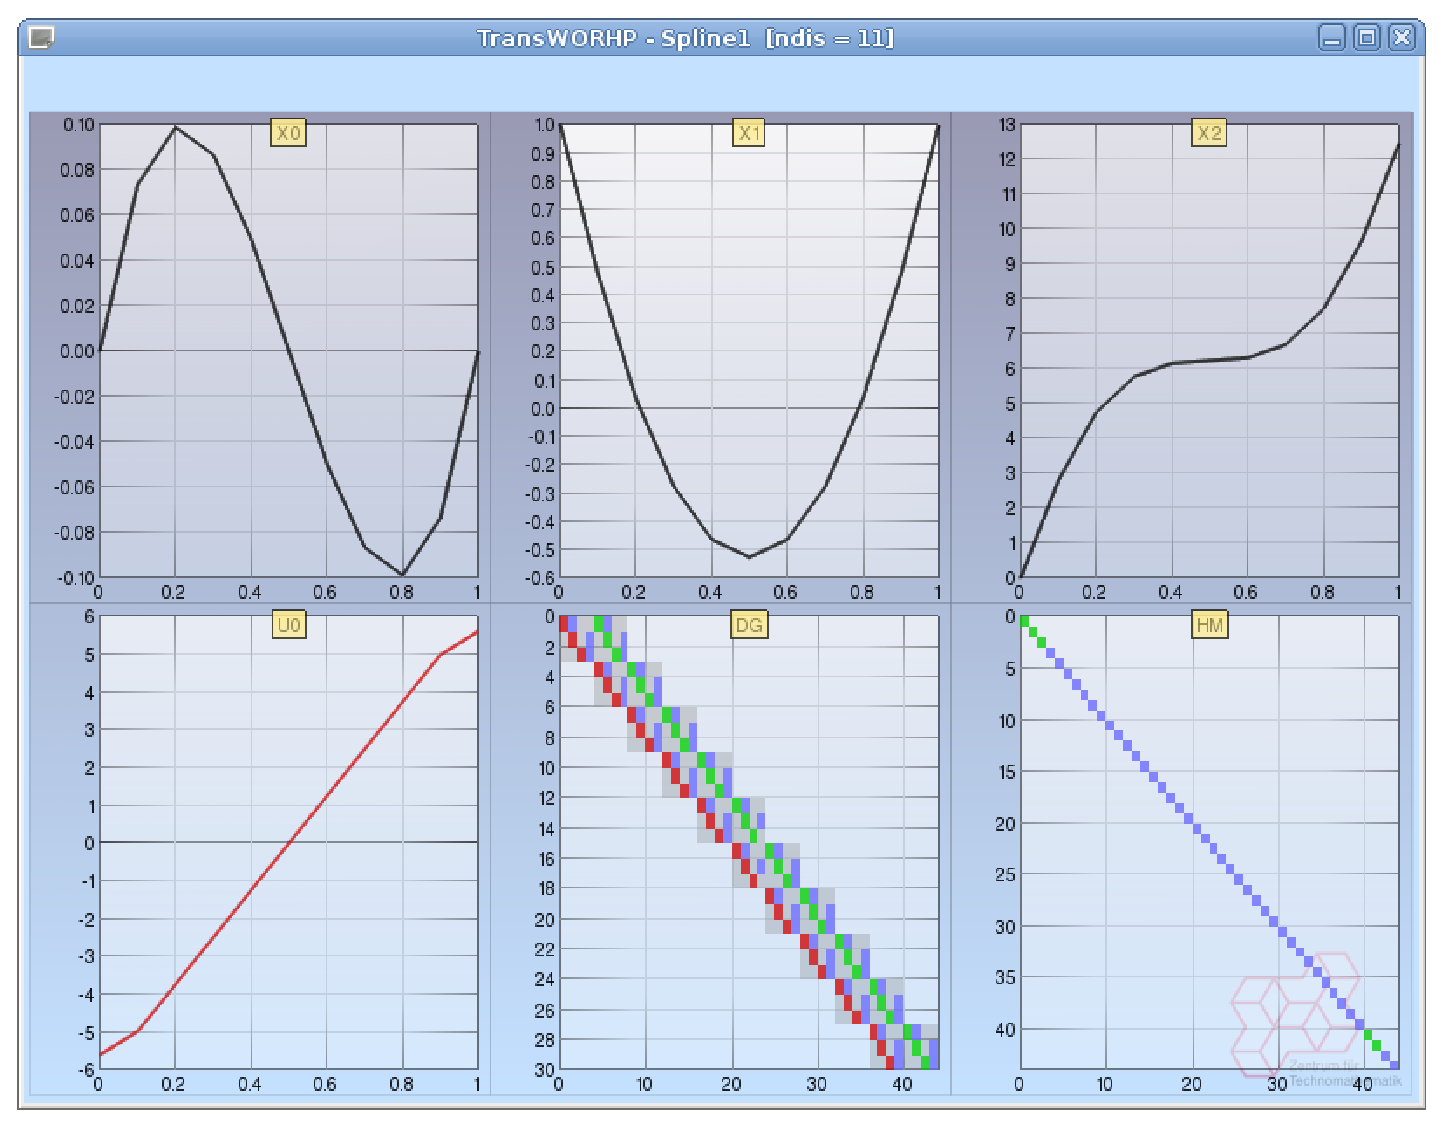
\includegraphics[width=10cm]{images/spline1}
\caption{Grafische Ausgabe}
\label{abb1}
\end{center}
\end{figure}

Zus�tzlich werden die f�r die Optimierung mit WORHP ben�tigte Jacobi-Matrix {\tt DG} und Hesse-Matrix {\tt HM} angezeigt (sparsity). Die Bedeutung der verwendeten Farben zeigt Tab.~\ref{tabfarbe}.


\begin{table}[b]
\begin{center}
\begin{tabular}{r|l}
blau & zuf�lliger Wert\\
rot & $-1$\\
rosa & $-\frac{1}{2}$ \\
gr�n & $1$ \\
grau & Null 
\end{tabular}
\caption{Bedeutung der Farben der angezeigten Matrizen}
\label{tabfarbe}
\end{center}
\end{table}

Nicht eingef�rbte Eintr�ge werden in der Matrix nicht angelegt, und sparen so Speicherplatz und Rechenzeit.

Die Bl�cke der Jacobi-Matrix entstehen dadurch, dass Zust�nde zu diskreten Zeitpunkten nur von benachbarten Zust�nden abh�ngen.

\explain{Abspeichern der Abbildungen als eps mit F1.}

\section{Ableitungsstrukturen in \TransWORHP}

\subsection{Angabe von Ableitungs-Strukturen}
\label{abl1}
Die Rechenzeit kann verringert werden, wenn die Struktur der Jacobi-Matrix besser bekannt ist. In diesem Beispiel l�sst sich die Struktur der Ableitung der rechten Seite leicht angeben.

Die rechte Seite lautete:

$$
\begin{array}{rcl}
	     dx_0 &=& x_1  \\
             dx_1 &=& u_0   \\
             dx_2 &=& u_0^2   \\
\end{array}
$$

Damit h�ngt $dx_0$ nur von $x_1$ ab, $dx_1$ und $dx_2$ nur von $u_0$. 

Diese Struktur wird durch �berladen dieser Methode angegeben:

\syntax{bool ode\_structure(DiffStructure \&s);}

In {\tt DiffStructure} wird angegeben, welche Gleichung von welchen Zust�nden, Steuerungen und Parametern abh�ngt. Dazu dient der Klammer-Operator

\syntax{double\& DiffStructure::operator()(int eq, int var);}
\sparams{
{\tt eq} & Index der zu definierenden Gleichung \\
{\tt var} & Index der Optimierungsgr��e. Dieser wird mit {\tt x\_indexode}, {\tt u\_indexode} oder {\tt p\_indexode} bestimmt. \\
}

\syntax{int p\_indexode(int param);}
\sparams{
{\tt param}   & Koordinate des Parametervektors \\
}

Der R�ckgabewert von {\tt ode\_structure} bestimmt, ob die Struktur auch verwendet wird.

{\footnotesize
\ccccode{spline2.cpp}{Ableitungsstrukturen der rechten Seite: spline2.cpp}{35}{41}
}

Die entstehende Jacobi-Matrix ist in Abb. \ref{fig2} dargestellt.

\begin{figure}
\begin{center}
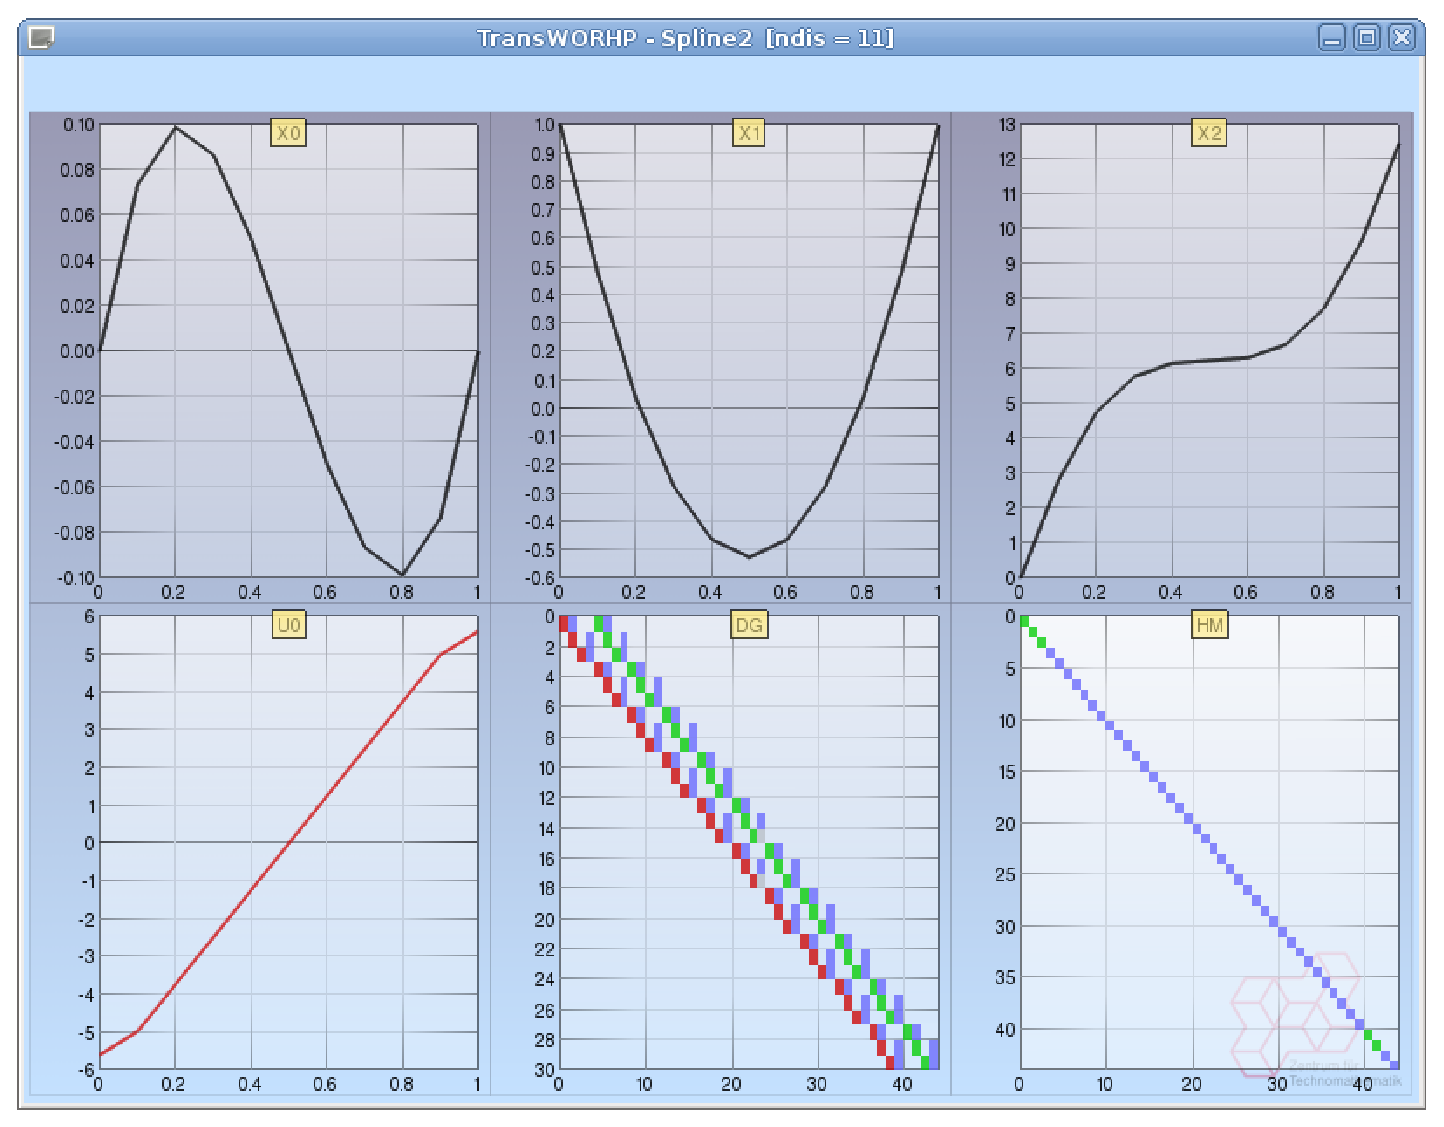
\includegraphics[width=10cm]{images/spline2}
\caption{Jacobi-Matrix mit optimaler Ausnutzung der Sparsity}
\label{fig2}
\end{center}
\end{figure}



Analog wird in diesem Beispiel auch die Struktur der Ableitung der Zielfunktion angegeben. Hier ist diese Methode zu �berladen:

\syntax{bool obj\_structure(DiffStructure \&s);}

Da die Zielfunktion nur aus einer Gleichung besteht, ist hier der Parameter {\tt eq} auf 0 zu setzen.



{\footnotesize
\ccccode{spline2.cpp}{Ableitungsstrukturen der Zielfunktion: spline2.cpp}{21}{25}
}



\subsection{Angabe der ersten Ableitungen}

Um numerische Ableitungen mit finiten Differenzen zu umgehen -- diese werden bei sehr vielen  diskreten Punkten ungenauer als der Diskretisierungsabstand -- bietet sich die analytische Angabe von Ableitungen an.

Die rechte Seite lautete:
$$
\begin{array}{rcl}
	     dx_0 &=& x_1  \\
             dx_1 &=& u_0   \\
             dx_2 &=& u_0^2   \\
\end{array}
$$

Die nicht verschwindenden analytischen Ableitungen sind

$$
\begin{array}{rcl}
	    \displaystyle \frac{\partial dx_0}{\partial x_1} &=& 1  \\
            \displaystyle \frac{\partial dx_1}{\partial u_0} &=& 1   \\
             \displaystyle\frac{\partial dx_2}{\partial u_0} &=& 2 u_0   \\
\end{array}
$$

Um diese in \TransWORHP\ anzugeben, wird wieder eine Methode �berladen:

\syntax{bool ode\_diff(DiffStructure \&s, double t, const double *x, const double *u, const double *p);}

{\tt t}, {\tt x}, {\tt u} und {\tt p} entspricht der Bedeutung aus der Funktion {\tt ode}. 

Der Klammer-Operator aus Abschnitt \ref{abl1} gibt eine Referenz auf einen Speicherplatz zur�ck, der mit den berechneten Ableitungen beschrieben wird.

{\footnotesize
\ccccode{spline3.cpp}{Analytische Ableitungen der rechten Seite: spline3.cpp}{49}{56}
}

Analog f�r die Zielfunktion:

\syntax{bool obj\_diff(DiffStructure \&s);}


{\footnotesize
\ccccode{spline3.cpp}{Analytische Ableitungen der Zielfunktion: spline3.cpp}{27}{31}
}


\section{Allgemeine Optimalsteuerprobleme mit \TransWORHP}
\subsection{Angabe von Startsch�tzungen}

Bei komplexeren Optimierungsproblemen ist die Angabe von sinnvollen Startsch�tzungen wichtig, um Konvergenz zu sichern oder die Konvergenzgeschwindigkeit zu verbessern.


Hierf�r werden wieder Methoden �berladen:

\syntax{
void x\_init(double *x, int i, int dis)

void u\_init(double *u, int i, int dis)

void p\_init(double *p)}

{\tt x\_init} und {\tt p\_init} werden f�r jeden diskreten Punkt aufgerufen. Der aktuelle Index {\tt i} sowie die Gesamtzahl der Punkte {\tt dis} stehen bereit.

Anmerkung: Je nach gew�hlter Diskretisierungsmethode (Trapez, Hermite-Simpson) kann {\tt dis} variieren.

{\footnotesize
\ccccode{spline4.cpp}{Startsch�tzung der Steuerung: spline4.cpp}{80}{83}
}

\subsection{Randwerte}

Einfache Anfangs- und Endwerte, bzw. beliebige Werte dazwischen k�nnen mit {\tt var\_boundary} angegeben werden.

Um komplexere Randbedingungen f�r einzelne Zeitpunkte zu formulieren, k�nnen Gleichungen der Form $$r(x,u)=0$$ hinzugef�gt werden. Die Anzahl der Gleichungen ist im Konstruktor von \TransWORHP\ anzugeben.

Die Randbedingungen k�nnen mit {\tt x()}, {\tt u()}, {\tt p()} wie in Abschnitt \ref{zf} formuliert werden.

\syntax{void rand(double *r);}

Analog lassen sich auch wieder die Ableitung der Randwerte sowie deren Struktur angeben:

\syntax{bool rand\_structure(DiffStructure \&s);}

\syntax{bool rand\_diff(DiffStructure \&s)}

Es k�nnen Ober- und Untergrenzen angegeben werden f�r Bedingungen der Form:
$$ r_{low} \le r(x,u) \le r_{upp}$$

\syntax{void rand\_boundary(double *r\_low, double *r\_upp);}
	

Auf diese Weise lassen sich auch (weniger effizient) die gegebenen Anfangs- und Endbedingungen festlegen:
{\footnotesize
\ccccode{spline5.cpp}{Randwerte: spline5.cpp}{82}{127}
}

%Achtung: Derzeit muss bei Verwendung von rand auch die Struktur angegeben werden!

\subsection{Nebenbedingungen}

\explain{Einfache Steuer- und Zustandsbeschr�nkungen (Box-Beschr�nkungen) k�nnen mit 
{\tt x\_boundary}, {\tt u\_boundary} und {\tt p\_boundary} formuliert werden. Diese Funktionen sollte man auch benutzen, da sie effektiver sind.}

Die Anzahl der Nebenbedingungen ({\tt n\_neben}) muss im Konstruktor von \TransWORHP\ angegeben werden. F�r komplexere Beschr�nkungen wird diese Methode �berladen:
	
\syntax{void neben(double *c, double t, const double *x, 
			   const double *u, const double *p)}


{\tt t}, {\tt x}, {\tt u} und {\tt p} entsprechen dem Aufruf von {\tt ode()} in Abschnitt \ref{zf}.

Es m�ssen Ober- und Untergrenzen angegeben werden:

\syntax{void neben\_boundary(double *c\_low, double *c\_upp);}

	
Die Struktur und die Werte der Ableitungen der Nebenbedingungs-Gleichungen kann zus�tzlich angegeben werden:

\syntax{bool neben\_structure(DiffStructure \&s);

bool neben\_diff(DiffStructure \&s, double t, const double *x, 
                 const double *u, const double *p);}



Im Beispiel wird zus�tzlich 
$$-0.4 \le x_0 + x_1 \le 1 $$
gefordert. Diese Gleichung h�ngt von $x_0$ und $x_1$ ab, was in der Struktur vorgegeben wird.
	
{\footnotesize
\ccccode{spline5.cpp}{Nebenbedingungen: spline5.cpp}{130}{155}
}


\section{N�chste Schritte}

Optionale Erweiterungen zur L�sung von Optimalsteuerungsproblemen werden hier vorgestellt. Grundlage ist jeweils das Spline-Problem in der Version spline4.cpp.


\subsection{Startsch�tzung durch Integration}

Sind die ungef�hre Struktur der Steuerung und die Anfangswerte der Zust�nde bekannt, kann dieses als Startsch�tzung angegeben und damit die Zust�nde f�r alle Zeitpunkte hochintegriert werden. Dadurch entsteht eine Startsch�tzung f�r die Zust�nde. Hierzu wird die Funktion

\syntax{int Integrate(int btableau);}

genutzt, welcher durch den L�ser ({\tt solver}) bereitgestellt wird.

{\footnotesize
\ccccode{spline_ruku.cpp}{Startsch�tzung durch Integration: spline\_ruku.cpp}{105}{118}
}

\subsection{Ergebnisse zwischenspeichern}

Genauere L�sungen lassen sich durch eine h�here Anzahl an Diskretisierungspunkten erreichen. Da eine L�sung auf einem sehr feinen Gitter viel Rechenzeit in Anspruch nimmt, ist eine gute Startsch�tzung n�tig. Diese l�sst sich beispielsweise durch eine L�sung auf einem gr�beren Gitter erzeugen. Zum Speichern einer L�sung wird die Funktion {\tt ToMatlab()} benutzt. Anschlie�en kann vor der erneuten Optimierung (vor {\tt Loop()}) die zuvor erstellte L�sung mit {\tt FromMATLAB()} eingelesen werden. Beide Methoden werden vom {\tt solver} bereitgestellt. Hierbei werden Zwischenpunkte interpoliert.

\syntax{void ToMATLAB(const std::string\& filename);\\
void FromMATLAB(const std::string\& filename);}

{\footnotesize
\ccccode{spline_load.cpp}{schreiben und laden einer Startsch�tzung: spline\_load.cpp}{88}{126}
}

\subsection{Automatische Differentiation}

Experimentell. Bereitstellen der Funktionen obj und ode f�r MagicDoubles. 

Beispiel:

TODO spline\_ad.cpp

Details sp�ter in Abschnitt \ref{magicdbl}.


\subsection{Lagrange-Term im Zielfunktional}

Experimentell. Angabe von Integrandenfunktionen (mit Ableitungen) und Gewichtung, die zum Mayer-Zielfunktional obj() hinzuaddiert wird.

Vgl. \ref{intlag1}

TODO spline\_int.cpp


\subsection{Explizite Integrationsverfahren}

TODO spline\_expl.cpp


\subsection{Sensitivit�tsanalyse mit WORHP Zen}

TODO spline\_zen.cpp

\subsection{Adaptive Gitteranpassung}

F�r die adaptive Gitteranpassung muss lediglich {\tt Loop()} durch {\tt meshRef()} ersetzt werden. Einstellungen k�nnen in der XML-Datei vorgenommen werden (vgl. \ref{meshRef}).

\syntax{int meshRef();}

\explain{Es ist darauf zu achte, dass w�hrend die Gitteranpassung mit grafischer Ausgabe (also mit aktiviertem {\tt viewer}) l�uft, das Fenster nicht via Klick auf Schlie�en geschlossen wird. Dies k�nnte Speicherfehler hervorbringen! Nach jedem Anpassungsschritt schlie�t und �ffnet sich das Fenster selbstst�ndig.}

{\footnotesize
\ccccode{../example/rakete_meshRef.cpp}{adaptive Gitteranpassung: rakete\_meshRef.cpp}{95}{123}
}

\subsection{Mehrere Phasen}

Es ist m�glich mehrere Optimalsteuerprobleme (Phasen) in einem TWfolder zu vereinen. Dies ist exemplarisch in spline\_phase.cpp dargestellt. Hier wurde das Splineproblem in zwei Phasen aufgeteilt. So wurden in der ersten Phase die Anfangswerte angegeben, aber die Endwerte frei gelassen. In der zweiten Phasen entsprechend andersherum. Dies l�sst sich mit Fallunterscheidungen in {\tt var\_boundary()} realisieren.

{\footnotesize
\ccccode{spline_phase.cpp}{mehrere Phasen: spline\_phase.cpp}{69}{80}
}

Damit Stetigkeit zwischen beiden Phasen herrscht, m�ssen weitere Nebenbedingungen angegeben werden. Hierzu muss zun�chst von {\tt TWfolder} geerbt und die Anzahl der Nebenbedingungen angegeben werden. Hierzu stehen folgende Methoden zur Verf�gung:

\syntax{void g\_boundary(double *x\_low, double *x\_upp);\\
void con(double *C);\\
bool con\_structure(DiffStructure \&s);\\
bool con\_diff(DiffStructure \&s, int colindex);}

Diese Methoden verhalten sich analog zu den bereits beschriebene (vgl. z.B. {\tt neben()}). Allerdings ist es (bis jetzt) nur m�glich lineare Nebenbedingungen anzugeben. Zugriff auf die Phasen besteht �ber den Vektor {\tt phases}:

\syntax{std::vector<TransWorhp*> phases;}

Zu beachten ist, dass beim Zugriff auf Zust�nde oder Steuerungen aus einzelnen Phasen ein Offset ({\tt Delta1}) addiert werden muss. Weiterhin muss beachtet werden, dass der Zugriff direkt auf dem WORHP Optimierungsvektor erfolgt.

{\footnotesize
\ccccode{spline_phase.cpp}{mehrere Phasen: spline\_phase.cpp}{105}{114}
}

\subsubsection*{Internes zusammensetzen mehrere Phasen}

Werden mehrere Phasen verbunden, so erstellt \TransWORHP\ intern ein einziges (gro�es) Problem daraus. Hierzu werden die einzelnen Phasen nacheinander in den Optimierungsvektor von WORHP geschrieben. Dies ist in Abbildung \ref{abb:splinePhase} anhand der Struktur von {\tt DF} bzw. {\tt DG} gut zu erkennen.

\begin{figure}[h]
\begin{center}
\includegraphics[width=7cm]{images/spline/pix_5_DF_phase}
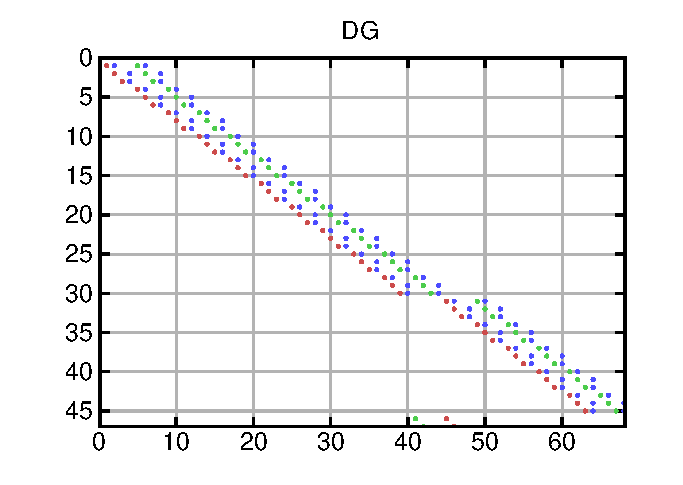
\includegraphics[width=7cm]{images/spline/pix_6_DG_phase}
\caption{Spline-Problem mit zwei Phasen}
\label{abb:splinePhase}
\end{center}
\end{figure}



\chapter{Funktions�bersicht}

In diesem Kapitel werden die wichtigsten Funktionen erkl�rt.

\section{Die Klasse {\tt TransWorhp}}

Von dieser Klasse werden alle Probleme abgeleitet.

\subsection{Systemmethoden}

Konstruktor 

\syntax{TransWorhp(const std::string \&s, int dis, int ode, int ctrl, int param, int rand, int neben);}

Destruktor

\syntax{\textasciitilde TransWorhp();}

WORHP-Arbeitsspeicher anlegen und mit Instanz verkn�pfen:

\syntax{int Init(XMLNode *xml, OptVar \&o, Workspace \&w, Params \&p, Control \&c, Viewer *viewer=0);}

XML-Dateien lesen:

\syntax{static XMLNode *ReadParams(const std::string\& filename);}

Optimierungsschleife:

\syntax{int Loop();}


\subsection{Zugriffsmethoden}

Die Zust�nde und Steuerungen werden in den Optimierungsvektor von WORHP geschrieben. Damit komfortabel auf einzelne von ihnen zugegriffen werden kann, stehen verschiedene Funktionen bereit. Steuerung und der Zustand lassen sich zu jedem diskreten Zeitpunkt {\tt dis} mit folgenden Methoden auslesen. Da freie Parameter f�r alle Zeitpunkte gleich sind, gibt es nur einen Wert.

\syntax{double x(int dis, int ode) const;

	double u(int dis, int ctrl) const;

	double p(int param) const;
}

Wird das Optimalsteuerungsproblem mit Verfahren h�herer Ordnung (z.B Hermite-Simpson) gel�st, werden Zwischenpunkte eingef�gt. An diesen Punkten l�sst sich ebenfalls der Zustand und die Steuerung auslesen. Die Methoden {\tt x\_\_()} und {\tt u\_\_()} laufen �ber alle Punkte, wohingegen die Methoden {\tt x()} und {\tt u()} nur an den 'Haupt'punkten auswerten und alle Zwischenpunkte �berspringen.

\syntax{double x\_\_(int dis, int ode) const;

double u\_\_(int dis, int ctrl) const;
}

Indexbestimmung 

\syntax{
	int x\_index(int dis, int ode);

	int u\_index(int dis, int ctrl);

	int p\_index(int param);

	int p\_indexode(int param);
}
	
\subsection{Implementierung des OCP}

\subsubsection{�berladbare Methoden}


Zielfunktion 

	\syntax{double obj();

bool obj\_structure(DiffStructure \&s);

bool obj\_diff(DiffStructure \&s);
}
	
	
ODE-System

	\syntax{
void ode(double *dx, double t, const double *x, const double *u, const double *p);

	bool ode\_structure(DiffStructure \&s);

	bool ode\_diff(DiffStructure \&s, double t, const double *x, const double *u, const double *p);

	bool ode\_diff\_p(DiffStructure \&s, double t, const double *x, const double *u, const double *p, int index);
	}

(letztere Funktion bestimmt ausschlie�lich die Ableitung nach Parametern!)


Box-Beschr�nkungen

	\syntax{void x\_boundary(double *x\_low, double *x\_upp);

	 void u\_boundary(double *u\_low, double *u\_upp);

	 void p\_boundary(double *p\_low, double *p\_upp);

	 void var\_boundary(double *x\_low, double *x\_upp);
}

Rand-Bedingungen

\syntax{	 void rand(double *r);

	 void rand\_boundary(double *r\_low, double *r\_upp);

	 bool rand\_structure(DiffStructure \&s);

	 bool rand\_diff(DiffStructure \&s);
}

	Nebenbedingungen

	\syntax{void neben(double *c, double t, const double *x, const double *u, const double *p);

	 void neben\_boundary(double *c\_low, double *c\_upp);

	 bool neben\_structure(DiffStructure \&s);

	 bool neben\_diff(DiffStructure \&s, double t, const double *x, const double *u, const double *p);

	 bool neben\_diff\_p(DiffStructure \&s, double t, const double *x, const double *u, const double *p, int index);
	}

	Startsch�tzung

\syntax{ void init();

	 void p\_init(double *p);

	 void x\_init(double *x, int i, int dis);

	 void u\_init(double *u, int i, int dis);
}

\subsection{I/O-Methoden}

\subsubsection{�berladbare Methoden}

Aufruf in jedem Iterationschritt f�r Konsolen- oder Datei-Ausgabe:

\syntax{	
int step();
}
Wird 0 zur�ckgegeben, wird die Optimierung unterbrochen.

Aufruf am Ende der Optimierung f�r Konsolen- oder Datei-Ausgabe:

\syntax{	
void terminate();
}


\subsubsection{Grafisches Interface}

Weitere Plots erzeugen und Plots beschriften:

\syntax{void OpenWindows(Viewer *gr);

std::string GetXTitle(int d);

std::string GetUTitle(int d);
}

\subsection{Weiterf�hrende Methoden}

Zeitdiskretisierung anpassen, z.B. im Konstruktor:	

\syntax{void TimeAxis(double exponent);}
oder manuell.





Zustand oder Steuerung an beliebigem Zeitpunkt auslesen:

\syntax{
	void GetState(double *x, double t);

	void GetControl(double *u, double t);
	}


\section{Die Struktur {\tt DiffStructure}}

Eintr�ge in den Ableitungsmatrizen k�nnen angelegt und gesetzt werden durch den Klammeroperator:

\syntax{
	double\& operator()(int i, int j);
}

\subsection{Zugriff auf DiffStructure}

Mit Hilfsfunktionen wird der richtige Index zugeordnet.

lokale Strukturen (ode, integral, neben):
Zugriff mit x\_indexode

globale Strukturen (rand, obj):
Zugriff mit x\_index

TODO: Bild

\section{Die Klasse {\tt Viewer}}

In {\tt OpenWindows()} k�nnen neue Plots hinzugef�gt werden:

Struktur der Ableitungs-Matrix plotten

\syntax{
	void Matrix(const std::string \&s, WorhpMatrix *m);
}

Daten plotten, die in einer Funktion {\tt func} bereitgestellt werden:

\syntax{
	void Data(const std::string \&s, Funktionenzeiger2 func, int lo, int hi, int index);
}

Dabei ist {\tt func} von diesem Typ:
 
\syntax{
typedef double (*Funktionenzeiger2) (int \&len, int \&ndgl, int \&nsteuer,
                                     double *t,double *x, double *u, int \&i, int \&index);
}
{\tt index} kann zur internen Unterscheidung verwendet werden.

Phasen-Diagramm plotten (also Daten {\tt func(..., d1)} gegen {\tt func(..., d2)}).

\syntax{
	void PhasePlot(const std::string \&s, Funktionenzeiger2 func, int d1, int d2);
}

OpenGL-Plot hinzuf�gen.

\syntax{
	void ThreeD(const std::string \&s, XMLNode *xml, plot3d f);
}

Dabei ist {\tt f} von diesem Typ:

\syntax{
typedef void (*plot3d) (glObject *obj, double *x, double t);
}

\example{Animation von Objekten

Modell mit Cinema4D erstellen und mit riptide exportieren. 
}

Vergleichswerte hinzuf�gen:

\syntax{
	void AddCompareCurve(int \&cmpstep, double* cmp, double* cmptime, int n);
}

Alle Plots schlie�en oder neu anordnen:

\syntax{
	void CloseAll();
	void TilePlots();
}


%	void SetHeader(char *s, int mode);

%	void AutoScale();


%	size_t Size() const;

%	void SetFloatTime(double t);
%	void SetTimeIsTime();

		
\section{Die Klasse {\tt MagicDouble}}
\label{magicdbl}

Automatische Berechnung der 1. und 2. Ableitung.

TODO

\chapter{Grafisches Interface}

Erkl�rung der Menu-Punkte, Maus- und Tastatursteuerung, etc.





\section{�berpr�fen der analytischen Ableitungen}

Angabe von analytische Ableitungen bevorzugt, da stabiler.

Wie lassen die sich auf Korrektheit �berpr�fen?

Man setze in {\tt transworhp.xml}
\begin{verbatim}
        <USERDF>-1</USERDF>
        <USERDG>-1</USERDG>
        <USERHM>-1</USERHM>
\end{verbatim}
um die Ableitungsberechnung von WORHP zu verwenden.

Dann l�sst man das Programm normal laufen, und w�hlt am Ende der Optimierung im erscheinenden Menu am oberen Fensterrand Debug->Check DF bzw. 
Debug->Check DG (oder dr�ckt einfach F9 bzw. F10).

Dann erscheint eine lange Ausgabe bestehend aus Matrix-Index, numerischem Ableitungswert und dem vorgegebenen Ableitungswert.

Wo sich die Werte stark unterscheiden, erscheint ein Pfeil, und der Text ist rot. 

\chapter{Beispiele}

\addtocontents{lof}{\vspace*{.5cm}{\bf 6~~Beispiele\\}}
%\addtocontents{lot}{\vspace*{.5cm}{\bf 6~~Beispiele\\}}


Im Ordner {\tt example} finden sich umfangreichere Beispiele:


%%%%%%%%%%%%%%%%%%%%%%%%%%%%%%%%%%%%%%%%%%%%%%%%%%%%%%%%%%%%%%%%%%%%%%%%%%%%%55

\section{Chemischer Reaktor}

Bei diesem Modell handelt es sich um eine zweistufige Reaktionsgleichung zur Umwandlung einer chemischen Substanz. Der Temperatur im Reaktor kann durch die Steuerung beeinflusst werden, um die Umwandlung zu beg�nstigen. Ziel ist es, die Konzentration der entstehenden Substanz $x_2$ im Endpunkt zu maximieren. 

$$\begin{array}{crclrcll} \displaystyle\min_{x,u} &\multicolumn{3}{l}{-x_2(1)}\\ 
\text{unter} &\dot x_1(t) &=& -u(t)\cdot x_1(t) + u(t)^2\cdot x_2(t) \\
             &\dot x_2(t) &=&  u(t)\cdot x_1(t) -3\cdot u(t)^2\cdot x_2(t) \\[.1cm] 
             &x_1(0) &=& 1 \\ 
             &x_2(0) &=& 0 \\[.1cm] 
             &u(t)&\in&\multicolumn{5}{l}{[0;1],\quad t\in[0;1]}
\end{array}$$

Quelle: 8.16 bzw. Skript?


\begin{figure}[h]
\begin{center}
\begin{tabular}{|c|c|c|}
\hline
Anzahl Punkte & Zielfunktionswert & Rechenzeit\\\hline
21        &  -0.28810463835 & \\\hline
\end{tabular}

\includegraphics[width=5cm]{images/chemie/pix_1_x_1}
\includegraphics[width=5cm]{images/chemie/pix_2_x_2}
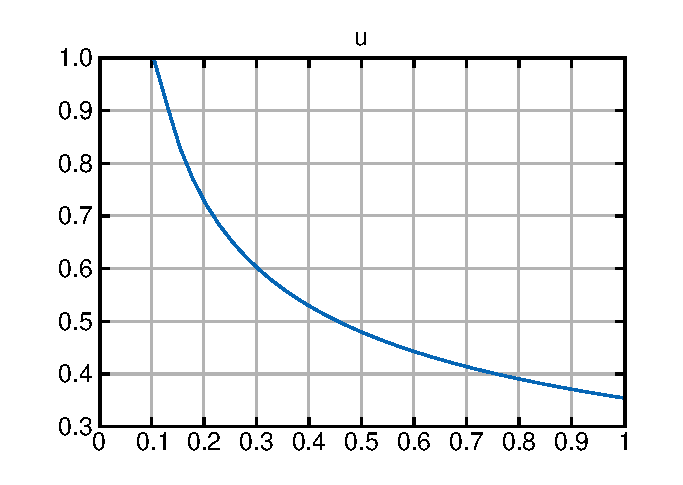
\includegraphics[width=5cm]{images/chemie/pix_3_u}

% \includegraphics[width=5cm]{images/chemie/pix_4_DF}
% 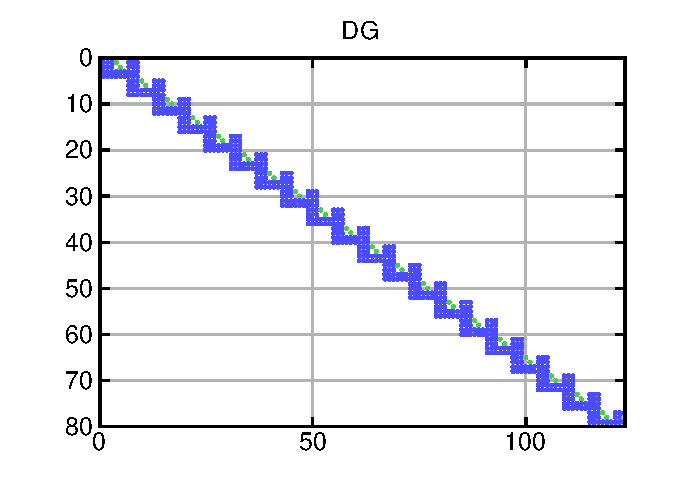
\includegraphics[width=5cm]{images/chemie/pix_5_DG}
% 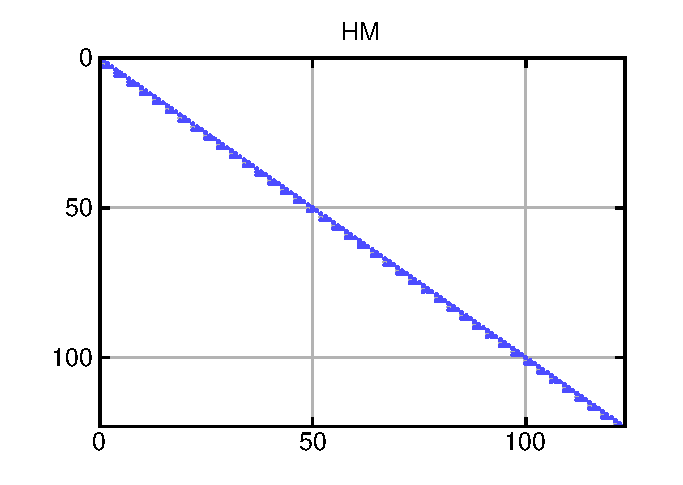
\includegraphics[width=5cm]{images/chemie/pix_6_HM}

\label{ex:chemie}
\caption{Chemischer Reaktor}
\end{center}
\end{figure}


%%%%%%%%%%%%%%%%%%%%%%%%%%%%%%%%%%%%%%%%%%%%%%%%%%%%%%%%%%%%%%%%%%%%%%%%%%%%%55
\newpage
\section{Spline}

Interpolation durch kubischen Spline als Optimierungsaufgabe.

$$\begin{array}{crclrcll} \displaystyle\min_{x,u} &\multicolumn{3}{l}{\frac{1}{2} x_3(1)}\\ 
\text{unter} &\dot x_1(t) &=& x_2(t) \\
             &\dot x_2(t) &=&  u(t) \\
	     &\dot x_3(t) &=&  u^2(t) \\[.1cm]  
             &x_1(0) &=& 0 &  &x_1(1) &=& 0 \\
             &x_2(0) &=& 1  & &x_2(1) &=& -1\\
	     &x_3(0) &=& 0 \\[.1cm] 
             &x_1(t)&\le&\multicolumn{5}{l}{\alpha,\quad t\in[0;1]}
\end{array}$$

$\alpha > 1/4$: unbeschr�nkt

$1/6<\alpha<1/4$: Ber�hrpunkt

$1/6>\alpha$: Randst�ck



\begin{tabular}{ll}
Diskretisierung & 21 Punkte\\
Zielfunktionswert $\alpha=0$ & 1.9999986332\\
Zielfunktionswert $\alpha=\frac{1}{6}$ &  2.6666658193
\end{tabular}

Quelle: 10.14 bzw. Skript?



\begin{figure}[h]
\begin{center}
\includegraphics[width=5cm]{images/spline/pix_1_x_1}
\includegraphics[width=5cm]{images/spline/pix_2_x_2}
\includegraphics[width=5cm]{images/spline/pix_3_x_3}
\includegraphics[width=5cm]{images/spline/pix_4_u}

% 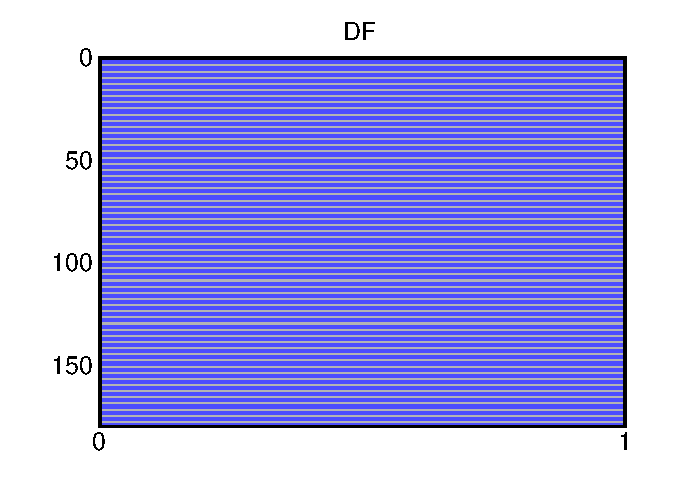
\includegraphics[width=5cm]{images/spline/pix_5_DF}
% 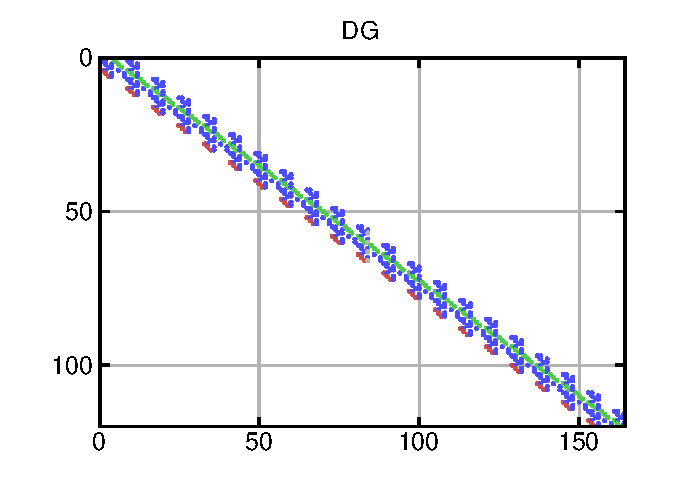
\includegraphics[width=5cm]{images/spline/pix_6_DG}
% 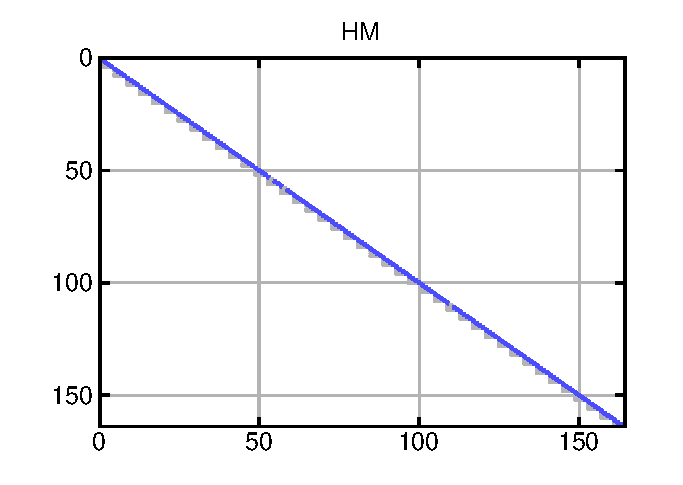
\includegraphics[width=5cm]{images/spline/pix_7_HM}

\label{ex:spline}
\caption{L�sung Spline-Problem mit $\alpha=\frac{1}{6}$}
\end{center}
\end{figure}


\explain{Das Programm zeigt, wie sich Parameter �ber die Kommandozeile variieren lassen.
Hierzu wird eine map der Kommandozeilenparameter ausgelesen.

Die Beschr�nkung $\alpha$ l�sst sich �ber --c steuern.
}

\verb+spline -n 21 --c 0.166666+









%%%%%%%%%%%%%%%%%%%%%%%%%%%%%%%%%%%%%%%%%%%%%%%%%%%%%%%%%%%%%%%%%%%%%%%%%%%%%55
\newpage
\section{Unged�mpfter harmonischer Oszillator}
Beispiel mit freier Endzeit. Die freie Endzeit wird in $p_0$ abgelegt. Das DGl-System muss mit $p_0$ multipliziert werden.


$$\begin{array}{crclrcll} \displaystyle\min_{x,u,t_f} &\multicolumn{3}{l}{t_f}\\ 
\text{unter} &\dot x_1(t) &=& x_2(t) \\
             &\dot x_2(t) &=& -x_1(t)+u(t) \\[.1cm]    
             &x(0)        &=& \left(\begin{array}{c}3\\1\end{array}\right) 
             &x(t_f)      &=& \left(\begin{array}{c}0\\0\end{array}\right) \\[.1cm] 
             &u(t)&\in&[-1;1],& t\in[0;t_f]
\end{array}$$


\begin{tabular}{ll}
Diskretisierung & 51 Punkte\\
Zielfunktionswert & 5.2160656622\\
\end{tabular}

Quelle: 5.19


\begin{figure}[h]
\begin{center}
\includegraphics[width=5cm]{images/oszillator/pix_1_x_1}
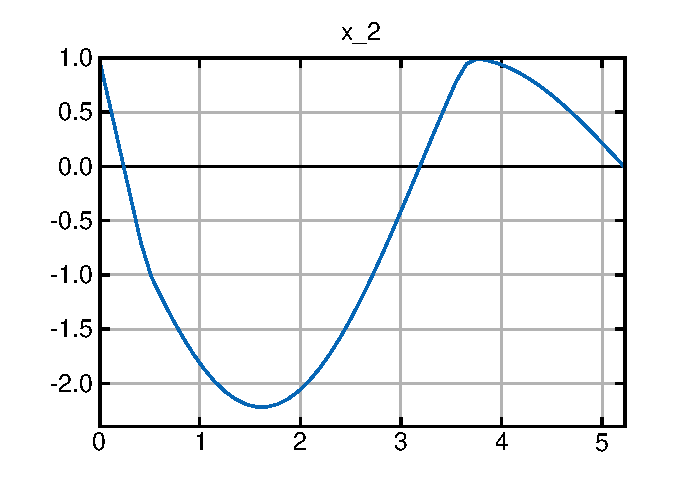
\includegraphics[width=5cm]{images/oszillator/pix_2_x_2}
\includegraphics[width=5cm]{images/oszillator/pix_3_u}

\label{ex:oszillator}
\caption{L�sung Oszillator-Problem}
\end{center}
\end{figure}

\explain{
{\tt freetime = 1;} stellt freie Endzeit auch im Viewer dar.
}




\newpage
\section{Raketenwagen}

Gasgeben und Bremsen.



$$\begin{array}{crclrcll} \displaystyle\min_{x,u,t_f} &\multicolumn{3}{l}{t_f}\\ 
\text{unter} &\dot x_1(t) &=& x_2(t) \\
             &\dot x_2(t) &=& u(t) \\[.1cm]    
             &x(0)        &=& \left(\begin{array}{c}4\\-1\end{array}\right) 
             &x(t_f)      &=& \left(\begin{array}{c}0\\0\end{array}\right) \\[.1cm] 
             &u(t)&\in&[-1;1],& t\in[0;t_f]
\end{array}$$


\begin{tabular}{ll}
%Diskretisierung & 51 Punkte\\
%Zielfunktionswert & 5.2160656622\\
\end{tabular}

Quelle: ?


\begin{figure}[h]
\begin{center}
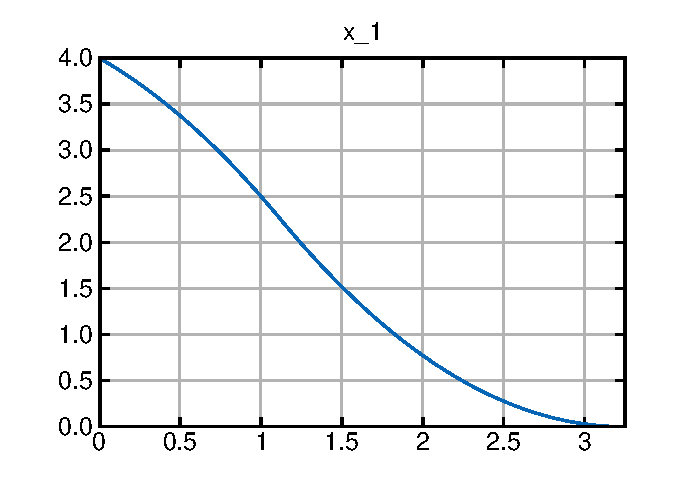
\includegraphics[width=5cm]{images/rakete/pix_1_x_1}
\includegraphics[width=5cm]{images/rakete/pix_2_x_2}
\includegraphics[width=5cm]{images/rakete/pix_3_u}

\label{ex:rakete}
\caption{L�sung Raketenwagen-Problem}
\end{center}
\end{figure}







%%%%%%%%%%%%%%%%%%%%%%%%%%%%%%%%%%%%%%%%%%%%%%%%%%%%%%%%%%%%%%%%%%%%%%%%%%%%%55
\newpage
\section{Erzentlader}

$$\begin{array}{crclrcll} \displaystyle\min_{x,u,t_f} &\multicolumn{3}{l}{t_f}\\ 
\text{unter} &\dot x_1(t) &=& x_2(t) \\
             &\dot x_2(t) &=&  u(t) \\
	     &\dot x_3(t) &=&  x_4(t) \\
	      &\dot x_4(t) &=&  -x_3(t)+u(t) \\[.1cm]    
       &x(0) &=& \left(\begin{array}{c}0\\0\\0\\0\end{array}\right) 
&x(t_f) &=& \left(\begin{array}{c}1\\0\\0\\0\end{array}\right) \\[.1cm] 
             &u(t)&\in&[-1;1],& t\in[0;t_f]\\
	    &x_2(t)&\le&0.2,& t\in[0;t_f]
\end{array}$$





\begin{tabular}{ll}
Diskretisierung & 101 Punkte\\
Zielfunktionswert & 5.84412332892\\
\end{tabular}

Quelle: 10.11


\begin{figure}[h]
\begin{center}
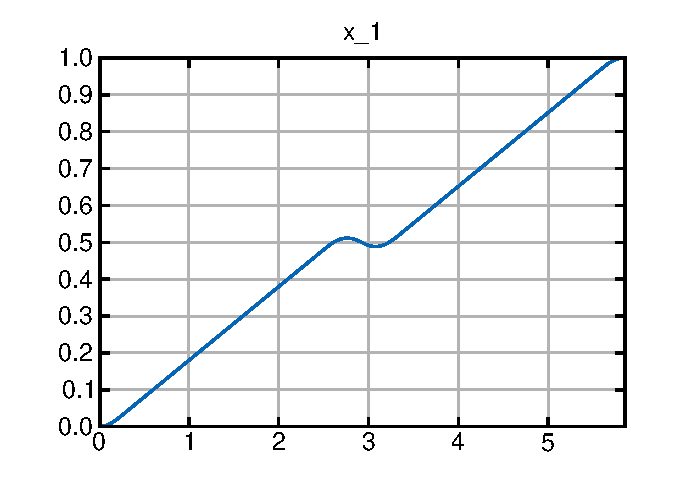
\includegraphics[width=5cm]{images/erzentlader/pix_1_x_1}
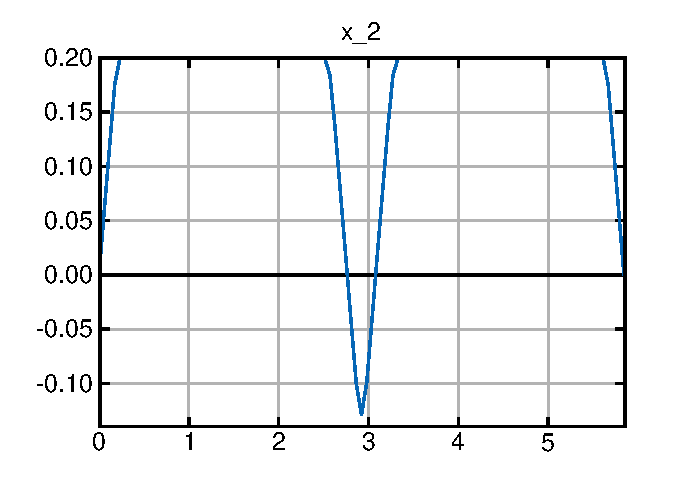
\includegraphics[width=5cm]{images/erzentlader/pix_2_x_2}
\includegraphics[width=5cm]{images/erzentlader/pix_3_x_3}
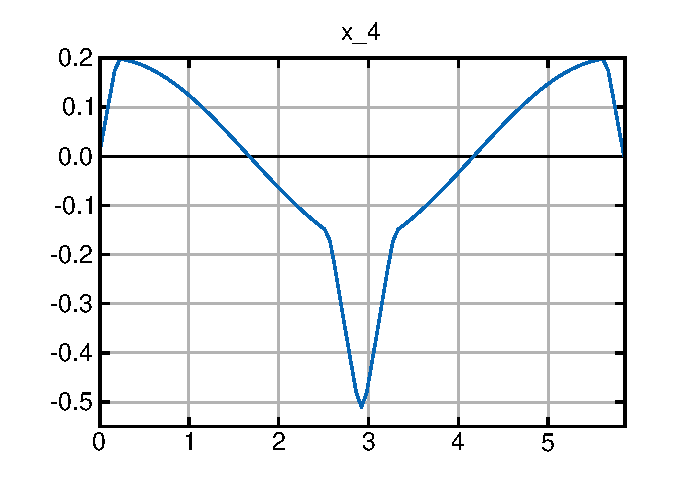
\includegraphics[width=5cm]{images/erzentlader/pix_4_x_4}
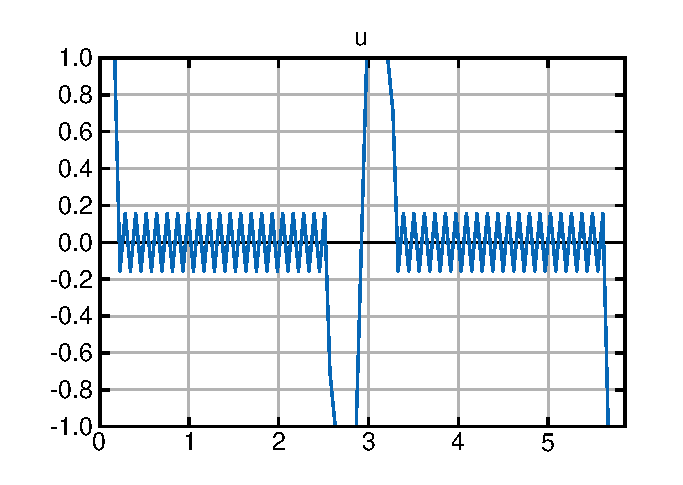
\includegraphics[width=5cm]{images/erzentlader/pix_5_u}


\label{ex:erzentlader}
\caption{L�sung Erzentlader}
\end{center}
\end{figure}






%%%%%%%%%%%%%%%%%%%%%%%%%%%%%%%%%%%%%%%%%%%%%%%%%%%%%%%%%%%%%%%%%%%%%%%%%%%%%55
\newpage
\section{Knickstab}

$$\begin{array}{crclrcll} \displaystyle\min_{x,u} &\multicolumn{3}{l}{\displaystyle\int\limits_0^1 \frac{1}{2} u(t)^2 + \alpha\cdot \cos\theta(t) \, dt}\\ 
\text{unter} &\dot x(t) &=& \sin\theta(t) \\
             &\dot \theta(t) &=&  u(t) \\[.1cm]    
       &x(0) &=& 0   & x(1) &=& 0 \\[.1cm] 
             &x(t)&\in&[-0.05;0.05],& t\in[0;1]
\end{array}$$


\explain{
Alternative Formulierungen als {\tt knickstab.cpp} und {\tt knickstab\_int.cpp}
 mit Lagrange-Term
}

\explain{
TolOpti wird intern h�her gesetzt.
}

\begin{tabular}{ll}
Diskretisierung $\alpha=9.90027$ & 60 Punkte\\
Zielfunktionswert & 9.9002014316\\
\end{tabular}

\begin{tabular}{ll}
Diskretisierung $\alpha=27.2627$ & 51 Punkte\\
Zielfunktionswert & 27.151069208\\
\end{tabular}

\begin{tabular}{ll}
Diskretisierung $\alpha=150$ & 180 Punkte\\
Zielfunktionswert & 148.51217659
\end{tabular}

Quelle: ?




\begin{figure}[h]
\begin{center}
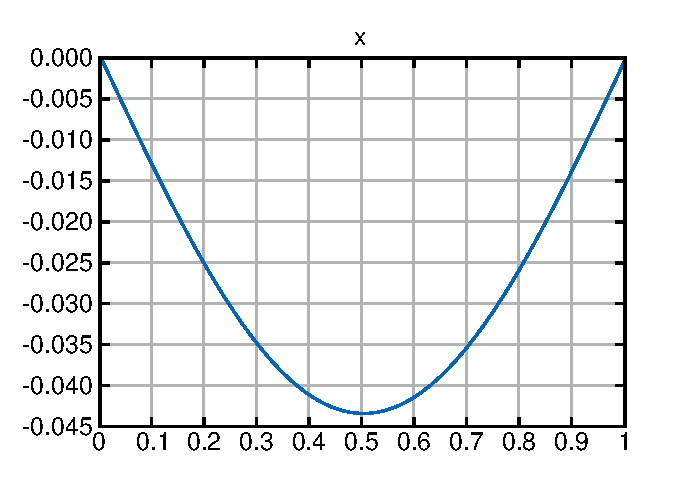
\includegraphics[width=5cm]{images/knickstab_int_9/pix_1_x}
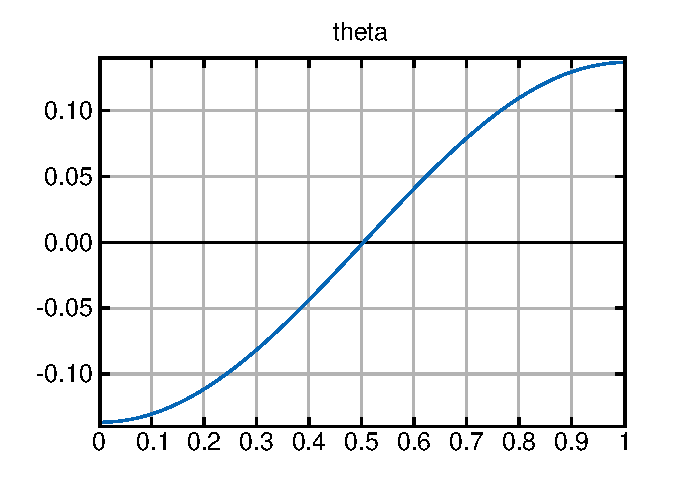
\includegraphics[width=5cm]{images/knickstab_int_9/pix_2_theta}
\includegraphics[width=5cm]{images/knickstab_int_9/pix_3_u}
%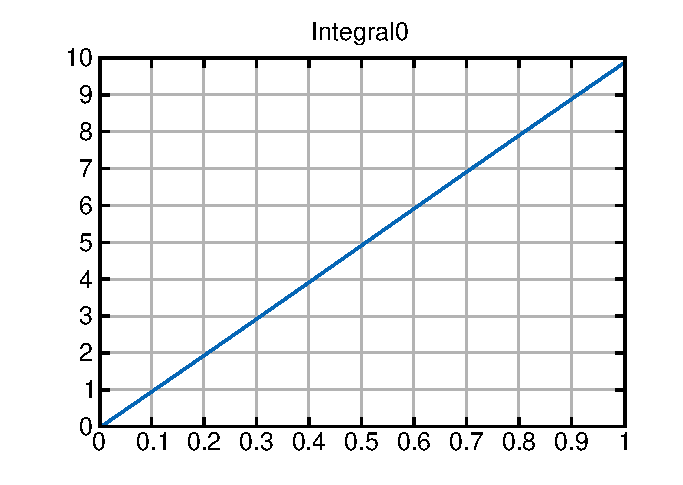
\includegraphics[width=5cm]{images/knickstab_int_9/pix_4_Integral0}

\label{ex:knick1}
\caption{L�sung Knickstab f�r $\alpha=9.90027$}
\end{center}
\end{figure}



\begin{figure}[h]
\begin{center}
\includegraphics[width=5cm]{images/knickstab_int_27/pix_1_x}
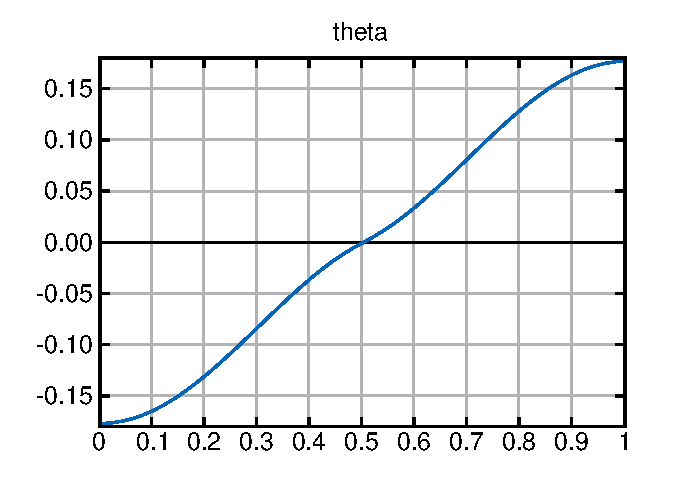
\includegraphics[width=5cm]{images/knickstab_int_27/pix_2_theta}
\includegraphics[width=5cm]{images/knickstab_int_27/pix_3_u}
%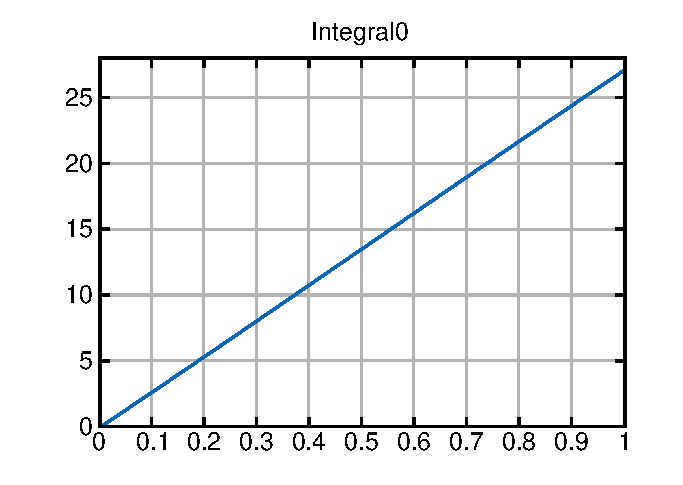
\includegraphics[width=5cm]{images/knickstab_int_27/pix_4_Integral0}

\label{ex:knick2}
\caption{L�sung Knickstab f�r $\alpha=27.2627$}
\end{center}
\end{figure}


\begin{figure}[h]
\begin{center}
\includegraphics[width=5cm]{images/knickstab_int_150/pix_1_x}
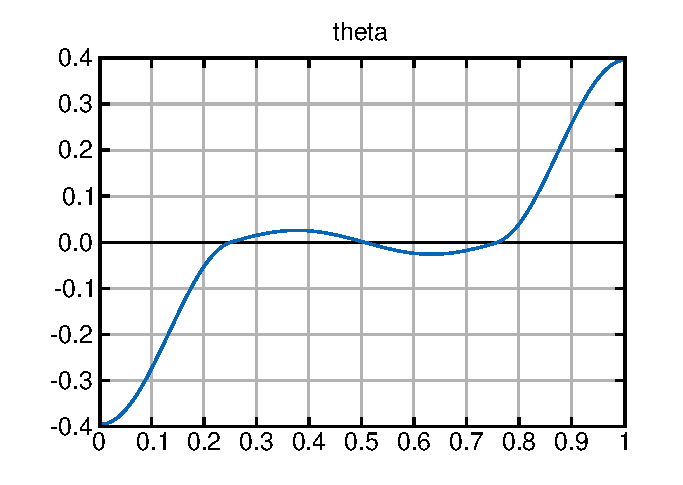
\includegraphics[width=5cm]{images/knickstab_int_150/pix_2_theta}
\includegraphics[width=5cm]{images/knickstab_int_150/pix_3_u}
%\includegraphics[width=5cm]{images/knickstab_int_150/pix_4_Integral0}

\label{ex:knick3}
\caption{L�sung Knickstab f�r $\alpha=150$}
\end{center}
\end{figure}






%%%%%%%%%%%%%%%%%%%%%%%%%%%%%%%%%%%%%%%%%%%%%%%%%%%%%%%%%%%%%%%%%%%%%%%%%%%%%55
\newpage
\section{Reentry-Problem}

$$\begin{array}{crclrcll} \displaystyle\min_{} &\multicolumn{3}{l}{\displaystyle\int\limits_0^{t_f} 10 v^3\sqrt{p_0 e^{-\beta R xi}}}\\ 
\text{unter} &\dot v &=& -\frac{S p v^2}{2m} C_W(u) - \frac{g \sin\gamma}{(1+\xi)^2} \\
  &\dot \gamma &=& -\frac{S p v}{2m} C_A(u) + \frac{v \cos\gamma}{R (1+\xi)} 
- \frac{g \sin\gamma}{v\cdot(1+\xi)^2}\\
             &\dot \xi(t) &=&  \frac{v \sin\gamma}{R} 	      \\[.1cm]    
   \text{mit}  &p &=& p_0 e^{-\beta R\xi}\\
&C_W(u) &=& 1.174 - 0.9\cos u \\
&C_A(u) &=& 0.6\sin u \\[.1cm]
&v(0) &=& 0.36 & v(t_f) &=& 0.27 \\
&\gamma(0) &=& -8.1 \cdot \frac{\pi}{180} & \gamma(t_f) &=& 0 \\
&\xi(0) &=& \frac{4}{R} & \xi(t_f) &=& \frac{2.5}{R}             
\end{array}$$

$$R = 209, \beta = 4.26, p_0 = 2.704\cdot 10^{-3}, g = 3.2172\cdot 10^{-4}, \frac{S}{m} = 53200 $$




\begin{tabular}{ll}
Diskretisierung & 71 Punkte\\
Zielfunktionswert & 0.027911689692\\
Final Time & 225.427        
\end{tabular}

Quelle: ?


\begin{figure}[h]
\begin{center}
\includegraphics[width=5cm]{images/reentry/pix_1_v}
\includegraphics[width=5cm]{images/reentry/pix_2_gamma}
\includegraphics[width=5cm]{images/reentry/pix_3_xi}
\includegraphics[width=5cm]{images/reentry/pix_4_integral}
\includegraphics[width=5cm]{images/reentry/pix_5_u}


\label{ex:reentry}
\caption{L�sung Reentry-Problem}
\end{center}
\end{figure}

\explain{Funktion terminate zur Ausgabe der Verfahrzeit nach Optimierung}

\explain{Funktion step zur Manipulation der L�sung (hier abschneiden auf $[-\pi,\pi]$)}

\explain{alternative formulierung mit sin/cos und Nebenbedingung}



%%%%%%%%%%%%%%%%%%%%%%%%%%%%%%%%%%%%%%%%%%%%%%%%%%%%%%%%%%%%%%%%%%%%%%%%%%%%%55

\newpage
\section{Laufkatze}

Kransystem

\begin{figure}
\begin{center}
\includegraphics[width=10cm]{images/laufkatze}
\caption{3d-Plot der Laufkatze}
\label{abb3}
\end{center}
\end{figure}

\begin{itemize}
\item Standardproblem
\item mit Automatischer Differentiation
\item in Lagrange-Formulierung
\end{itemize}

\begin{align*} \label{eq:laufkateze}
\begin{split}
	\min_{x,u,t_f} \qquad & x_8(t_f) + 0.1 \cdot t_f\\
	\text{unter} \quad \dot{x}_0 &= x_1 \cdot t_f\\
	\dot{x}_1 &= x_4 \cdot t_f\\
	\dot{x}_2 &= x_3 \cdot t_f\\
	\dot{x}_3 &= \left(x_4 - (9.81-x_7)\cdot \frac{x_2}{x_5}\right)  \cdot t_f\\
	\dot{x}_4 &= u_0 \cdot t_f\\
	\dot{x}_5 &= x_6 \cdot t_f\\
	\dot{x}_6 &= x_7 \cdot t_f\\
	\dot{x}_7 &= u_1 \cdot t_f\\
	\dot{x}_8 &= \left(u_0^2 + u_1^2\right) \cdot t_f\\
	x(0) &= (0,0,0,0,0,5,0,0,0)^\top\\
	x(t_f) &= (8,0,0,0,0,4,0,0,\text{frei})^\top\\
	-1 &\leq u_0(t) \leq 1, -1 \leq u_1(t) \leq 1\\
	0 &\leq x_0(t) \leq 100, -3 \leq x_1(t) \leq 3\\
	-2 &\leq x_2(t) \leq 2, -10 \leq x_3(t) \leq 10\\
	-4 &\leq x_4(t) \leq 4, 0.5 \leq x_5(t) \leq 15\\
	-3 &\leq x_6(t) \leq 3, -10 \leq x_7(t) \leq 10\\
	0 &\leq x_8(t), \text{ f�r alle } t \in [0,t_f]
\end{split}
\end{align*}


%%%%%%%%%%%%%%%%%%%%%%%%%%%%%%%%%%%%%%%%%%%%%%%%%%%%%%%%%%%%%%%%%%%%%%%%%%%%%55

\newpage
\section{Beschr�nkter Spline}
wie im Tutorial, mit einer zus�tzlichen Beschr�nkung

\section{Brachistochrone}
Kurve der schnellsten Fallzeit






\section{Roboter}

Industrie-Roboter mit 3 Freiheitsgraden



\section{Geo-Leo-Transfer}

Raumf�hre fliegt um die Erde.

\begin{figure}
\begin{center}
\includegraphics[width=10cm]{images/geoleo}
\caption{Phasenplot beim Geo-Leo-Transfer}
\label{abb2}
\end{center}
\end{figure}

\chapter{MATLAB-Interface}

TODO.


Auf numerische Genauigkeit achten! Sogar backslash-Operator zum L�sen von Gleichungssystemen ist nicht immer genau genug.
\chapter{Konfiguration von \TransWORHP}

%\addtocontents{lof}{\vspace*{.5cm}{\bf 2~~Tutorial\\}}
\addtocontents{lot}{\vspace*{.5cm}{\bf 7~~Konfiguration von \TransWORHP\\}}

\section{XML-Datei {\tt transworhp.xml}} \label{sec:xml}

Einige Einstellungen von TransWORHP lassen sich �ber eine XML-Datei konfigurieren, vgl. Abschnitt \ref{tut1}. 

Es kann {\tt id} oder {\tt text-id} angegeben werden.


\subsection{<WORHP>}
Das Tag {\tt <WORHP>} beschreibt, wie WORHP aufgerufen wird.
Mit dem Attribut {\tt param} wird die WORHP-Parameterdatei angegeben, z.B. {\tt worhp.xml}.

Mit den Unter-Tags {\tt USERDF}, {\tt USERDF} und {\tt USERHM} lassen sich Setzungen aus der WORHP-Parameterdatei �berschreiben:

\begin{itemize}
\item +1 Ableitungen werden von TransWORHP berechnet. Entweder numerisch oder analytisch, falls vorhanden.
\item -1 Ableitungen werden von WORHP numerisch bestimmt.
\item 0 Setzung aus Paramterdatei �bernehmen.
\end{itemize}

Steht USERHM auf -1, so wird z.B. die Hesse-Matrix von WORHP berechnet, je nach dortiger Setzung mit finiten Differenzen oder BFGS-Methoden. 

Steht USERHM auf 1, berechnet TransWORHP die Hesse-Matrix. M�glicherweise l�ngere Rechenzeit pro Iteration, aber insgesamt weniger Iterationen.


Beispiel:
\begin{verbatim}
<WORHP param="worhp.xml">
    <USERDF>1</USERDF>
    <USERDG>1</USERDG>
    <USERHM>-1</USERHM>
</WORHP>
\end{verbatim}



 
\subsection{<DISCRETIZATION>}
Zur Auswahl stehen die Optionen aus Tab. \ref{xmldis}

\begin{table}[h]
\begin{center}
\begin{tabular}{lll}
{\tt id} & {\tt text-id} & Beschreibung \\\hline
{\tt 1} & {\tt Trapez} & Trapezverfahren (\ref{int1})\\
{\tt 2} & {\tt HermiteSimpson} & Hermite-Simpson-Verfahren (\ref{int2})
\end{tabular}
\caption{Optionen f�r <DISCRETIZATION>}
\label{xmldis}
\end{center}
\end{table}

Die erstgenannte Option wird verwendet.


Beispiel:
\begin{verbatim}
<DISCRETIZATION>Trapez</DISCRETIZATION>
\end{verbatim}



\subsection{<FINITEDIFF>}
Parameter zur Berechnung der finiten Differenzen in \TransWORHP, wenn keine expliziten analytischen Ableitungen angegeben werden.

Beispiel:
\begin{verbatim}
<FINITEDIFF>1e-6</FINITEDIFF>
\end{verbatim}




\subsection{<BUTCHER>}
Eine Vorabintegration kann mit expliziten Integrationsverfahren (mit Schrittweitensteuerung) durchgef�hrt werden. Dazu m�ssen die Anfangswerte, die freien Parameter und die Steuerungen sinnvoll belegt werden. Siehe {\tt spline\_ruku.cpp} f�r ein Beispiel.

Zur Auswahl stehen die Optionen aus Tab. \ref{xmlbut}.

\begin{table}[h]
\begin{center}
\begin{tabular}{lll}
{\tt id} & {\tt text-id} & Beschreibung \\\hline
{\tt 0} & {\tt HeunEuler} &       $s=2$,  $p=2$, $q=1$\\
{\tt 1} & {\tt BogackiShampine} & $s=4$,  $p=3$, $q=2$ \\
{\tt 2} & {\tt Uebung} &          $s=4$,  $p=2$, $q=3$ \\
{\tt 3} & {\tt Fehlberg} &        $s=6$,  $p=4$, $q=5$ \\
{\tt 4} & {\tt CashKarp} &        $s=6$,  $p=5$, $q=4$ \\
{\tt 5} & {\tt DormandPrince} &   $s=7$,  $p=4$, $q=5$ \\

\end{tabular}
\caption{Optionen f�r <BUTCHER>}
\label{xmlbut}
\end{center}
\end{table}




Beispiel:
\begin{verbatim}
<BUTCHER>1</BUTCHER>
\end{verbatim}




\subsection{<HESSIAN>}

Die Struktur <STRUCTURE> und Berechnungsweise <VALUES> der Hessematrix kann unabh�ngig voneinander festgelegt werden.


Zur Auswahl der Struktur stehen die Optionen 0-3 aus Tab. \ref{xmlhmstr}.

\begin{table}[h]
\begin{center}
\begin{tabular}{llp{7cm}}
{\tt id} & {\tt text-id} & Beschreibung \\\hline
{\tt 0} & {\tt Diagonal} &   Nur Diagonalmatrix\\
{\tt 1} & {\tt Full} &      Volle untere Dreiecksmatrix \\
{\tt 2} & {\tt Odeblocks2} & F�r Optimalsteuerungsproblem geeignete Sparsity mit Verbindung benachbarter Bl�cken\\
{\tt 3} & {\tt Odeblocks} &  F�r Optimalsteuerungsproblem geeignete Sparsity \\
{\tt 4} & {\tt } &  Verwendung der analytischen Ableitung bei AD\\
{\tt 5} & {\tt } &  Verwendung der analytischen Ableitung bei AD (schneller)\\

\end{tabular}
\caption{Optionen f�r <STRUCTURE>}
\label{xmlhmstr}
\end{center}
\end{table}


Um die gegebene Struktur zu erhalten, sollte in der WORHP-Parameterdatei

\begin{itemize}
 \item entweder BFGS ausgeschaltet sein,
\begin{verbatim}
<BOOL name="FidifHM">True</BOOL>
\end{verbatim}
\item oder strukturerhaltendes BFGS eingeschaltet sein.
\begin{verbatim}
<BOOL name="FidifHM">True</BOOL>
<INT name="BFGSmethod">100</INT>
\end{verbatim}

\end{itemize}

Zur Auswahl der Werte stehen die Optionen 0-2 aus Tab. \ref{xmlhmval}.
	
\begin{table}[h]
\begin{center}
\begin{tabular}{llp{7cm}}
{\tt id} & {\tt text-id} & Beschreibung \\\hline
{\tt 0} & {\tt DiffDiff} &  Berechnung der 2. Ableitung von $F + \mu\cdot G$\\
{\tt 1} & {\tt DiffDG} &     Berechnung der 1. Ableitung von DF + mu*DG \\
{\tt 2} & {\tt } &          schnellere Berechnung der 1. Ableitung von DF + mu*DG \\
{\tt 3} & {\tt } &          Berechnung der analytischen Ableitung von F + mu*G\\
{\tt 4} & {\tt } &          Berechnung der analytischen Ableitung von F + mu*G, 2. Version\\


\end{tabular}
\caption{Optionen f�r <VALUES>}
\label{xmlhmval}
\end{center}
\end{table}



Beispiel:
\begin{verbatim}
<HESSIAN>
    <STRUCTURE>3</STRUCTURE>
    <VALUES>2</VALUES>
</HESSIAN>
\end{verbatim}

Bei Verwendung der analytischen Ableitungen wird l�sst sich die Berechnung der Hessematrix durch <MAGIC\_HESSIAN> parametrisieren.

Beispiel:
\begin{verbatim}
<MAGIC_HESSIAN>
    <STRUCTURE>5</STRUCTURE>
    <VALUES>4</VALUES>
</MAGIC_HESSIAN>
\end{verbatim}

\subsection{<PLOT>}
Die Struktur von DF, DG und HM kann beobachtet werden.

Beispiel:
\begin{verbatim}
<PLOT>
    <!--SPARSITY>DF</SPARSITY-->
    <SPARSITY>DG</SPARSITY>
    <SPARSITY>HM</SPARSITY>
</PLOT>
\end{verbatim}

\subsection{<WINDOW>}

Diese Einstellungen betreffen die grafische Darstellung.

Beispiel:
\begin{verbatim}
<WINDOW width="800" height="600">
    <OPENGL multisamplebuffers="1" multisamplesamples="4" />
    <LOGO>ZeTeM</LOGO>
    <BACKGROUND color_top="153,153,179,255" color_bottom="196,225,255,255" />
    <MENU color_back="153,153,179,255" color_fps="153,153,179,255" />
</WINDOW>
\end{verbatim}

width und height setzt die Fensterbreite.

In OPENGL k�nnen multisamplebuffers aktiviert werden, um Anti-Aliasing bei der 3d-Darstellung zu erhalten. multisamplesamples legt die Qualit�t fest (erlaubte Werte abh�ngig von der Grafikkarte)

LOGO kann ZeTeM, UniBremen oder Steinbeis sein.

Die Farben f�r BACKGROUND und MENU sind im Format RGBA anzugeben.

\subsection{<TERMINAL>}

Dieses Tag betrifft Einstellungen der Ausgabekonsole unter Windows.

Wenn dieses Tag vorhanden ist, wird die Schriftart und Puffergr��e des Konsolenfensters angepasst.

Beispiel:
\begin{verbatim}
<TERMINAL width="132" height="2000" >
    <FONT width="6" height="8" />
</TERMINAL>
\end{verbatim}

\subsection{<MESHREF>} \label{meshRef}

Hiermit lassen sich �nderungen an der adaptiven Gitteranpassung vornehmen. Es stehen drei Modi bereit: neue Punkte in Intervall einf�gen, in welchem der Fehler am gr��ten ist (modus="0"), gezielt Auf-/Absprungpunkte der Steuerung finden (modus="1") oder beides (modus="2"). Weitere Einstellungen aus Tabelle \ref{meshrefEinstellungen} stehen zu Verf�gung.

\begin{table}
\begin{center}
	\begin{tabular}{ll}
	Allgemein & \\
	\hline\\
	FEHLER\_MOD & Art der Fehlerberechnung: 0:Betts, 1:�ber h�here Diskretisierung\\
	TOL & Fehlerschranke\\
	maxIter & maximale Anzahl an Iterationsschritten\\
	(VERLAUF & Zwischenschritte anzeigen ein (1) oder aus (0)) \textbf{zur Zeit nicht verf�gbar}\\
	\hline \hline\\
	Betts-Parameter & \\
	\hline\\
	M1 & maximale Anzahl neuer Punkte pro Intervall. Standard: 5\\
	R & globale Ordnungsreduktion (falls nicht die gew�nschte Genauigkeit erreicht wird)\\
	KAPPA & Faktor nach Betts f�r Fehlerreduktion. Standard: 0.1\\
	M & maximale Anzahl neuer Punkte �ber alle Intervalle; wenn leer: Standard\\
	\hline \hline\\
	Plots (0=aus, 1=an) & \\
	\hline
	SCHRITTWEITE & Anzeige f�r Schrittweite pro Intervall\\
        FEHLER & Anzeige f�r Fehler pro Intervall\\
        GITTERPUNKTE & Position der Gitterpunkte\\
        LAMBDA & Plot der Lambda-Multiplikatoren\\
        MU & Plot der Adjungierten\\
	\end{tabular}
\end{center}
\caption{Optionen f�r <MESHREF>}
\label{meshrefEinstellungen}
\end{table}

Beispiel:
\begin{verbatim}
<MESHREF modus="0" >
    <FEHLER_MOD>0</FEHLER_MOD>
    <TOL>1e-10</TOL>
    <maxIter>100</maxIter>
    <!-- Betts Parameter - Anfang -->
    <M1>5</M1>
    <R>0</R>
    <KAPPA>0.1</KAPPA>
    <M></M>
    <!-- Betts Parameter - Ende -->
    <VERLAUF>1</VERLAUF>
    <PLOTS>
        <SCHRITTWEITE>0</SCHRITTWEITE>
        <FEHLER>1</FEHLER>
        <GITTERPUNKTE>1</GITTERPUNKTE>
        <LAMBDA>1</LAMBDA>
        <MU>1</MU>
    </PLOTS>
</MESHREF>
\end{verbatim}





\chapter{Weiteres}
\section{Verwenden der XML-Bibliothek}

TODO.


\section{Verwenden von Shared Memory}

TODO Beschreibung der Funktionen















\newpage
\section{Optimale Steuerung}





\newpage

\subsection{Parametrische Sensitivit�tsanalyse}

\explain{
Stehen f�r eine zu optimierende Gr��e einer praxisbezogenen Anwendung ausreichend Informationen zur Verf�gung, l�sst sich daraus ein mathematisches Optimierungsproblem modellieren und im g�nstigsten Fall l�sen.

Oft wird man sich jedoch mit der alleinigen Angabe der optimalen L�sung nicht zufrieden geben, sondern w�nscht oder ben�tigt Informationen dar�ber, wie die berechnete L�sung auf kleine St�rungen im System reagiert.}
 
Mit einem St�rparameter $p\in \R^{n_p}$ sollen St�rungen, denen das System m�glicherweise unterworfen ist, im {\em gest�rten Problem der nichtlinearen Optimierung} ber�cksichtigt werden. 
\begin{equation}
\begin{array}{rrcl}
\min\limits_x& f(x,p)\\
\text{unter}& g_i(x,p) & = & 0, \quad i\in\{1,\dots,m_e\},\\
& g_i(x,p) & \leq & 0, \quad i\in\{m_e+1,\dots,m\}.\\
\end{array}
\label{eq:nlp2}
\end{equation}
Dabei h�ngen die Funktionen $f:\R^n\times\R^{n_p}\rightarrow\R$ und $g:\R^n\times\R^{n_p}\rightarrow\R^m$ nun zus�tzlich
von diesem St�rparameter ab. 
Wegen letzterem ist auch die zul�ssige Menge $X(p)$ abh�ngig vom Parameter $p$.
%\[
%X(p) = \{x\in\real^n~ |~
%  g_i(x,p) = 0,    i=1,\dots,m_e,\quad 
%       g_j(x,p) \le 0,  j=m_e+1,\dots,m\}
%\]

F�r einen Referenzwert $p=p_0\in\R^{n_p}$ wird (\ref{eq:nlp2}) als
das {\em ungest�rte} oder {\em nominelle Problem} bezeichnet.


\explain{
Das Ziel einer {\em parametrischen Sens.A.} ist die Untersuchung der Auswirkungen, die kleine Abweichungen vom Referenzwert auf die berechnete optimale L�sung des nominellen Problems haben. Dazu werden die totalen Ableitungen der Systemgleichungen nach dem St�rparameter ben�tigt.
}


Lie�e sich die L�sung des gest�rten Problems (\ref{eq:nlp2}) explizit in Abh�ngigkeit vom St�rparameter $p$ in der Form $x(p)\in\R^n$ angeben, h�tte man eine umfassende Auskunft �ber den Einfluss des St�rparameters.

F�r kleine St�rungen l�sst sich das lokale Verhalten der optimalen L�sung $x^\star$ des ungest�rten Problems unter wesentlich geringerem Rechenaufwand durch Bestimmen der Sensitivit�tsableitungen $\frac{dx}{dp}(p_0)$ und $\frac{d\lambda}{dp}(p_0)$ untersuchen,
%
die nach Fiacco \cite{Fiacco1983} durch Differentiation der KKT-Bedingungen und nach dem St�rparameter gewonnen werden. 



Es seien mit $m_0\le m$ die aktiven Indizes der 
Referenzl�sung $x^\star$ ohne Einschr�nkung so sortiert, dass 
\[ {\cal I}(x^\star) = \{i\in\{m_e+1,\dots,m\} ~|~ g_i(x^\star,p_0)=0\}=\{m_e+1,\dots,m_0\}.\]

%%$$ J(x^*) := I(x^*) \cup \{1,\dots,m_e\} =\{1,\dots,m_0\}.$$


Wurde ein L�sungskandidat $x^\star$ des Problems (\ref{eq:nlp2}) gefunden, k�nnen 
inaktive Ungleichungsnebenbedingungen in (\ref{eq:nlp2}) gestrichen, und
aktive Ungleichungsnebenbedingungen durch Gleichungsnebenbedingungen ersetzt werden, ohne dass die L�sung $x^\star$ davon beeinflusst wird. 

Mit der Funktion $ \tilde g : \R^n \times \R^{n_p} \rightarrow \R^{m_0}$ mit 
$\tilde g_i(x,p) = g_i(x,p),~i=1,\dots,m_0$
 l�sst sich das so entstehende nichtlineare Optimierungsproblem formulieren als
\begin{equation}
\begin{array}{rlcr}
\min& f(x,p)\\
\text{unter}& \tilde g(x,p) & = & 0.\\
\end{array}
\label{eq:nlp3}
\end{equation}

In der entsprechenden Lagrange-Funktion
\[ L(x,\tilde\lambda,p) = f(x,p) + \tilde\lambda(p)^T \tilde g(x,p),\]
werden nur die zu den Gleichungsbeschr�nkungen eindeutig bestimmten Lagrange-Multiplikatoren 
$ \tilde\lambda :  \R^{n_p} \rightarrow \R^{m_0} $
ber�cksichtigt.

Analog zum KKT-System (4.13) erh�lt man
\begin{equation}
\left ( \begin{array}{cc}
\nabla_x^2 L(x^\star,\tilde\lambda^\star,p_0) & \nabla_x \tilde g(x^\star,p_0)^T\\
\nabla_x \tilde g(x^\star,p_0) & 0 
\end{array} \right )
\left( \begin{array}{c}
\frac{dx}{dp}(p_0)\\
\frac{d\tilde\lambda}{dp}(p_0) 
\end{array} \right )
+
\left ( \begin{array}{c}
\nabla_{xp} L(x^\star,\tilde\lambda^\star,p_0)\\
\nabla_p \tilde g(x^\star,p_0)  
\end{array} \right )
=0,
\label{dxdp}
\end{equation}
woraus sich aufgrund der Invertierbarkeit der Jacobi-Matrix
mit den Abk�rzungen 
$L:= L(x^\star,\tilde\lambda^\star,p_0)$ und $\tilde g:= \tilde g(x^\star,p_0)$
explizite Formeln zur Bestimmung der Sensitivit�tsableitungen ablesen lassen:

\begin{flg}\label{senseres}
Unter Voraussetzungen an Differenzierbarkeit und Regularit�t gilt f�r die
Funktionen $x$ und $\tilde\lambda$ 
\[
\left( \begin{array}{c}
\frac{dx}{dp}(p_0)\\
\frac{d\tilde\lambda}{dp}(p_0) 
\end{array} \right )
=-
\left ( \begin{array}{cc}
\nabla_x^2 L & \nabla_x \tilde g^T\\
\nabla_x \tilde g & 0 
\end{array} \right )^{-1}
\left ( \begin{array}{c}
\nabla_{xp} L\\
\nabla_p \tilde g  
\end{array} \right ).
\]
\end{flg}

Damit lassen sich die Sensitivit�tsableitungen der Optimierungsvariablen $\frac{dx}{dp}(p_0)$ 
und der Lagrange-Multiplikatoren 
$\frac{d\tilde\lambda}{dp}(p_0)$
direkt aus der Nominall�sung ermitteln.
%
%






\subsubsection{Approximation gest�rter L�sungen}%\label{approxgest}

Mit der optimalen L�sung $x^\star$ und $\tilde\lambda^\star$ und den nach Folgerung \ref{senseres} berechneten Sensitivit�tsableitungen lassen sich Sch�tzwerte f�r die optimale L�sung des gest�rten Problems angeben.

Wird der Parameter $p$ im gest�rten Problem (\ref{eq:nlp2}) nur in einer kleinen Umgebung um $p_0$ variiert, ver�ndert sich die Menge der aktiven Indizes nicht, und (\ref{eq:nlp3}) bleibt eine kompaktere Darstellung des Problems, bei der die nicht aktiven Ungleichungsbedingungen eliminiert werden.
Die Taylor-Entwicklungen erster Ordnung liefern dann Sch�tzungen der Optimierungsvariablen und der Lagrange-Multiplikatoren:
\[
\begin{array}{rcl}
x(p) & \approx & x^\star + \frac{dx}{dp}(p_0)\cdot(p-p_0) \\[.1cm]
\tilde\lambda(p) &\approx& \tilde\lambda^\star + \frac{d\tilde\lambda}{dx}(p_0)\cdot(p-p_0) 
\end{array}	
%\label{naehx}
\]

Die Gleichungsbeschr�nkungen von (\ref{eq:nlp3}) werden durch die Approximation von $x(p)$ im Allgemeinen mit kleinen Fehlern $\varepsilon\in \R^{m_0}$ verletzt:
\[g\left(x^\star + \frac{dx}{dp}(p_0)\cdot(p-p_0),p\right) = \varepsilon \neq 0\]
 
Wird dieser Fehler ebenfalls als St�rparameter aufgefasst, l�sst sich die Verletzung der Beschr�nkungen nach B�skens \cite{Bueskens2001} schrittweise reduzieren.
Dazu formuliert man ein unter den Parametern 
$(p,\varepsilon)\in\R^{n_p\times m_0}$ gest�rtes Problem
\[
\begin{array}{rlcl}
\min& f(x,p)\\
\text{unter}& g(x,p)-\varepsilon & = & 0,\\
\end{array}
\]
dessen L�sung $x(p,\varepsilon)$ f�r $\varepsilon = \varepsilon_0=0$ der L�sung von (\ref{eq:nlp3}) entspricht.

F�r St�rungen $(p,\varepsilon)\neq (p_0,0)$ lassen sich mit den Sensitivit�tsableitungen $\frac{dx}{d\varepsilon}(\varepsilon)$ iterativ L�sungen $x(p,\tilde\varepsilon)$ berechnen, die gegen einen Fixpunkt $x(p,0)$ konvergieren.



\subsubsection{�bertragen auf Optimalsteuerungsprobleme}%\label{approxgest}

Die diskretisierten Steuer- und Zustandsvariablen entsprechen genau den Optimierungsvaraibalen des Nichtlinearen Problems. Damit stehen f�r die diskretisierten Variablen die Sensitivit�tsableitungen zur Verf�gung.



\subsubsection{Beispiel: Notlandung}
\explain{
Mit einem Tr�gersystem wird ein Raumgleiter auf circa 30 km H�he gebracht. Nach dem Abkoppeln des Gleiters wird sein Antrieb aktiviert, um eigenst�ndig einen Orbit zu erreichen. Versagt der Antrieb, muss der Raumgleiter kontrolliert wieder zur Erde zur�ckgebracht werden.

In diesem Optimierungsproblem muss die Startgeschwindigkeit des Raumgleiters nach einer missgl�ckten Abkopplung so gut ausgenutzt werden, dass er m�glichst weit fliegt. (Modell nach Mayrhofer/Sachs)
}

\newcommand{\CL}{\textcolor{blue}{C_L}}
\newcommand{\mux}{\textcolor{blue}{\mu}}

\newcommand{\vx}{\textcolor{green}{v}}
\newcommand{\gammax}{\textcolor{green}{\gamma}}
\newcommand{\chix}{\textcolor{green}{\chi}}
\newcommand{\hx}{\textcolor{green}{h}}
\newcommand{\Lambdax}{\textcolor{green}{\Lambda}}
\newcommand{\Thetax}{\textcolor{green}{\Theta}}

\newcommand{\dvx}{\textcolor{green}{\dot v}}
\newcommand{\dgammax}{\textcolor{green}{\dot\gamma}}
\newcommand{\dchix}{\textcolor{green}{\dot\chi}}
\newcommand{\dhx}{\textcolor{green}{\dot h}}
\newcommand{\dLambdax}{\textcolor{green}{\dot\Lambda}}
\newcommand{\dThetax}{\textcolor{green}{\dot\Theta}}


$$
\begin{array}{llrcl}
{\rm\bf Steuerungen}\\[.1cm]
{\rm Luftwiderstand}& \CL\\
{\rm Rollwinkel}& \mux\\[.3cm]
{\rm\bf Zust"ande}\\[.1cm]
{\rm Geschwindigkeit} & \vx \\
{\rm Inklination} & \gammax\\
{\rm Azimut}&\chix \\
{\rm H"ohe}& \hx\\
{\rm Breitengrad}&\dLambdax \\
{\rm L"angengrad}& \dThetax
\end{array}
$$


Optimalsteuerungsproblem:
$$
\begin{array}{lrcl}

\displaystyle\min_{\CL,\mux,t_f}  &\multicolumn{3}{l}{-c_1 (\Lambdax(t_f)-\Lambdax(0))^2 -c_2(\Thetax(t_f)-\Thetax(0))^2}\\
{\rm unter}&\dvx &=& -D(\vx,\hx;\CL)\frac{1}{m} - g(\hx)\sin\gammax   +\omega^2 \cos\Lambdax(\sin\gammax \cos\Lambdax-\cos\gammax\sin\chix\sin\Lambdax)R(\hx)  \\

 &\dgammax &=& L(\vx,\hx;\CL)\frac{\cos\mux}{m\vx} - \left(\frac{g(\hx)}{\vx}-\frac{\vx}{R(\hx)}\right)\cos\gammax\\
&&&+2\omega\cos\chix\cos\Lambdax +\omega^2\cos\Lambdax(\sin\gammax\sin\chix\sin\Lambdax+\cos\gammax\cos\Lambdax)\frac{R(\hx)}\vx\\

&\dchix &=& L(\vx,\hx;\CL)\frac{\sin\mux}{m\vx\cos\gammax}-\cos\gammax\cos\chix\tan\Lambdax\frac{\vx}{R(\hx)}\\
&&&+2\omega(\sin\chix\cos\Lambdax\tan\gammax-\sin\Lambdax)-\omega^2\cos\Lambdax\sin\Lambdax\cos\chix\frac{R(\hx)}{\vx\cos\gammax}\\

& \dhx &=& \vx \sin\gammax \\
&\dLambdax &=& \cos\gammax\sin\chix\frac{\vx}{R(\hx)}\\
& \dThetax &=& \cos\gammax\cos\chix\frac{\vx}{R(\hx)\cos\Lambdax}\\[.3cm]

&0 &=& \frac{\vx \cos\gammax}{R(\hx)}(\sin\chix+\frac{\cos\chix}{\cos\Lambdax})\\
&q_{\max} &\ge& c\vx^3 \sqrt{\varrho(\hx)}
\end{array}
$$

Anwendung der Sensitivit�tsanalyse zur Echtzeitsteuerung:
$$
\begin{array}{c}

{\rm\bf Pr"adiktor}\\[.2cm]

p = \left(\begin{array}{l}
{\rm Starth"ohe} ~ h(0)\\
{\rm Luftdichte} ~\rho(\hx)
\end{array}
\right)\\[.2cm]

\frac{d \CL(t)}{dp}\\

\frac{d \mux(t)}{dp}\\[.5cm]

{\rm\bf Korrektor}\\[.2cm]
 \epsilon= (500- h(t_f))\\[.2cm]

\frac{d \CL(t)}{d\epsilon}\\

\frac{d \mux(t)}{d\epsilon}

\end{array}
$$



\begin{figure}[h!]
\begin{center}
%\includegraphics[width=10cm]{images/aquarium}
\caption{Sensitivit�tsableitungen und nachkorrigierte Bahn f�r das Notlandeman�ver}
\end{center}
\end{figure}





\lectureday{30. Januar 2013}

\subsubsection{Beispiel: Spline mit St�rparameter $p$}


$$\begin{array}{rclllll}
  \min\limits_{u,x} &\multicolumn{3}{l}{\displaystyle \int\limits_0^1 u_1^2(t)\, dt} && \\
\text{unter} & \dot x_1(t) &=& x_2(t) + p_3 & \text{f�r } t\in[0,1]  \\
            & \dot x_2(t) &=& u_1(t)  & \text{f�r } t\in[0,1] \\[.2cm]
            & x_1(0) &=& p_1   &&   \\
	    & x_2(0) &=& p_2 \\
	    & x_1(1) &=& 0 \\
	    & x_2(1) &=& 1 
	    
\end{array}
$$



\begin{figure}[h!]
\begin{center}
%\includegraphics[width=9cm]{images/sens1}
\caption{Zur Interpretation der Sensitivit�tsableitungen f�r Optimalsteuerungsprobleme}
\end{center}
\end{figure}







\subsection{Regelung}

\explain{Die Trajektorie wurde erzeugt. Dank der Sensitivit�tsanalyse kann man auch auf St�rungen reagieren.}


Fehler im Modell oder �u�ere St�rungen lassen sich auch durch eine Regelung kompensieren:

$$ u_f(t) = u_\text{ref}(t) - K(x(t) - x_\text{ref}(t)), \quad t\in[t_0,t_f] $$

Die Matrix $K$ berechnet sich dabei aus der L�sung der algebraischen Riccati-Gleichung
$$A^T S + SA - PBR^{-1}B^T S + Q= 0$$
als
$$K=R^{-1} B^T S$$
mit den Gewichtungsmatrizen $Q$ und $R$ f�r Zustand und Steuerung, und den  Matrizen des
linearisierten Systems $A$ und $B$:
$$A|_t = \frac{\partial }{\partial x} f(x_\text{ref}(t), u_\text{ref}(t)) $$
$$B|_t = \frac{\partial }{\partial u} f(x_\text{ref}(t), u_\text{ref}(t)) $$


Mit einer geeigneten Wahl der Gewichtungsmatrizen, lassen sich auf diese Weise gro�e St�rungen reduzieren, w�hrend der zus�tzliche Energieverbrauch klein bleibt.


\begin{figure}[h!]
\begin{center}
%\includegraphics[width=9cm]{images/moonregler}
\caption{Mit Hilfe der Regelung lassen sich St�rungen in der Anfangsposition ausgleichen.}
\end{center}
\end{figure}



\subsection{Schwierigkeiten}

\explain{Hier soll nur eine Problematik dargestellt werden.}

Diese Optimalsteuerungsproblem mit freier Endzeit f�hrt zu einer unstetigen Steuerung, einer sogenannten 
bang-bang-Steuerung.


$$\begin{array}{rclllll}
  \min\limits_{u,x} &\multicolumn{3}{l}{\displaystyle t_f} && \\
\text{unter} & \dot x_1(t) &=& x_2(t) & \text{f�r } t\in[0,1]  \\
            & \dot x_2(t) &=& u_1(t)  & \text{f�r } t\in[0,1] \\[.2cm]
            & x_1(0) &=& 4   &&   \\
	    & x_2(0) &=& -1 \\
	    & x_1(1) &=& 0 \\
	    & x_2(1) &=& 0 \\
& \multicolumn{3}{l}{ -1 \le u \le 1}
\end{array}
$$

Die Steuerung ist zuerst -1, dann 1, vgl. Abb. \ref{bangbang}.

\begin{figure}[h!]
\begin{center}
%\includegraphics[width=9cm]{images/rakete}
\caption{Typische bang-bang-Steuerung}
\label{bangbang}
\end{center}
\end{figure}

F�r eine genauere L�sung m�ssen weitere Zwischenpunkte in der N�he des Schaltpunktes eingef�hrt werden.


Das ganze Problem ist aber trivial l�sbar, wenn das Optimierungsproblem nur den Umschalt-Zeitpunkt und die freie Endzeit optimieren soll.



\subsection{TransWORHP}

\explain{Das Transkriptionsverfahren TransWORHP kann Optimalsteuerungsprobleme zufriedenstellend l�sen. Grafische Ausgabe f�r Iterationsverlauf hilft, die L�sung einzusch�tzen.
}

Welche weiteren Anforderungen gibt es an ein Transkriptionsverfahren?

\begin{itemize}
\item[]{\hspace{-.85cm}\bf Automatische Skalierung.~}
F�r jede Steuerung und jeden Zustand kann ein typischer Bereich angegeben werden, zu dem skaliert wird. Gleichzeitig m�ssen auch die Gleichungsnebenbedingungen aus dem Trapez- bzw. Hermite-Simpson-Verfahren skaliert werden, ebenso wie alle weiteren Neben- und Randbedingungen.

\item[]{\hspace{-.85cm}\bf  DAE Systeme.~}
Bisher werden Nebenbedingungen dieser Form ber�cksichtigt:
$$\dot x(t) = f(x(t), u(t), t) $$

Zus�tzlich lassen sich noch algebraische Gleichungen einhalten:
$$ 0 = a(x(t), u(t), t) $$

\item[]{\hspace{-.85cm}\bf  Mehrphasen-Systeme.~}
Stufen von Raketen, L�ngere Missionen in Erdn�he/Mondn�he unterschiedliche DGls, erfordern phasenweise Formulierung und Verbinden der Phasen mit Zusatzbedingungen

Zus�tzlich auch komplexe Fragestellungen l�sbar: Bilevel-Probleme: Wie muss man fliegen, um stets ein sicheres Alternativ-Man�ver (z.B. Brems-Man�ver) zu garantieren.

%Laufkatze - Film!!!


\item[]{\hspace{-.85cm}\bf Vektorwertige Zielfunktion.~}
Oft unterschiedliche G�tekriterien in Konkurrenz: Zeit, Energie, Verschlei�. Bestimmung der Gewichtungsfaktoren nicht intuitiv. Alle Gewichtungen ausprobieren, um eine ``Pareto-Front'' zu erzeugen, anhand derer die Auswahl leichter f�llt.

%BILD!!

Wie l�sst sich diese Pareto-Front leicht finden? Nachbar-L�sung als Startsch�tzung, Sensitivit�tsableitung bzgl. Gewichtungen.

\end{itemize}








\include{lizenzen}









%\phantomsection
%\addcontentsline{toc}{chapter}{\numberline{}Programmverzeichnis}
%\lstlistoflistings

%\cleardoublepage


%\setcounter{page}{1}



% Der Hauptteil
%%%%%%%%%%%%%%%%%%%%%%%%%%%%%%%%%%%%%%%%%%%%%%%%%%%%%%%%%%%%%%%%%%%%%
%%%%%%%%%%%%%%%%%%%%%%%%%%%%%%%%%%%%%%%%%%%%%%%%%%%%%%%%%%%%%%%%%%%%%
%%%%%%%%%%%%%%%%%%%%%%%%%%%%%%%%%%%%%%%%%%%%%%%%%%%%%%%%%%%%%%%%%%%%%
%%%%%%%%%%%%%%%%%%%%%%%%%%%%%%%%%%%%%%%%%%%%%%%%%%%%%%%%%%%%%%%%%%%%%
%%%%%%%%%%%%%%%%%%%%%%%%%%%%%%%%%%%%%%%%%%%%%%%%%%%%%%%%%%%%%%%%%%%%%
%%%%%%%%%%%%%%%%%%%%%%%%%%%%%%%%%%%%%%%%%%%%%%%%%%%%%%%%%%%%%%%%%%%%%
%%%%%%%%%%%%%%%%%%%%%%%%%%%%%%%%%%%%%%%%%%%%%%%%%%%%%%%%%%%%%%%%%%%%%
% \chapter*{Einf�hrung}
% 
% 
% \section{Standort Bremen}
% 
% 
% \section{Zeitungsartikel}

%\include{Spektraltheorie}
%6 Seiten


%%%%%%%%%%%%%%%%%%%%%%%%%%%%%%%%%%%%%%%%%%%%%%%%%%%%%%%%%%%%%%%%%%%%%

%\addtocontents{lof}{\vspace*{.5cm}{\bf 2~~Ein Blick zur�ck zur Erde\\}}
%\addtocontents{lot}{\vspace*{.5cm}{\bf 2~~Ein Blick zur�ck zur Erde\\}}


%%%%%%%%%%%%%%%%%%%%%%%%%%%%%%%%%%%%%%%%%%%%%%%%%%%%%%%%%%%%%%%%%%%%%

%\addtocontents{lof}{\vspace*{.5cm}{\bf 3~~Aufbruch ins All\\}}
%\addtocontents{lot}{\vspace*{.5cm}{\bf 3~~Aufbruch ins All\\}}

%\include{Erde}

%%%%%%%%%%%%%%%%%%%%%%%%%%%%%%%%%%%%%%%%%%%%%%%%%%%%%%%%%%%%%%%%%%%%%

%\include{All}

%%%%%%%%%%%%%%%%%%%%%%%%%%%%%%%%%%%%%%%%%%%%%%%%%%%%%%%%%%%%%%%%%%%%%

%\include{Leben}

%%%%%%%%%%%%%%%%%%%%%%%%%%%%%%%%%%%%%%%%%%%%%%%%%%%%%%%%%%%%%%%%%%%%%
% \chapter{Der Ursprung des Universums}
% 
% \section{Supernova}
% \section{Pulsar Winde}
% 
%\section{Lichtbrechung schwarzes Loch}
% \section{Einstein}
% 
%%%%%%%%%%%%%%%%%%%%%%%%%%%%%%%%%%%%%%%%%%%%%%%%%%%%%%%%%%%%%%%%%%%%%
%%%%%%%%%%%%%%%%%%%%%%%%%%%%%%%%%%%%%%%%%%%%%%%%%%%%%%%%%%%%%%%%%%%%%
%%%%%%%%%%%%%%%%%%%%%%%%%%%%%%%%%%%%%%%%%%%%%%%%%%%%%%%%%%%%%%%%%%%%%
%%%%%%%%%%%%%%%%%%%%%%%%%%%%%%%%%%%%%%%%%%%%%%%%%%%%%%%%%%%%%%%%%%%%%
%%%%%%%%%%%%%%%%%%%%%%%%%%%%%%%%%%%%%%%%%%%%%%%%%%%%%%%%%%%%%%%%%%%%%

% \clearpage
% \begin{appendix}
% 
% % Die Anh�nge
% \setcounter{chapter}{0}
% \renewcommand{\thechapter}{\Alph{chapter}}
% \def\chaptername{Anhang}
% 
% %%%%%%%%%%%%%%%%%%%%%%%%%%%%%%%%%%%%%%%%%%%%%%%%%%%%%%%%%%%%%%%%%%%%%
% %\include{Mathematiker}
% %\include{Schmidt}
% 
% \end{appendix}


\cleardoublepage


%\nocite{Werner2007}
%\nocite{Alt2006}
%\nocite{Wussing2009}
%\nocite{vonWahl2009}

%\nocite{Meuss1988}
%\nocite{Meuss1998}
%\nocite{Colwell1993}
%\nocite{Foster1999}
%\nocite{Danby1997}
%%\nocite{Moulton2009}
%\nocite{Battin1999}
%\nocite{Vallado2007}
%\nocite{Tatum}

%%\nocitelink{CalSky}




%\cleardoublepage

% % \value{chapter}=100
% % \setcounter{page}{1}
% % 
% % \phantomsection
% % \addcontentsline{toc}{chapter}{\numberline{}Literaturverzeichnis}
% % 
% % \bibliographystyle{matthias}
% % \bibliography{mybib}

% \chapter*{Stichwortverzeichnis}
% \printindex{math}{zzz}
% \printindex{name}{zzz}
%\clearpage
%\addcontentsline{toc}{chapter}{Index}
%\printindex

% % \clearpage
% % 
% % \value{chapter}=101
% % \setcounter{page}{1}
% % 
% % \phantomsection
% % \addcontentsline{toc}{chapter}{\numberline{}Internet Ressourcen}
% % 
% % \bibliographystylelink{mylinks}
% % \bibliographylink{mylinks}
% 
% \clearpage
% 
% %\value{chapter}=100
% %\setcounter{page}{1}
% 
% \phantomsection
% \chapter*{Stichwortverzeichnis}
% %\renewcommand{\indexname}{}
% % % 	 
% % % 	% Stichwortverzeichnis soll im Inhaltsverzeichnis auftauchen
% %\addcontentsline{toc}{chapter}{Stichwortverzeichnis}
% % % 	 
% \printindex

\end{document}
